\chapter{Results}

Yolo and SSD were trained on three different combinations of datasets:

\begin{enumerate}
    \item Trondheimsfjorden, boats\_far, boats\_close
    \item Trondheimsfjorden, boats\_far, boats\_close, boats\_buildings\_buildings\_not\_labelled
    \item Trondheimsfjorden, boats\_far, boats\_close, boats\_buidings, buildings
\end{enumerate}

\vspace{3mm}

The following abbreviations will be used for the datasets

\begin{table}[h!]
    \centering
    \begin{tabular}{c|c}
        Abbreviation & Dataset \\
        \hline
        bb & boats\_buildings \\
        bbnb & boats\_buildings\_buildings\_not\_labelled \\
        bc & boats\_close \\ 
        bf & boats\_far \\
        build & buildings \\
        trf & Trondheimsfjorden 
    \end{tabular}
    \caption{Dataset abbreviations}
    \label{tab:abbreviations}
\end{table}


Henceforth the model names in table \ref{tab_models} will be used to distinguish the models trained on different data.

\begin{table}[h!]
\centering
\begin{tabular}{l|ll}
Model name  & Trained on datasets    & Description                        \\ \hline
Yolo1, SSD1 & trf, bc, bf            & Boats sailing                           \\
Yolo2, SSD2 & trf, bc, bf, bbnb      & Boats sailing, boats moored            \\
Yolo3, SSD3 & trf, bc, bf, bb, build & Boats sailing, boats moored, buildings
\end{tabular}
\caption{Model description}
\label{tab_models}
\end{table}

\vspace{3mm}

As mentioned in chapter REF, the datasets trondheimsfjorden, boats\_close and boats\_far consist of boats in open sea. Boats\_buildings includes boats in coast near environments, where the majority of boats are moored with buildings and land as background. Boats\_buildings\_buildings\_not\_labelled is the same dataset as boats\_buildings, but the buildings are not annotated. The buildings dataset consists of images of waterfront buildings. 

\vspace{3mm}

Four combinations of datasets were selected as test datasets. The average precision of the models on the different test datasets is shown in table \ref{ap_tab}. When stating that a model is tested on a dataset, it is tested on test-specific images, and not the images used in training.

\vspace{3mm}

The test datasets and the training data for the models were chosen to shed some light on the following questions.

\begin{itemize}
    \item How does training on a building class affect the performance on detection of boats
    \item How does training on boats in coast near environments affect detection accuracy in open sea
    \item How does SSD compare to Yolo when trained and tested on the same data
    \item In which situations do the detection algorithms struggle, and in which situations does it perform well
\end{itemize}




The detection models have been tested on different combinations of the test datasets as well as new data, including video. In table \ref{ap_tab} the average precision of each model is shown for the four test cases. 

\begin{table}[h!]
\centering
\begin{tabular}{l|ll|ll|ll}
Tested on   & Yolo1 & SSD1  & Yolo2 & SSD2  & Yolo3 & SSD3  \\ \hline
bbnb        & 0.182 & 0.140 & 0.707 & 0.515 & 0.701 & 0.586 \\
trf         & 0.885 & 0.860 & 0.900 & 0.750 & 0.908 & 0.876 \\
bc, bf      & 0.509 & 0.278 & 0.533 & 0.239 & 0.647 & 0.292 \\
bc, bf, trf & 0.577 & 0.375 & 0.600 & 0.329 & 0.726 & 0.391
\end{tabular}
\caption{Average precisions}
\label{ap_tab}
\end{table}

Testing six different detection models on four different test datasets produces a considerable amount of results, some more interesting than others. This chapter is structured into case-studies of the more exciting aspects of the results.

\newpage

\section{Effect from training on buildings}

Both \citep{Tangstad2017} and \citep{Kamsvag2018} implemented an object detector for maritime vessels using Faster R-CNN. A problem stated in both these projects was the misclassification of waterfront buildings as boats. To address this problem the datasets \textit{building\_boats} and \textit{buildings} were produced. By training the object detector on a building class, it may be able to detect the buildings as buildings and thus suppress the classifications of waterfront buildings as boats. As a first step in trying to verify this hypothesis, both Yolo and SSD were trained on two different sets of data. The two datasets they are trained on contains the same set of images with two exceptions:

\vspace{1mm}

\begin{enumerate}
    \item For Yolo2 and SSD2 only boats are labeled.
    \item For Yolo3 and SSD3 buildings are labeled in the dataset building\_boats, and a dataset containing only waterfront buildings was added to the training dataset.
\end{enumerate}

\vspace{1mm}

Thus, all the models have been trained on the same boat objects, while Yolo3 and SSD3 also have been trained on a building class. This has been done to try to minimize the variation in the variables that affect boat detection, and try to only look at how adding a building class affects the boat detection performance.

\vspace{3mm}

In figure \ref{fig:case_build} the precision/recall-curves for the models are plotted for the four test cases. For both SSD and Yolo the model trained on buildings generally performs better than Yolo2 and SSD2. However, the difference is more significant for SSD than for Yolo. How much training on a building class affects the results differ depending on which dataset was used for testing. 

\begin{figure}[h!]
\begin{subfigure}{.5\textwidth}
  \centering
  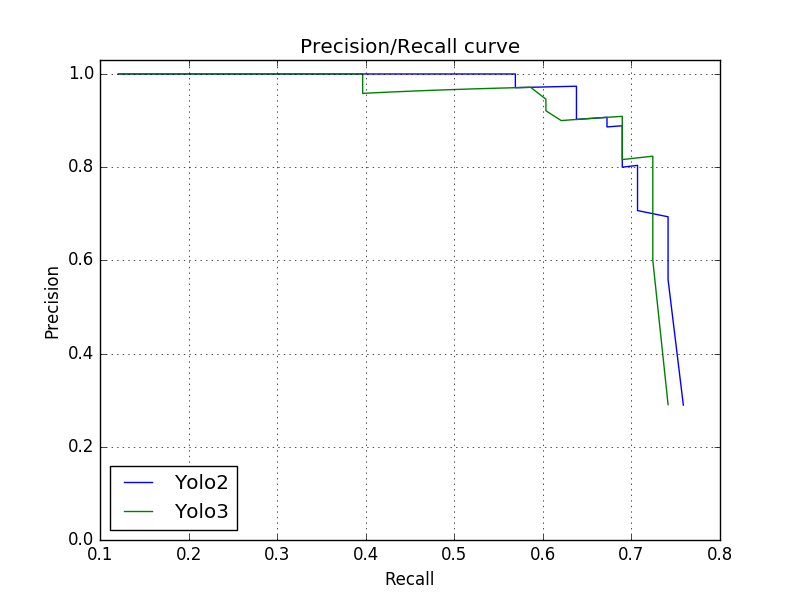
\includegraphics[width=0.8\linewidth]{results/case_buildings/prec_recall/yolo/bb.png}
  \caption{Yolo tested on bbnb}
  \label{fig:sfig1}
\end{subfigure}%
\begin{subfigure}{.5\textwidth}
  \centering
  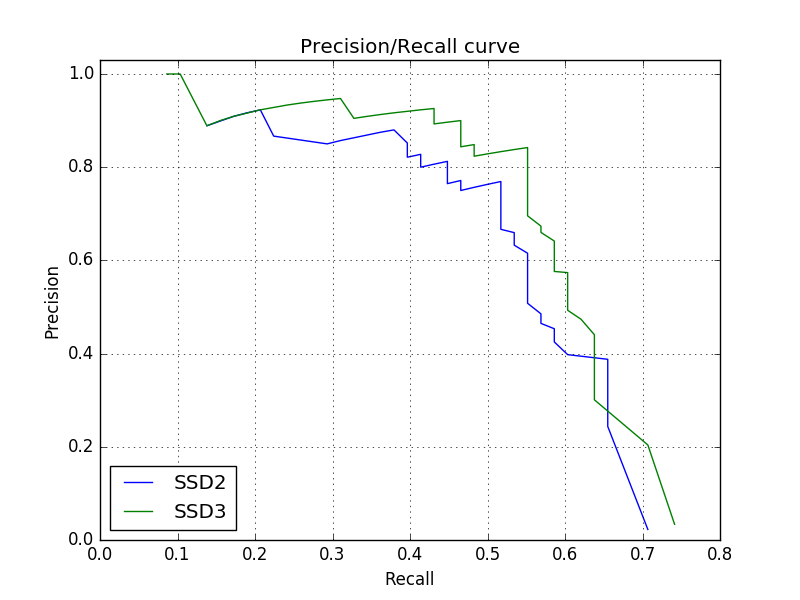
\includegraphics[width=.8\linewidth]{results/case_buildings/prec_recall/ssd/bb.png}
  \caption{SSD tested on bbnb}
  \label{fig:sfig2}
\end{subfigure}

\begin{subfigure}{.5\textwidth}
  \centering
  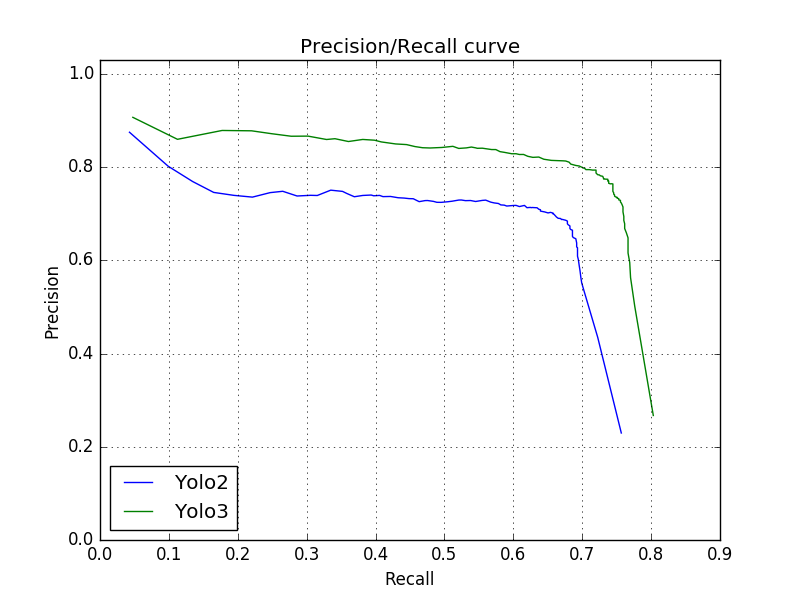
\includegraphics[width=0.8\linewidth]{results/case_buildings/prec_recall/yolo/bcbf.png}
  \caption{Yolo tested on bc, bf}
  \label{fig:sfig1}
\end{subfigure}%
\begin{subfigure}{.5\textwidth}
  \centering
  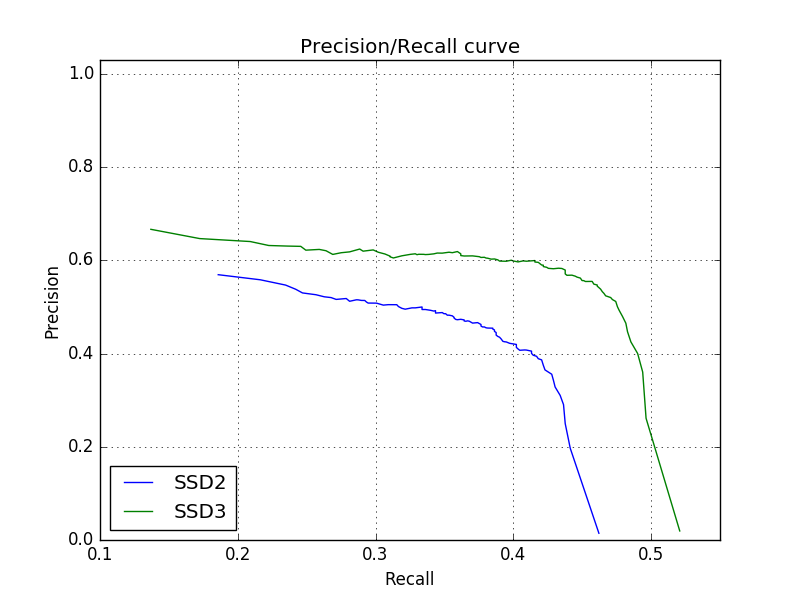
\includegraphics[width=.8\linewidth]{results/case_buildings/prec_recall/ssd/bcbf.png}
  \caption{SSD tested on bc, bf}
  \label{fig:sfig2}
\end{subfigure}

\begin{subfigure}{.5\textwidth}
  \centering
  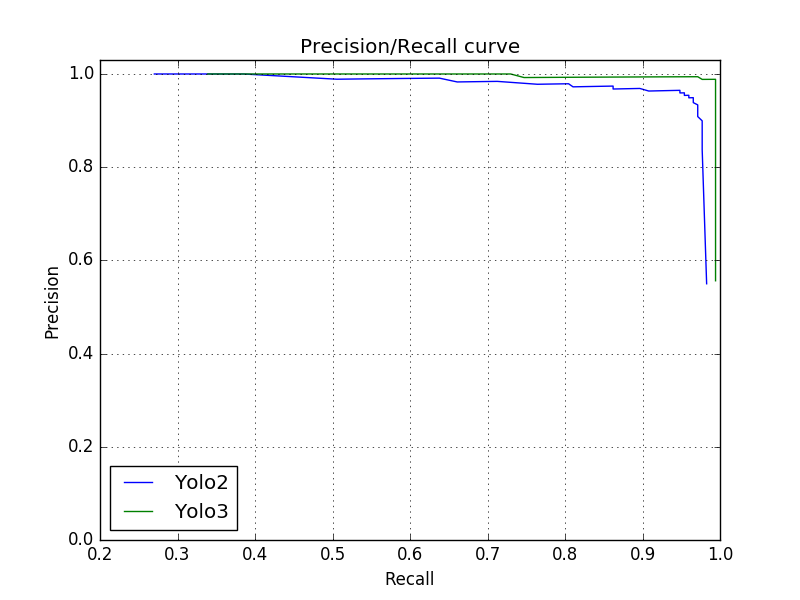
\includegraphics[width=0.8\linewidth]{results/case_buildings/prec_recall/yolo/trf.png}
  \caption{Yolo tested on trf}
  \label{fig:sfig1}
\end{subfigure}%
\begin{subfigure}{.5\textwidth}
  \centering
  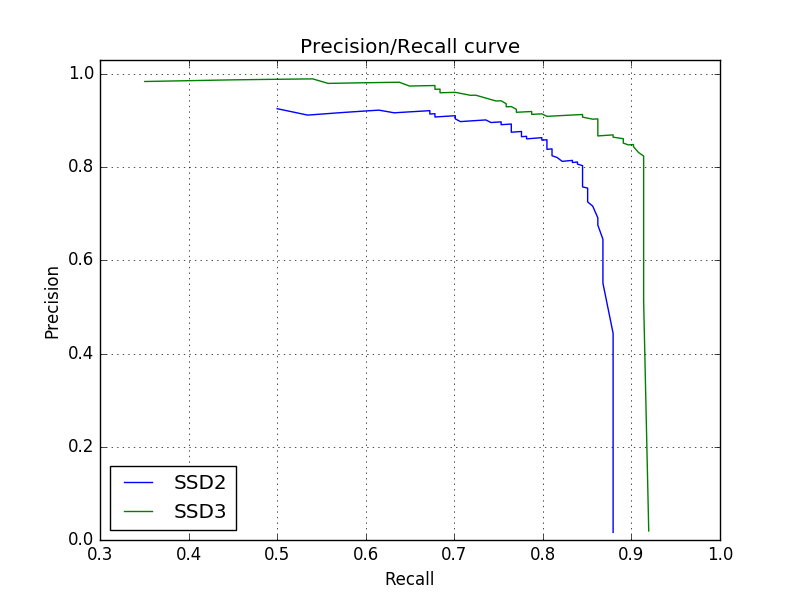
\includegraphics[width=.8\linewidth]{results/case_buildings/prec_recall/ssd/trf.png}
  \caption{SSD tested on trf}
  \label{fig:sfig2}
\end{subfigure}

\begin{subfigure}{.5\textwidth}
  \centering
  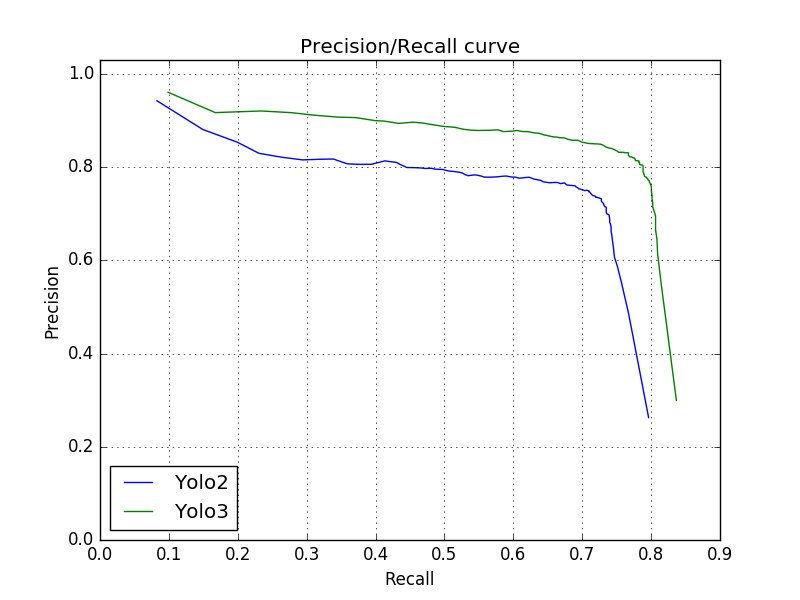
\includegraphics[width=0.8\linewidth]{results/case_buildings/prec_recall/yolo/bcbftrf.png}
  \caption{Yolo tested on bd, bf, trf}
  \label{fig:sfig1}
\end{subfigure}%
\begin{subfigure}{.5\textwidth}
  \centering
  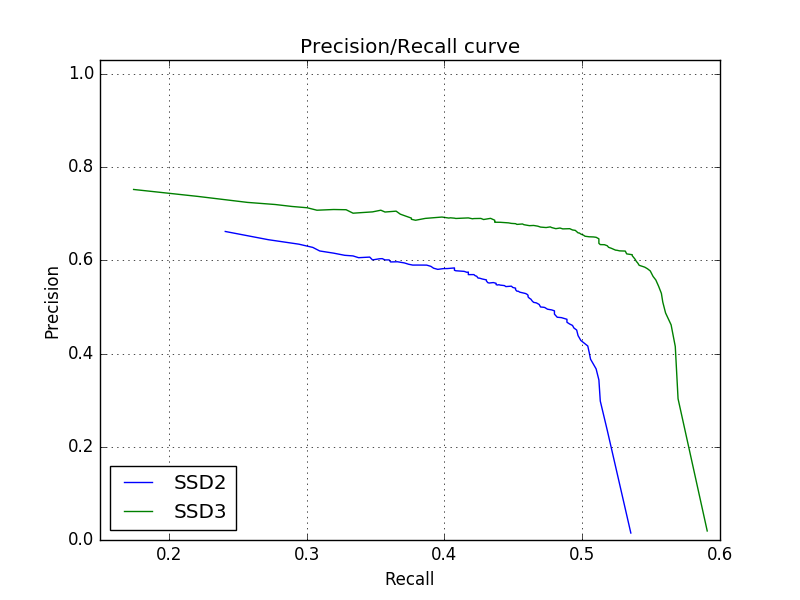
\includegraphics[width=.8\linewidth]{results/case_buildings/prec_recall/ssd/bcbftrf.png}
  \caption{SSD tested on bc, bf, trf}
  \label{fig:sfig2}
\end{subfigure}
\caption{Precision/recall curves of Yolo2, Yolo3, SSD2 and SSD3}
\label{fig:case_build}
\end{figure}

\newpage


\subsection{Tested on bbnb}

The hypothesis before running the experiment was that the bbnb dataset would be the most positively affected by training on a building class. Since \textit{bbnb} consists of mostly moored boats, where there are images that contain buildings close to sea level one could suspect could be mistaken as boats, as shown in \ref{img:bbnb_ex}. The building in the bottom left corner is close to sea level, while also being relatively close in size to the boats compared to the other buildings in the image, which makes it a good candidate for a misclassification. However, neither Yolo2 nor SSD2 classifies this building as a boat. All the detectors, Yolo2, Yolo3, SSD2 and SSD3 detects all the boats in the image. Both SSD2 and SSD3 detects the rightmost boat two times, and the bounding box differences between Yolo2 and Yolo3 and between SSD2 and SSD3 are so insignificant that training on the building class does not seem to help improve performance on this particular image. Both Yolo3 and ssd3 detects the buildings in the image well, as can be seen in figure \ref{fig:ex_bbnb_yolo3} and \ref{fig:ex_bbnb_ssd3}.


\begin{figure}[h!]
\begin{subfigure}{.5\textwidth}
  \centering
  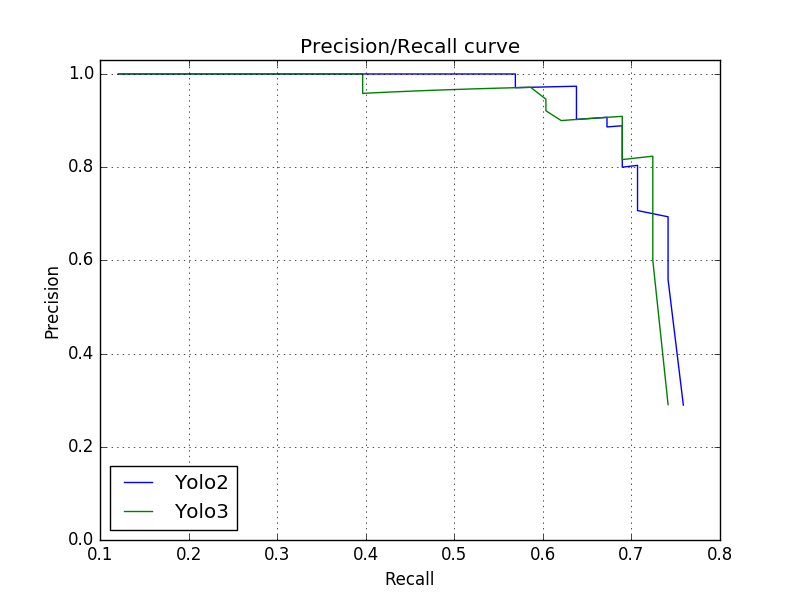
\includegraphics[width=0.8\linewidth]{results/case_buildings/prec_recall/yolo/bb.png}
  \caption{Yolo tested on bbnb}
  \label{fig:ex_bnbb_prec_rec_yolo}
\end{subfigure}%
\begin{subfigure}{.5\textwidth}
  \centering
  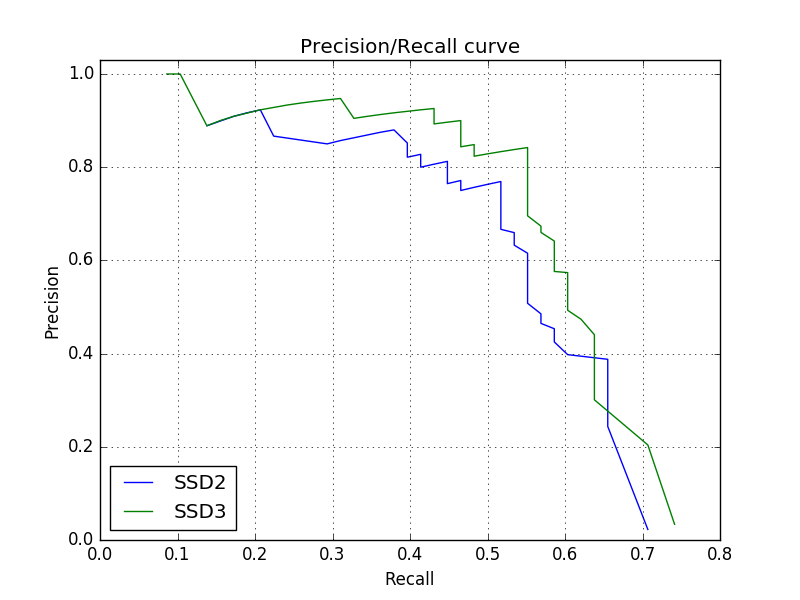
\includegraphics[width=.8\linewidth]{results/case_buildings/prec_recall/ssd/bb.png}
  \caption{SSD tested on bbnb}
  \label{fig:ex_bnbb_prec_rec_ssd}
\end{subfigure}
\begin{subfigure}{.5\textwidth}
  \centering
  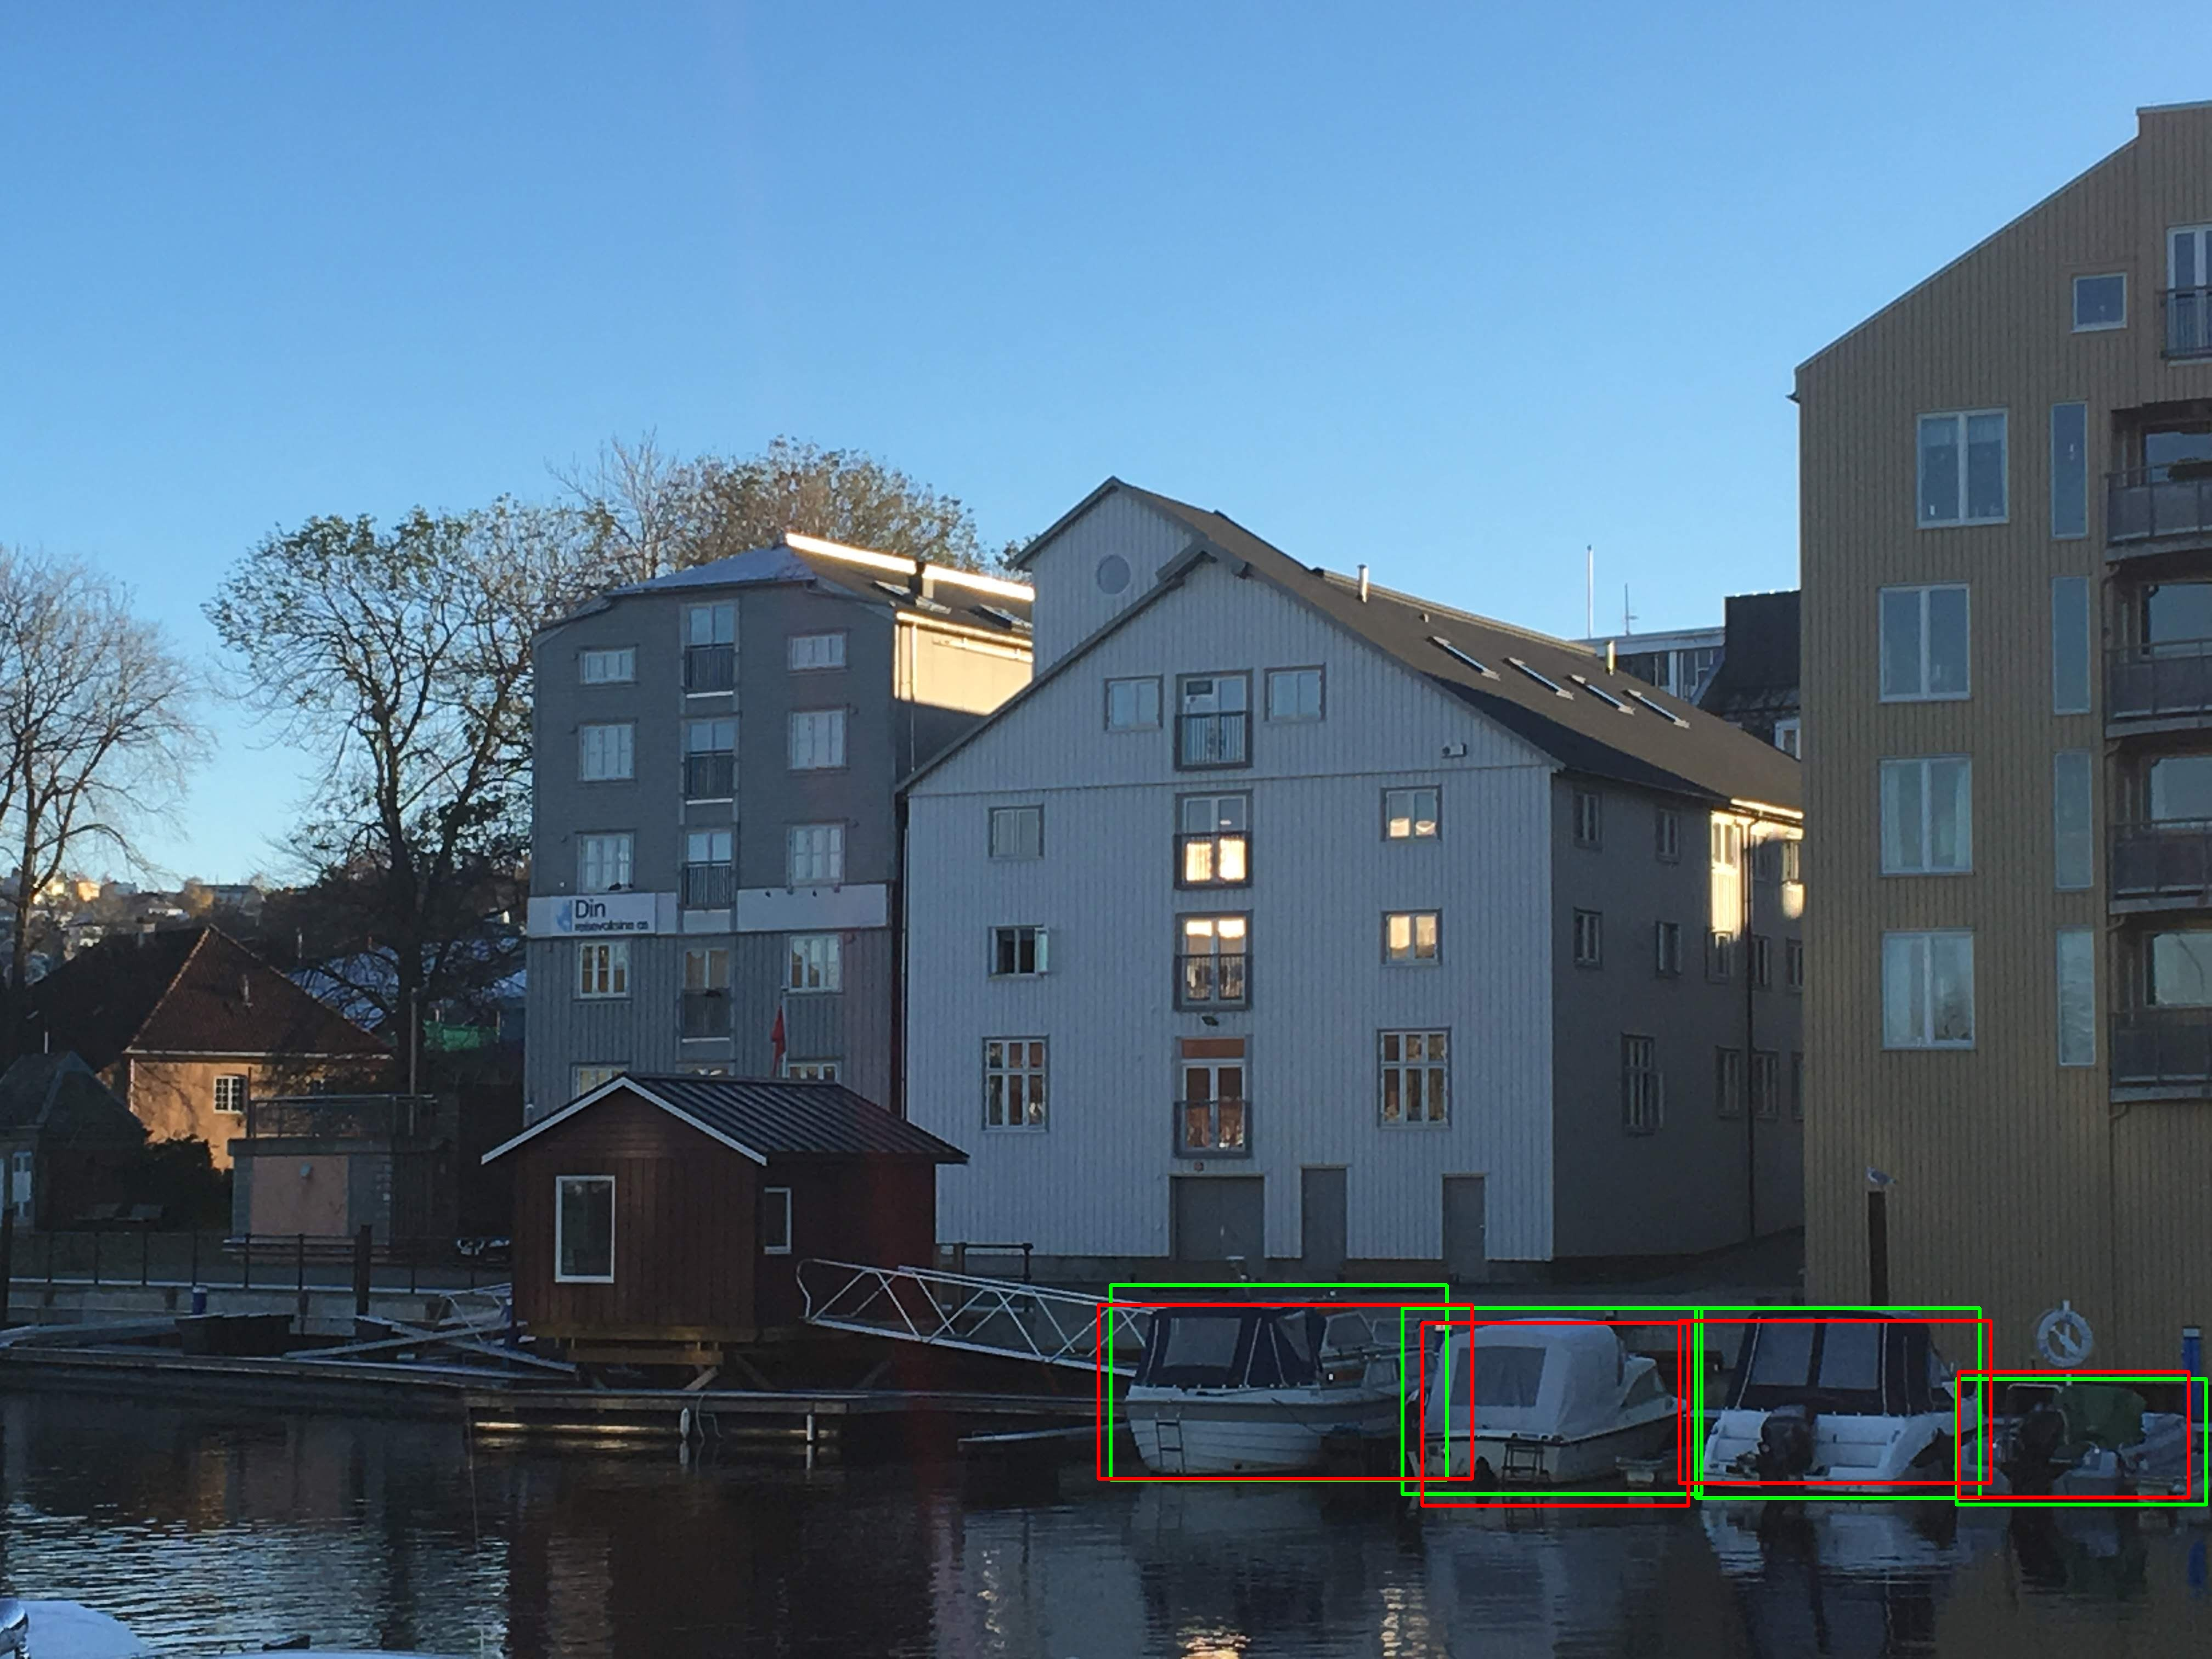
\includegraphics[width=0.8\linewidth]{results/case_buildings/prec_recall/yolo/IMG_2077_bbnb.jpg}
  \caption{Yolo2}
  \label{fig:ex_bbnb_yolo2}
\end{subfigure}%
\begin{subfigure}{.5\textwidth}
  \centering
  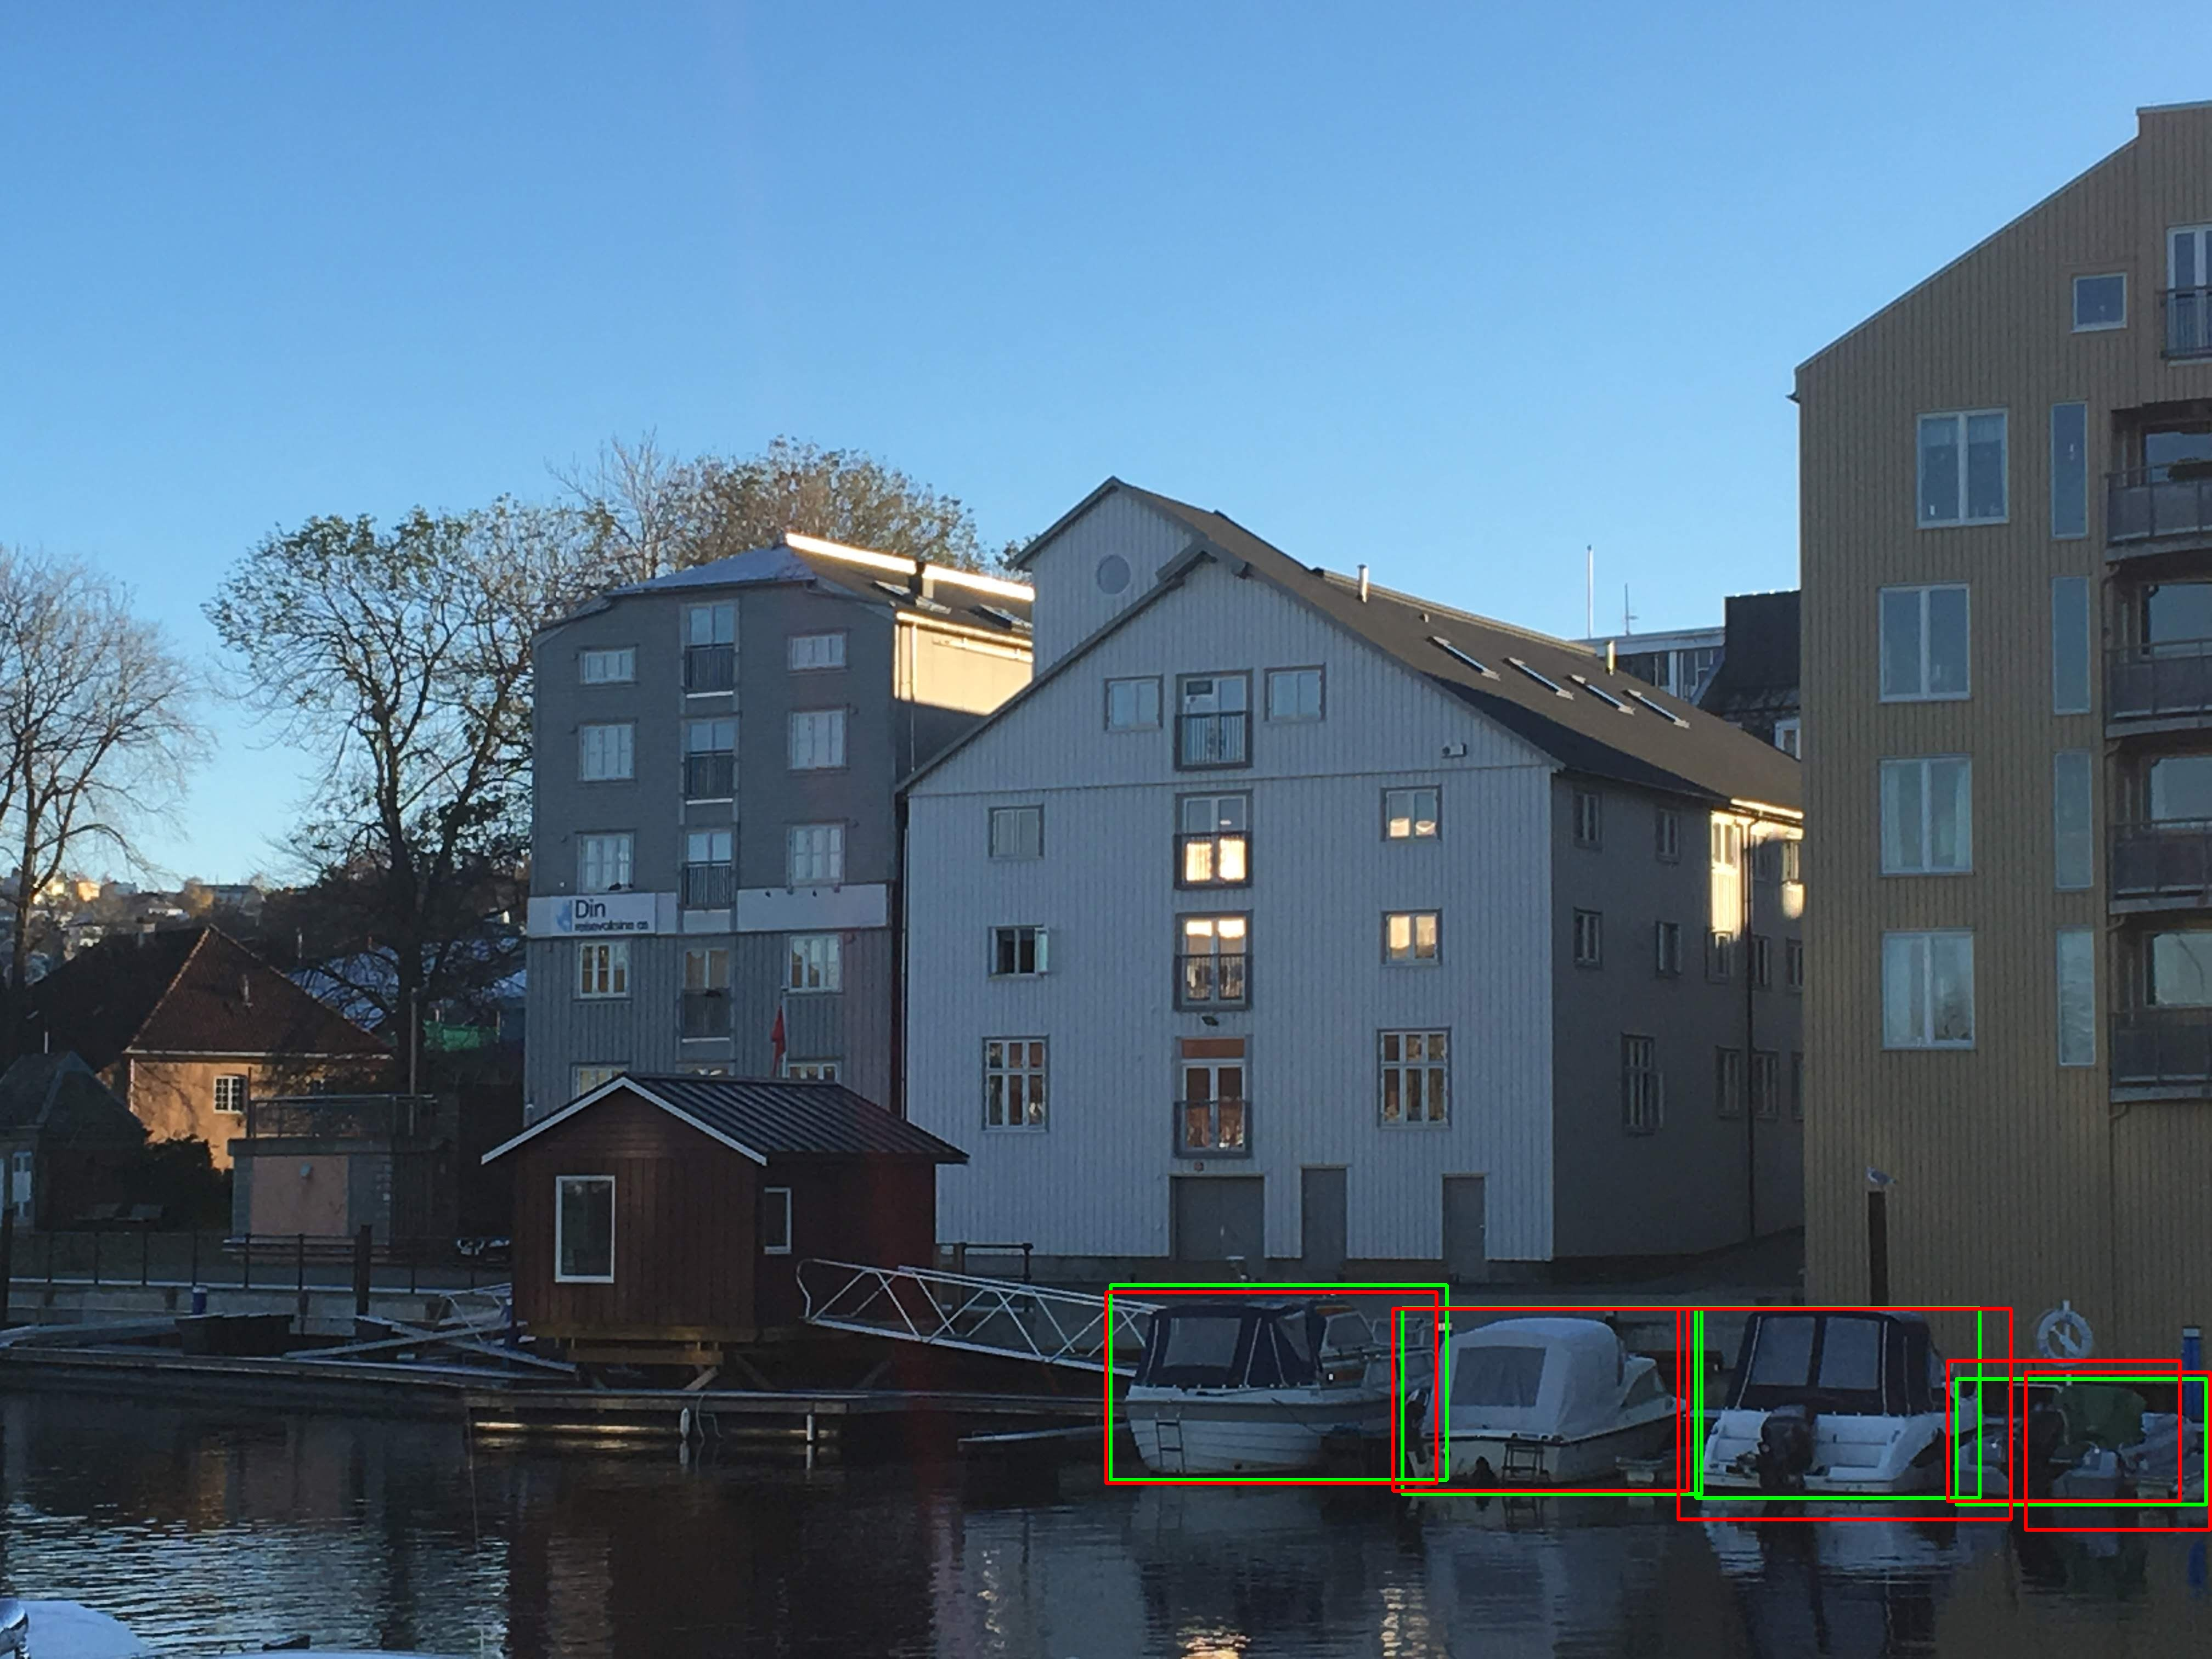
\includegraphics[width=.8\linewidth]{results/case_buildings/prec_recall/ssd/IMG_2077_bbnb.jpg}
  \caption{SSD2}
  \label{fig:ex_bbnb_ssd2}
\end{subfigure}

\begin{subfigure}{.5\textwidth}
  \centering
  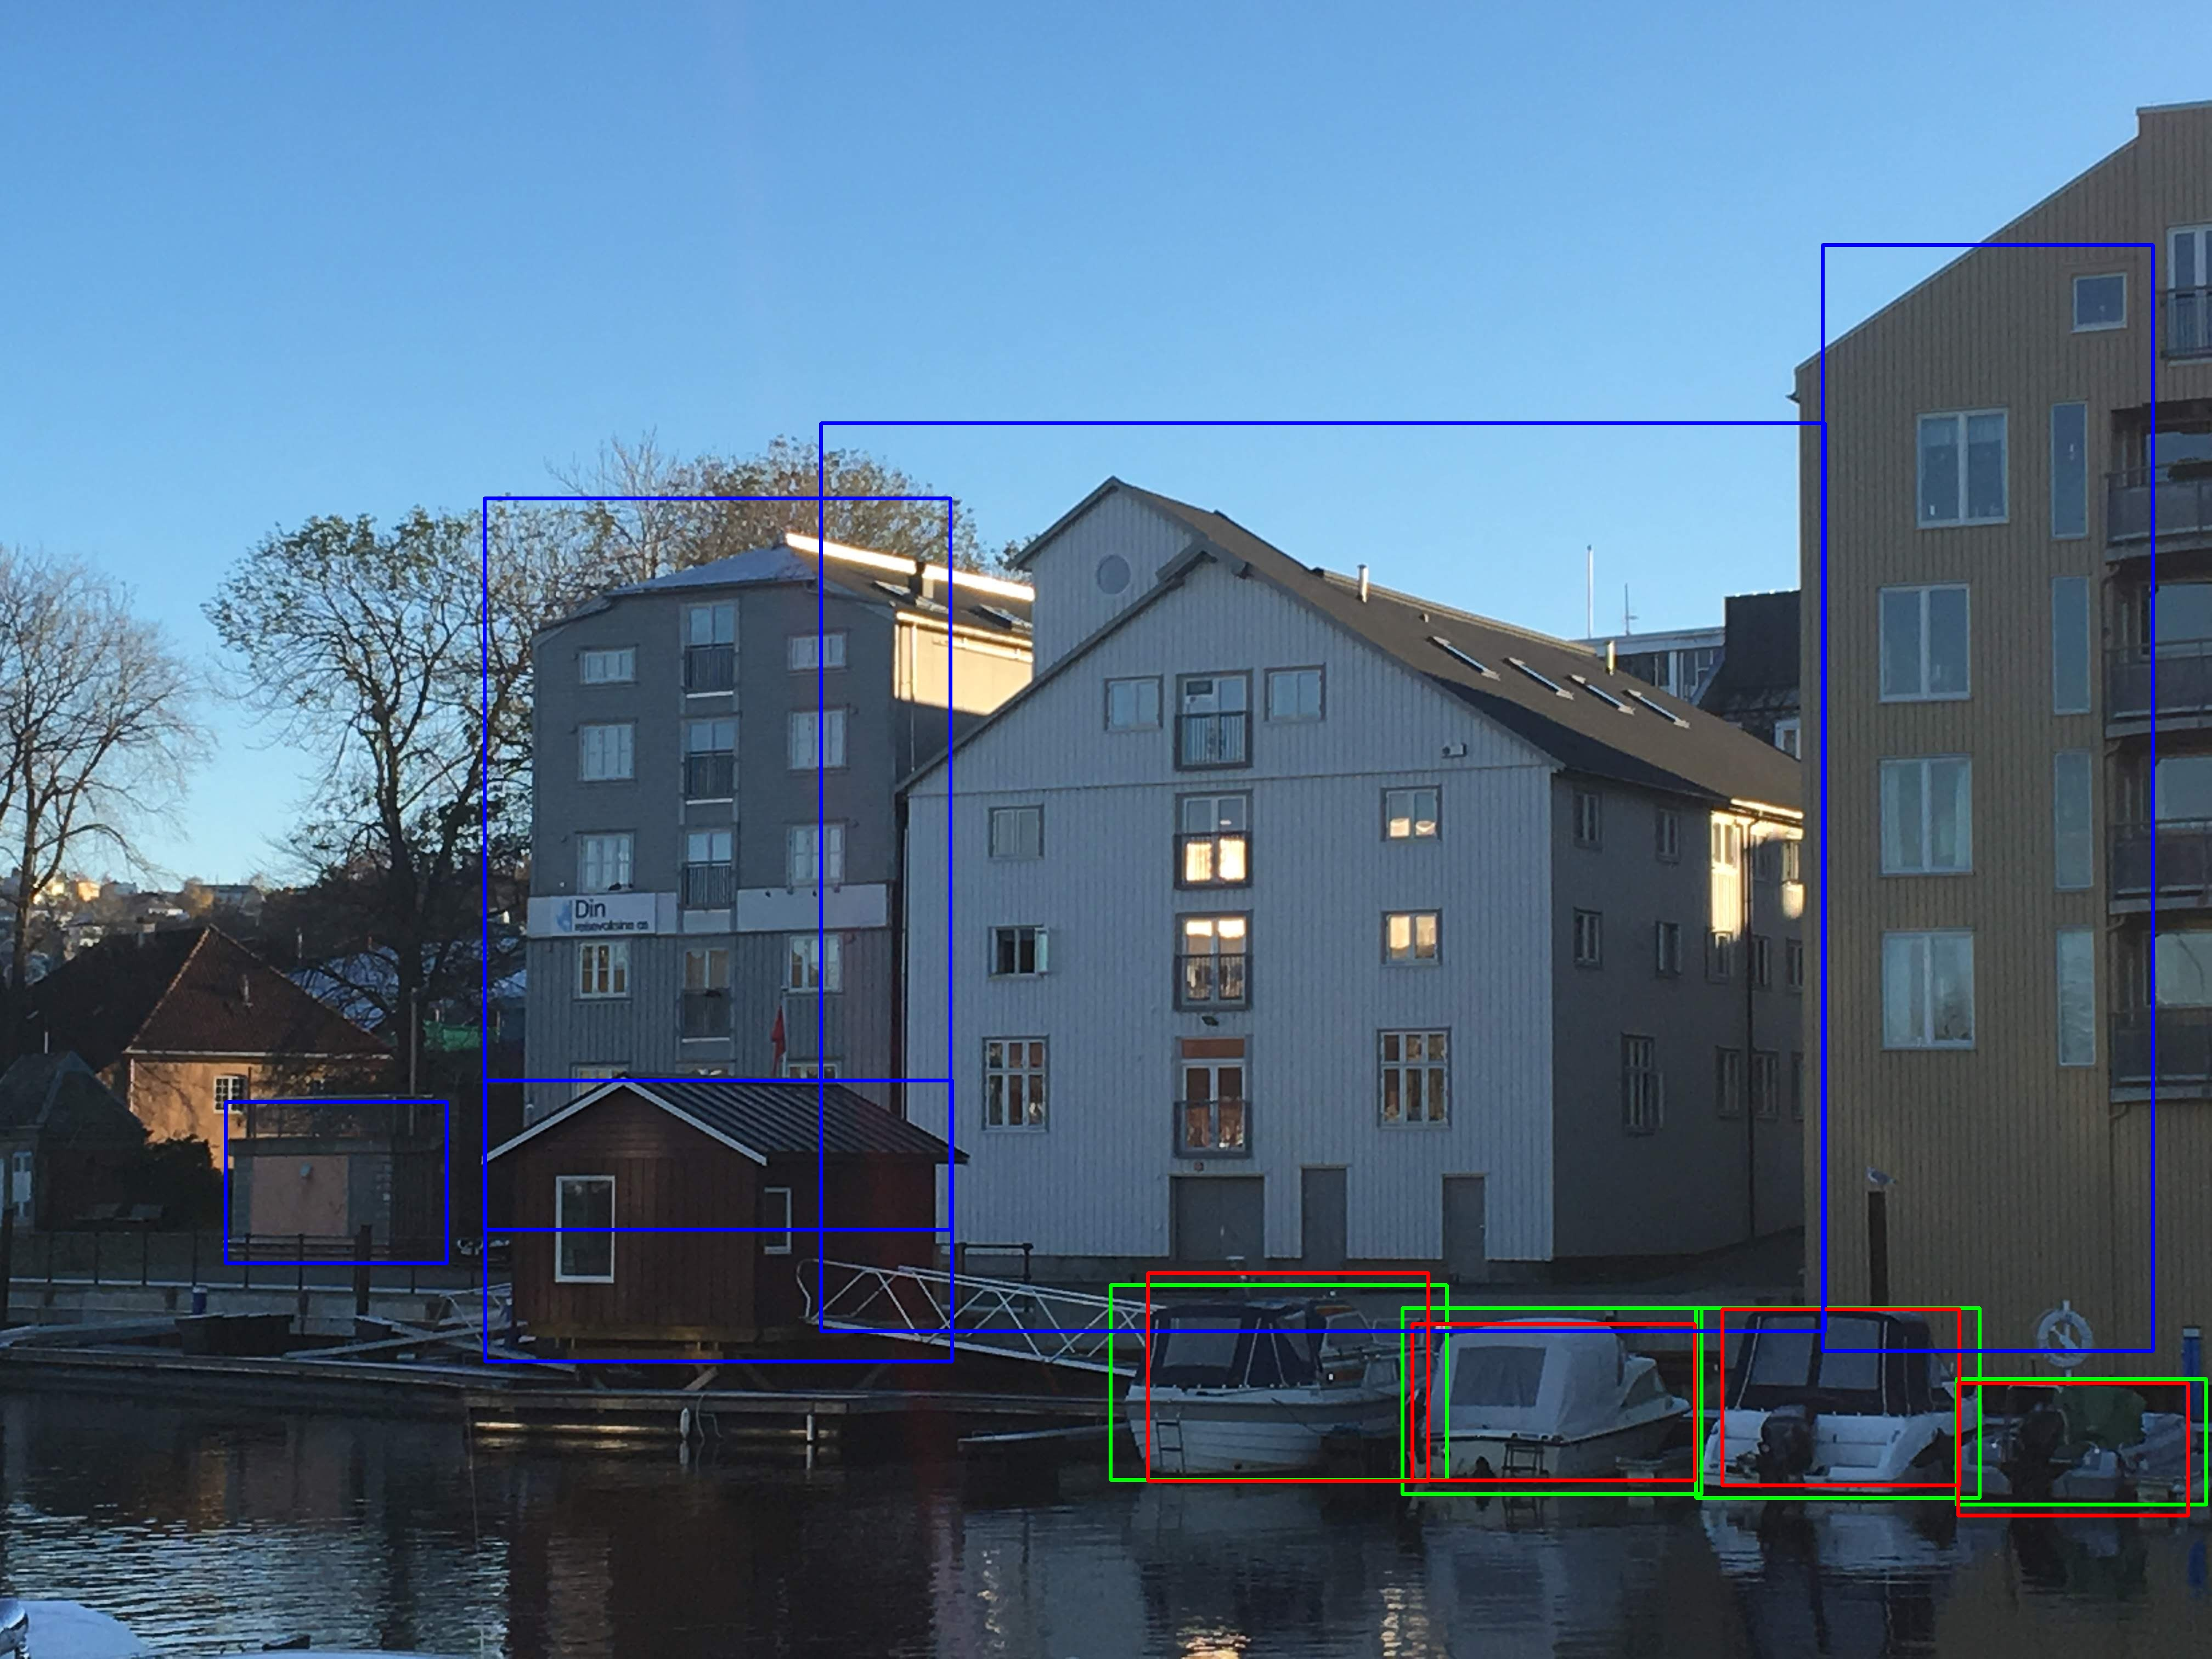
\includegraphics[width=0.8\linewidth]{results/case_buildings/prec_recall/yolo/IMG_2077_build.jpg}
  \caption{Yolo3}
  \label{fig:ex_bbnb_yolo3}
\end{subfigure}%
\begin{subfigure}{.5\textwidth}
  \centering
  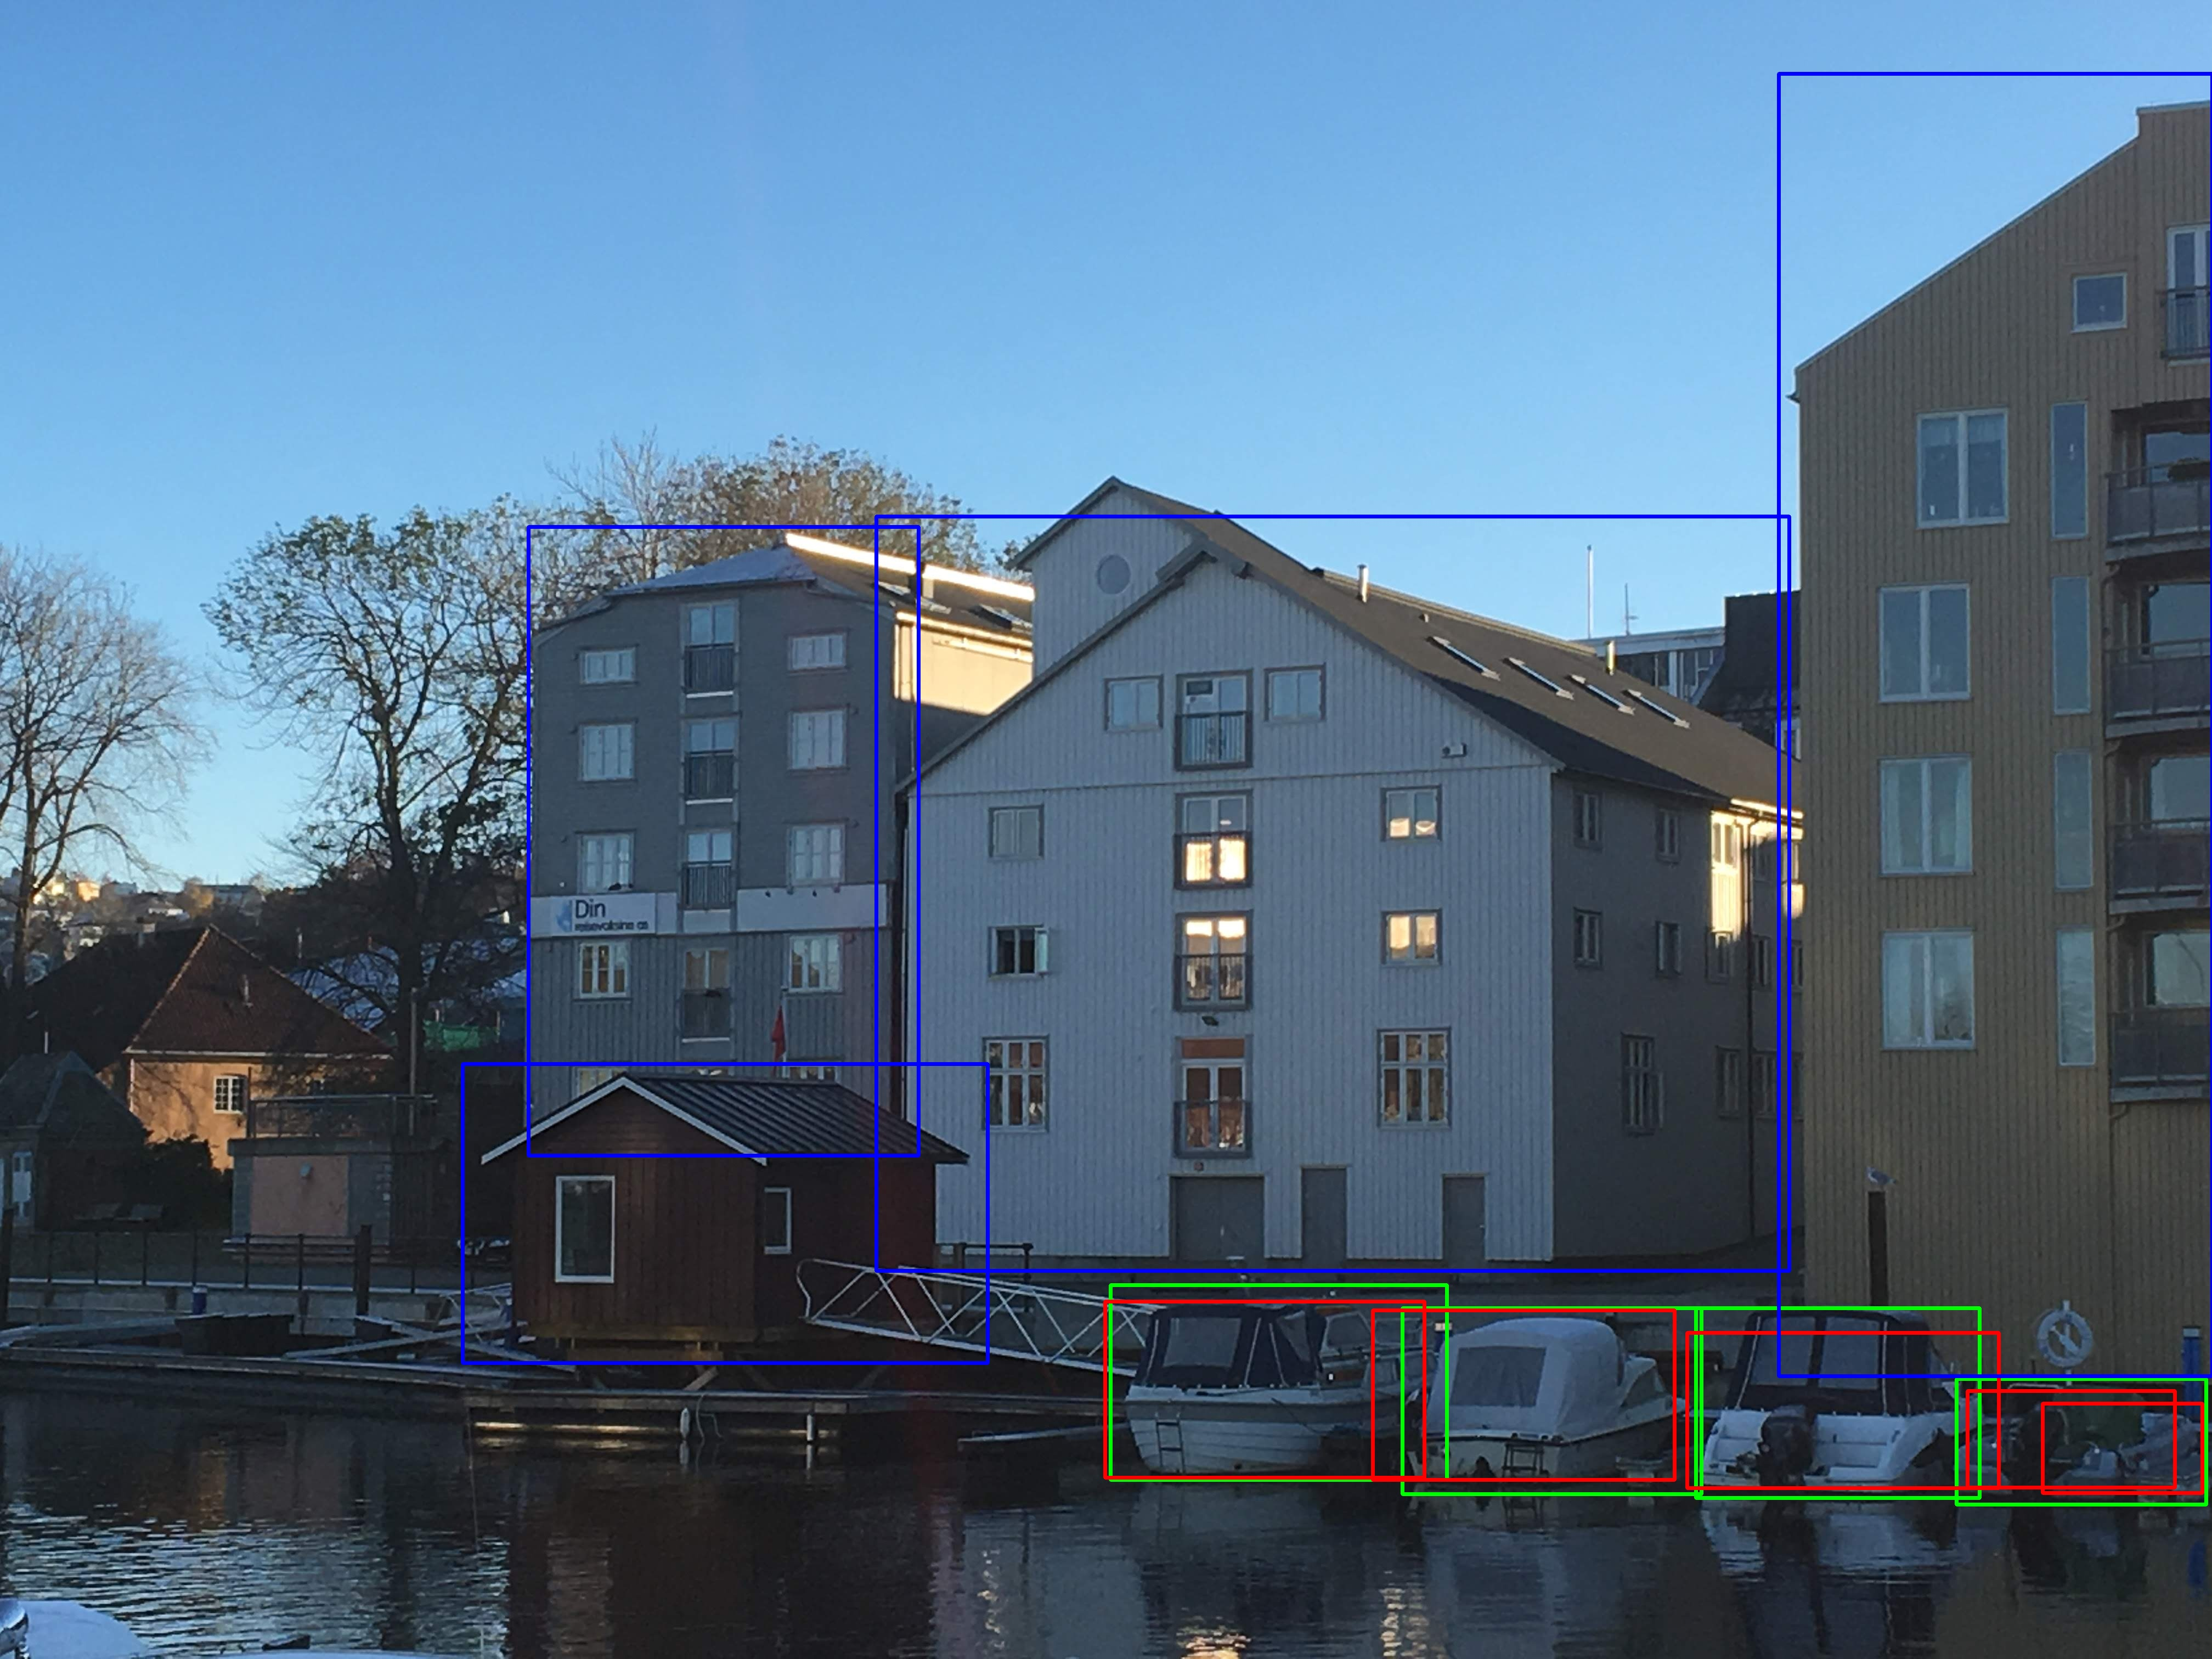
\includegraphics[width=.8\linewidth]{results/case_buildings/prec_recall/ssd/IMG_2077_build.jpg}
  \caption{SSD3}
  \label{fig:ex_bbnb_ssd3}
\end{subfigure}
\caption{Yolo2, Yolo3, SSD2, SSD3 example image from \textit{bbnb} test set. Green bounding boxes are ground truth, red bounding boxes are detected boats, blue bounding boxes are detected buildings}
\label{img:bbnb_ex}
\end{figure}

\newpage

\subsection{Tested on bc, bf}

The datasets \textit{bc} and \textit{bf} consists mostly of images taken towards open sea, of boats that are sailing, i.e., the boats are not moored. It is on this dataset the performance differences between Yolo2 and Yolo3 and between SSD2 and SSD3 differ the most, as can be seen in figure \ref{fig:bcbf_prec}.

\begin{figure}[h!]
\begin{subfigure}{.5\textwidth}
  \centering
  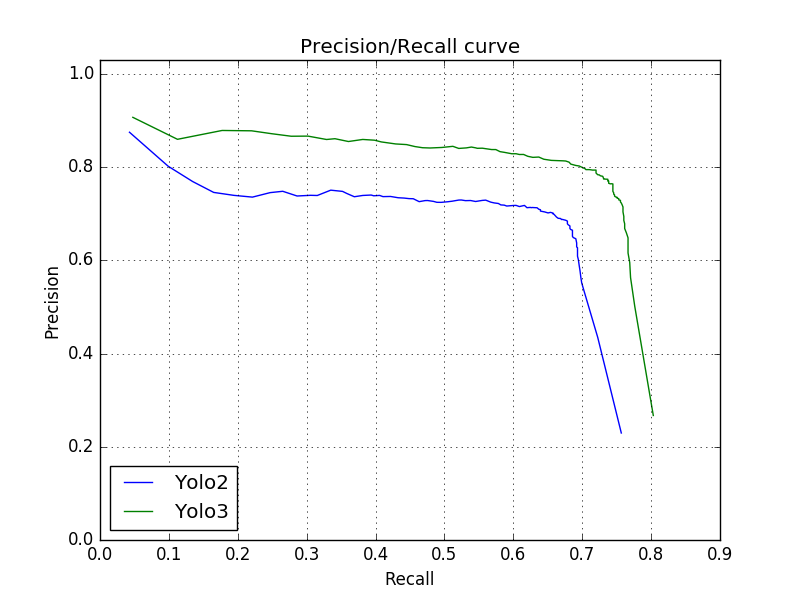
\includegraphics[width=0.8\linewidth]{results/case_buildings/prec_recall/yolo/bcbf.png}
  \caption{Yolo tested on bc, bf}
  \label{fig:ex_bcbf_prec_rec_yolo}
\end{subfigure}%
\begin{subfigure}{.5\textwidth}
  \centering
  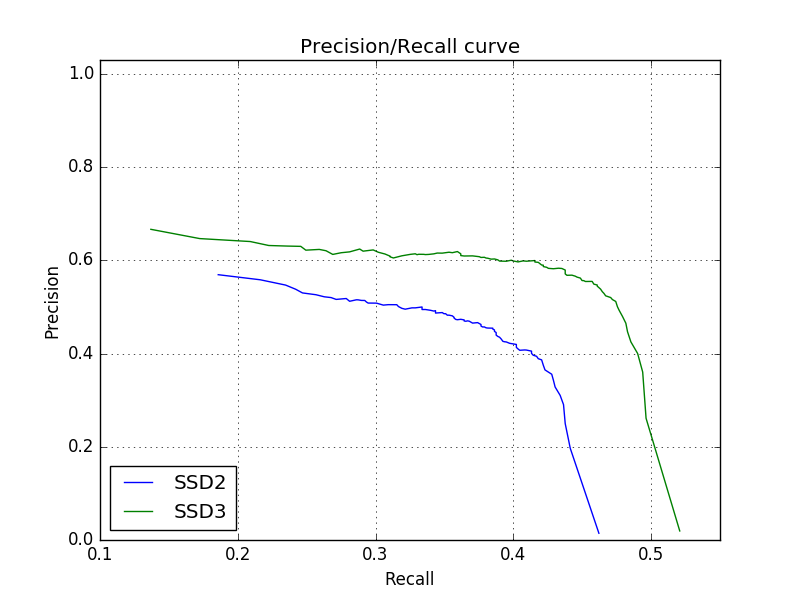
\includegraphics[width=.8\linewidth]{results/case_buildings/prec_recall/ssd/bcbf.png}
  \caption{SSD tested on bc, bf}
  \label{fig:ex_bcbf_prec_rec_ssd}
\end{subfigure}
\caption{Yolo2, Yolo3, SSD2, SSD3 example image from \textit{bbnb} test set. Green bounding boxes are ground truth, red bounding boxes are detected boats, blue bounding boxes are detected buildings}
\label{fig:bcbf_prec}
\end{figure}

\vspace{3mm}

By going through the around 300 test images, some differences between the models become apparent. While the differences between SSD2 and SSD3 are somewhat obvious, the difference between Yolo2 and Yolo3 are more nuanced. 

\subsubsection{SSD2 and SSD3 on bc, bf}
In around 10 percent of the test images, SSD2 detects land as a boat, in none of these images does SSD3 perform the same way. An example of this is shown in figure \ref{img:bixbox_ssd}. More examples of this behavior can be found in Appendix C in chapter \ref{sec:bigbox}

\begin{figure}[h!]
\begin{subfigure}{.5\textwidth}
  \centering
  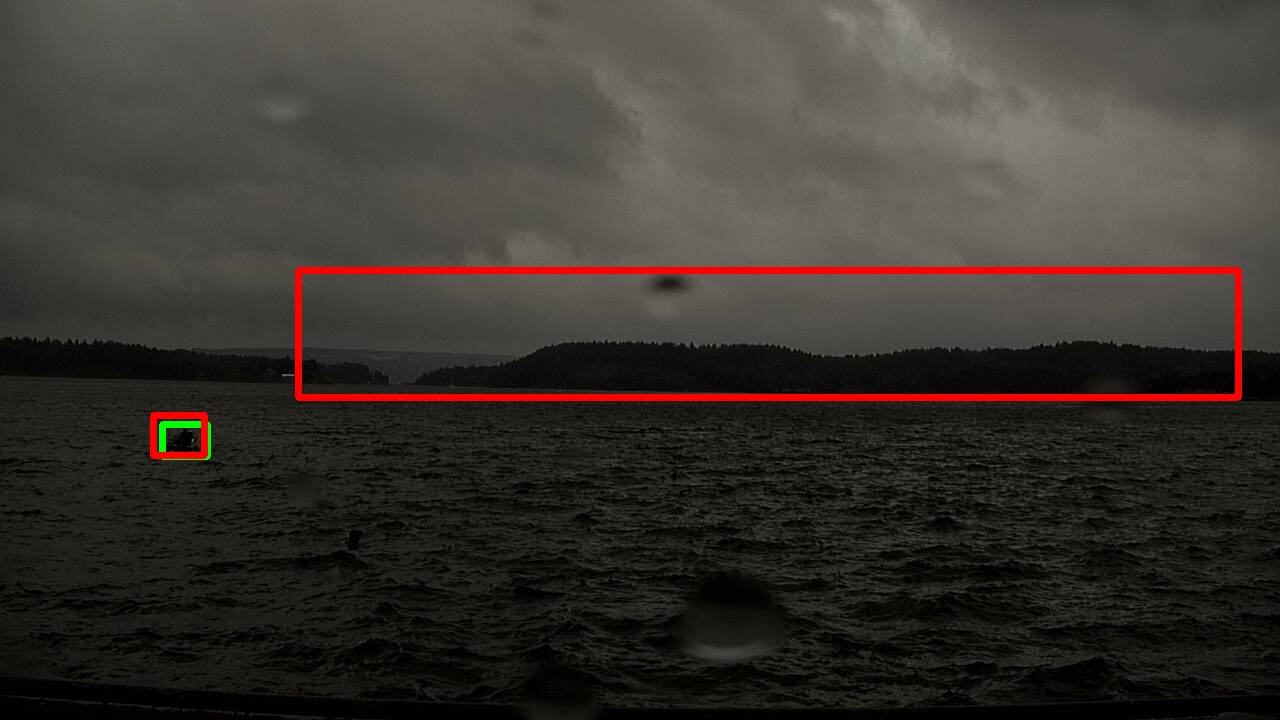
\includegraphics[width=0.9\linewidth]{results/case_buildings/bigbox_bcbf/SSD2/selected_06_14_axis0049.jpg}
  \caption{SSD2}
  \label{fig:big_box_ssd2}
\end{subfigure}%
\begin{subfigure}{.5\textwidth}
  \centering
  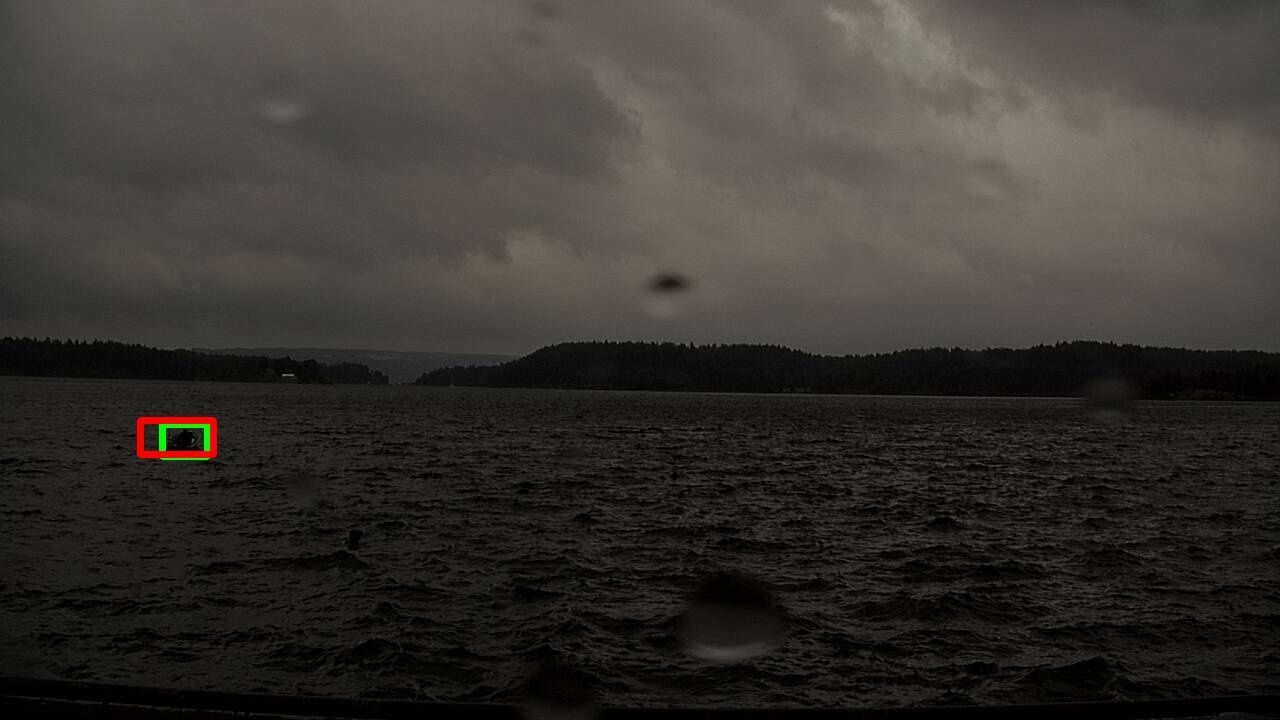
\includegraphics[width=.9\linewidth]{results/case_buildings/bigbox_bcbf/SSD3/selected_06_14_axis0049.jpg}
  \caption{SSD3}
  \label{fig:big_box_ssd3}
\end{subfigure}
\caption{SSD2 detects land as boat. Red bounding boxes are boat detections, green bounding boxes are ground truth.}
\label{img:bixbox_ssd}
\end{figure}

There are also some examples where SSD2 misclassifies buildings as boats, while SSD3 does not. One example is shown in figure \ref{img:misclass_ssd}

\begin{figure}[h!]
\begin{subfigure}{.5\textwidth}
  \centering
  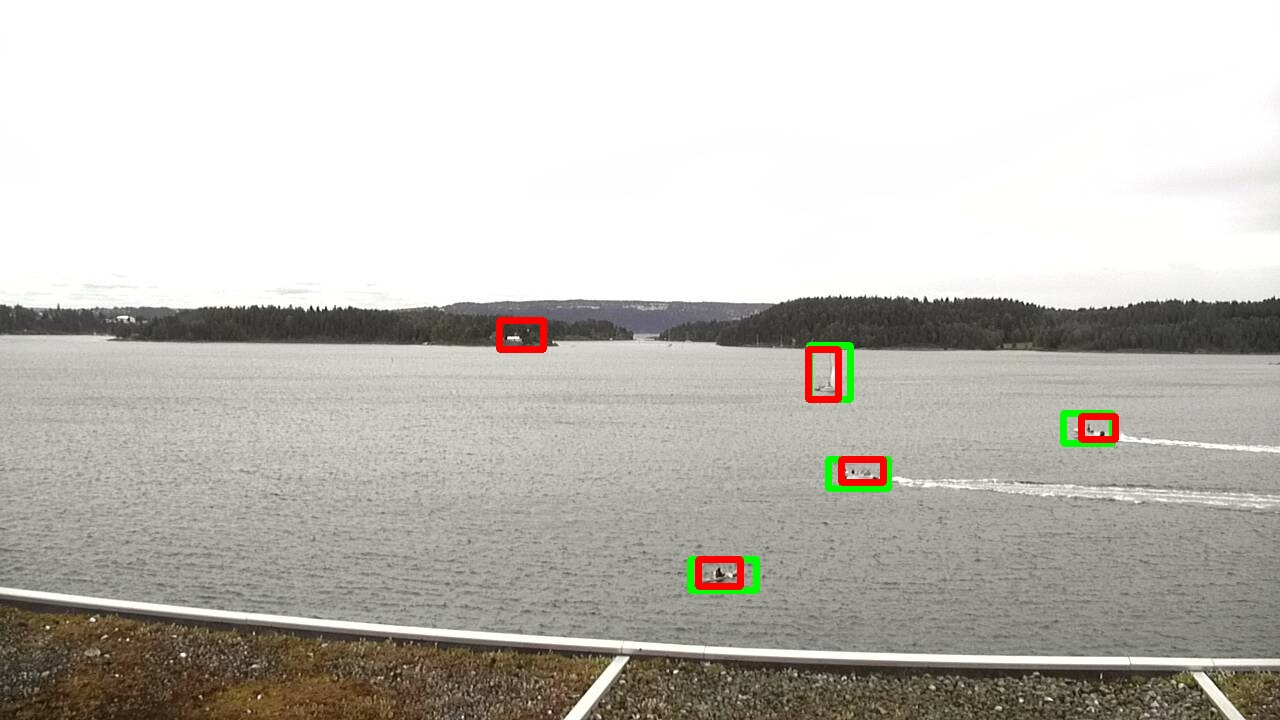
\includegraphics[width=0.9\linewidth]{results/case_buildings/misclass/selected_08_07_frame11982_bbnb.jpg}
  \caption{SSD2}
  \label{fig:misclass_ssd2}
\end{subfigure}%
\begin{subfigure}{.5\textwidth}
  \centering
  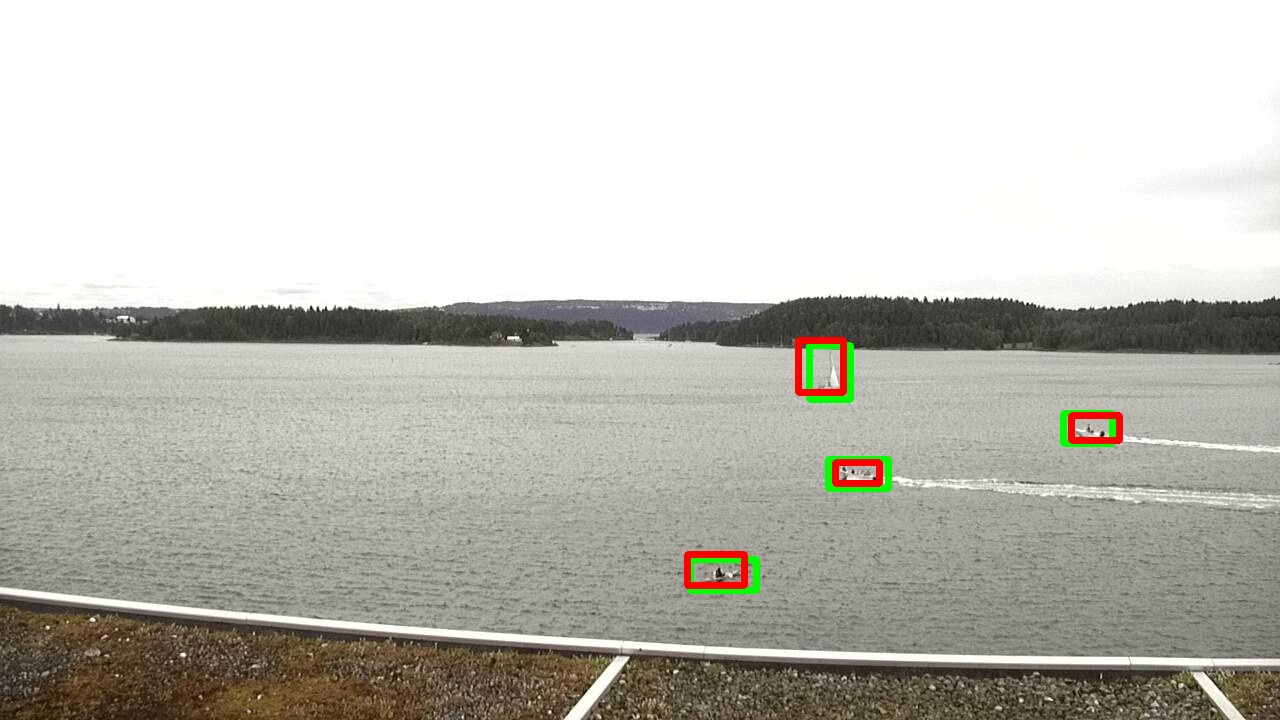
\includegraphics[width=.9\linewidth]{results/case_buildings/misclass/selected_08_07_frame11982_build.jpg}
  \caption{SSD3}
  \label{fig:misclass_ssd3}
\end{subfigure}
\caption{Leftmost red bounding box in SSD2 is a detection of a building as a boat, this is not detected as a boat in SSD3. Red bounding boxes are boat detections, green bounding boxes are ground truth.}
\label{img:misclass_ssd}
\end{figure}

\vspace{3mm}
\newpage

\subsubsection{Yolo2 and Yolo3 on bc, bf}

As mentioned Yolo2 and Yolo3 does not differ as clearly as SSD2 and SSD3. There are examples of Yolo2 performing better than Yolo3 and vice versa. In many of the misclassifications in the test data both Yolo2 and Yolo3 mistakes the same object as a boat. By analyzing the results from both Yolo2 and Yolo3, the following tendencies can be seen:

\begin{itemize}
    \item Yolo2 and Yolo3 have the disposition to mistake the same objects as boats. See Appendix C chapter \ref{sec:same_mistake} for example images.
    \item Yolo2 performs better in some cases, while Yolo3 performs better in other. It is not clear what makes one better than the other in each specific case. See Appendix C chapter \ref{sec:3better} and \ref{sec:2better} for example images
    \item Yolo2 makes some misclassifications that could imply that training on a building class makes Yolo3 more robust to the more incomprehensible misclassifications. See appendix C chapter \ref{sec:yolo2_spec_misc} for example images.
\end{itemize}

As opposed to the differences between SSD2 and SSD3 the differences in the results between Yolo2 and Yolo3 are hard to pinpoint. Both Yolo2 and Yolo3 makes misclassifications, but Yolo2 seems to make slightly more than Yolo3. Yolo3 also avoids making some misclassifications Yolo2 makes in the background, as shown in figure \ref{img:misclass_yolo}.

\begin{figure}[h!]
\begin{subfigure}{.5\textwidth}
  \centering
  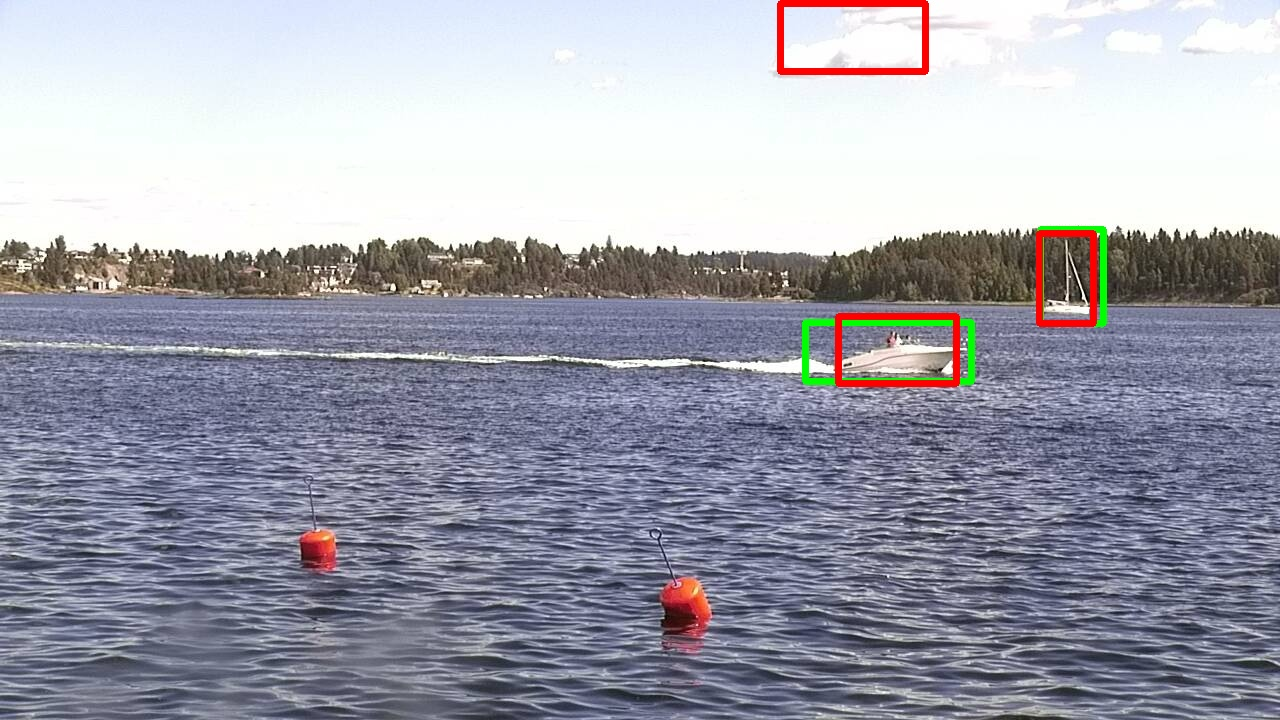
\includegraphics[width=0.9\linewidth]{results/case_buildings/yolo23/grove/yolo2/selected_06_25_frame0357.jpg}
  \caption{Yolo2}
  \label{fig:misclass_yolo2}
\end{subfigure}%
\begin{subfigure}{.5\textwidth}
  \centering
  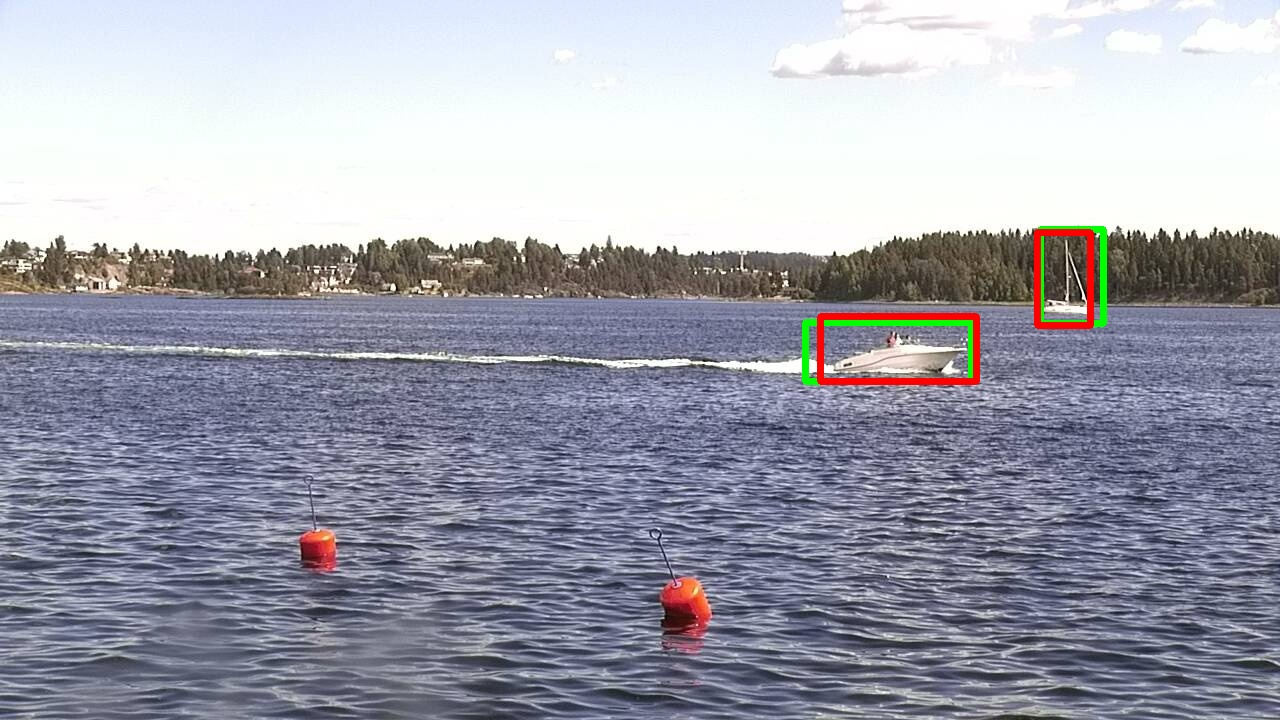
\includegraphics[width=.9\linewidth]{results/case_buildings/yolo23/grove/yolo3/selected_06_25_frame0357.jpg}
  \caption{Yolo3}
  \label{fig:misclass_yolo3}
\end{subfigure}
\caption{Yolo 2 misclassifies a cloud as a boat, Yolo3 does not. Red bounding boxes are detections, green bounding boxes are ground truth.}
\label{img:misclass_yolo}
\end{figure}

\newpage

\subsection{Tested on trf}

The precision/recall curve for Yolo2, Yolo3, SSD2, and SSD3 on trf can be seen in figure \ref{fig:trf_prec}. All the models perform very well on this dataset, where Yolo3 almost gets a perfect score with an average precision of 0.908, meaning it is very close to detect all the objects while having practically no misclassifications. This result could be an indication of overtraining on this dataset and will be discussed further in chapter \ref{dataset_divers}. 

\vspace{3mm}

Both the models trained on the building class, perform better than the model only trained on the boat class. As for the tests on bc and bf the differences between SSD2 and SSD3 are more evident than the differences between Yolo2 and Yolo3. The performance difference between SSD2 and SSD3 is also more significant than between Yolo2 and Yolo3, as can be seen in figure \ref{fig:trf_prec}


\begin{figure}[h!]
\begin{subfigure}{.5\textwidth}
  \centering
  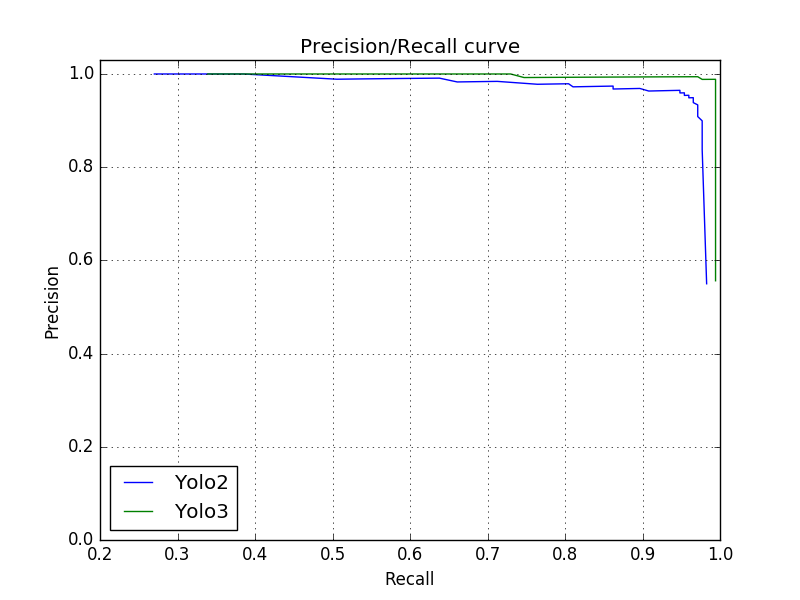
\includegraphics[width=0.8\linewidth]{results/case_buildings/prec_recall/yolo/trf.png}
  \caption{Yolo tested on trf}
  \label{fig:ex_trf_prec_rec_yolo}
\end{subfigure}%
\begin{subfigure}{.5\textwidth}
  \centering
  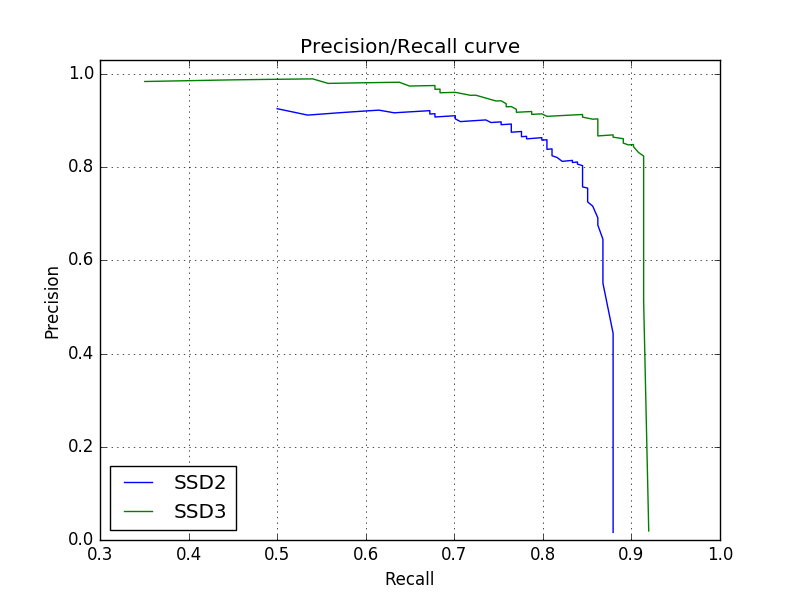
\includegraphics[width=.8\linewidth]{results/case_buildings/prec_recall/ssd/trf.png}
  \caption{SSD tested on trf}
  \label{fig:ex_trf_prec_rec_ssd}
\end{subfigure}
\caption{Precision/recall curves for Yolo2, Yolo3, SSD2 and SSD3 on trf}
\label{fig:trf_prec}
\end{figure}

\subsubsection{SSD2 and SSD3 on trf}

SSD2 has some of the same behaviors on trf as it had on bc and bf. For instance, it sometimes classifies land as a boat, as shown in figure \ref{fig:ssd_trf_bigbox}. More examples of this behavior can be seen in Appendix C, chapter \ref{fig:ssd_trf_bigbox}.

\begin{figure}[h!]
\begin{subfigure}{.5\textwidth}
  \centering
  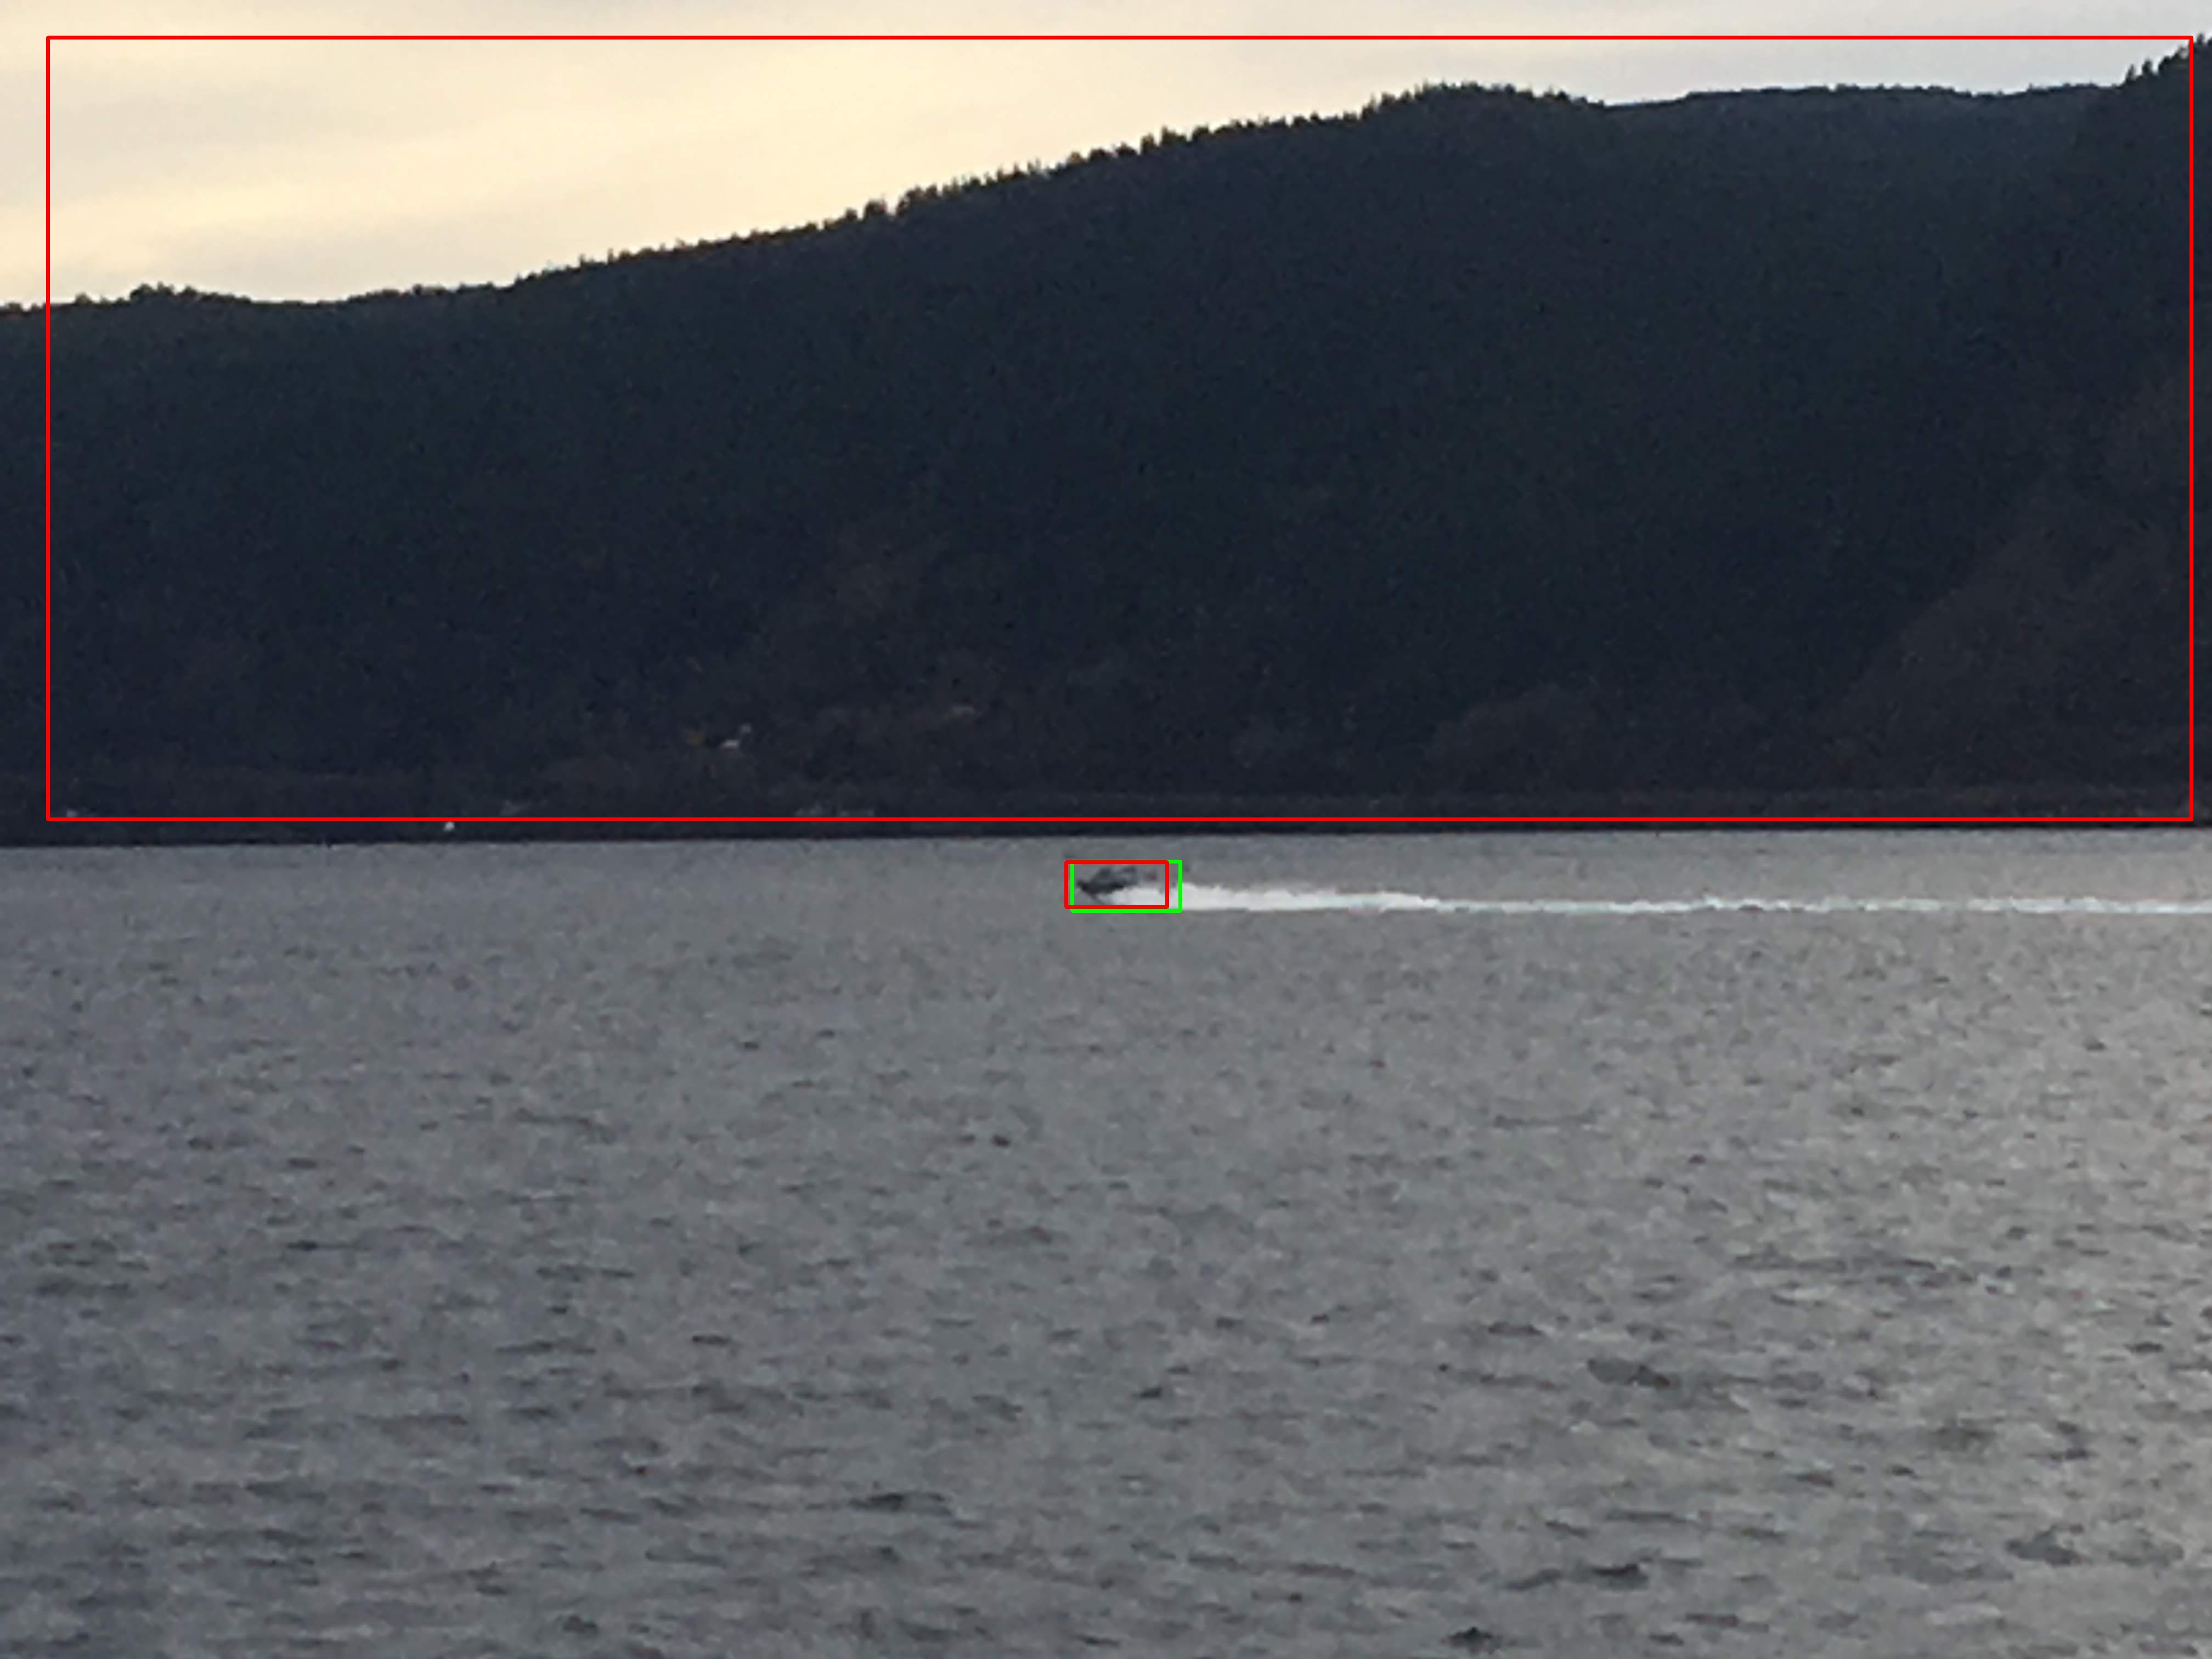
\includegraphics[width=0.8\linewidth]{results/case_buildings/ssdtrf/ssd2/grov2/IMG_2325.jpg}
  \caption{SSD2}
  \label{fig:ex_trf_prec_rec_yolo}
\end{subfigure}%
\begin{subfigure}{.5\textwidth}
  \centering
  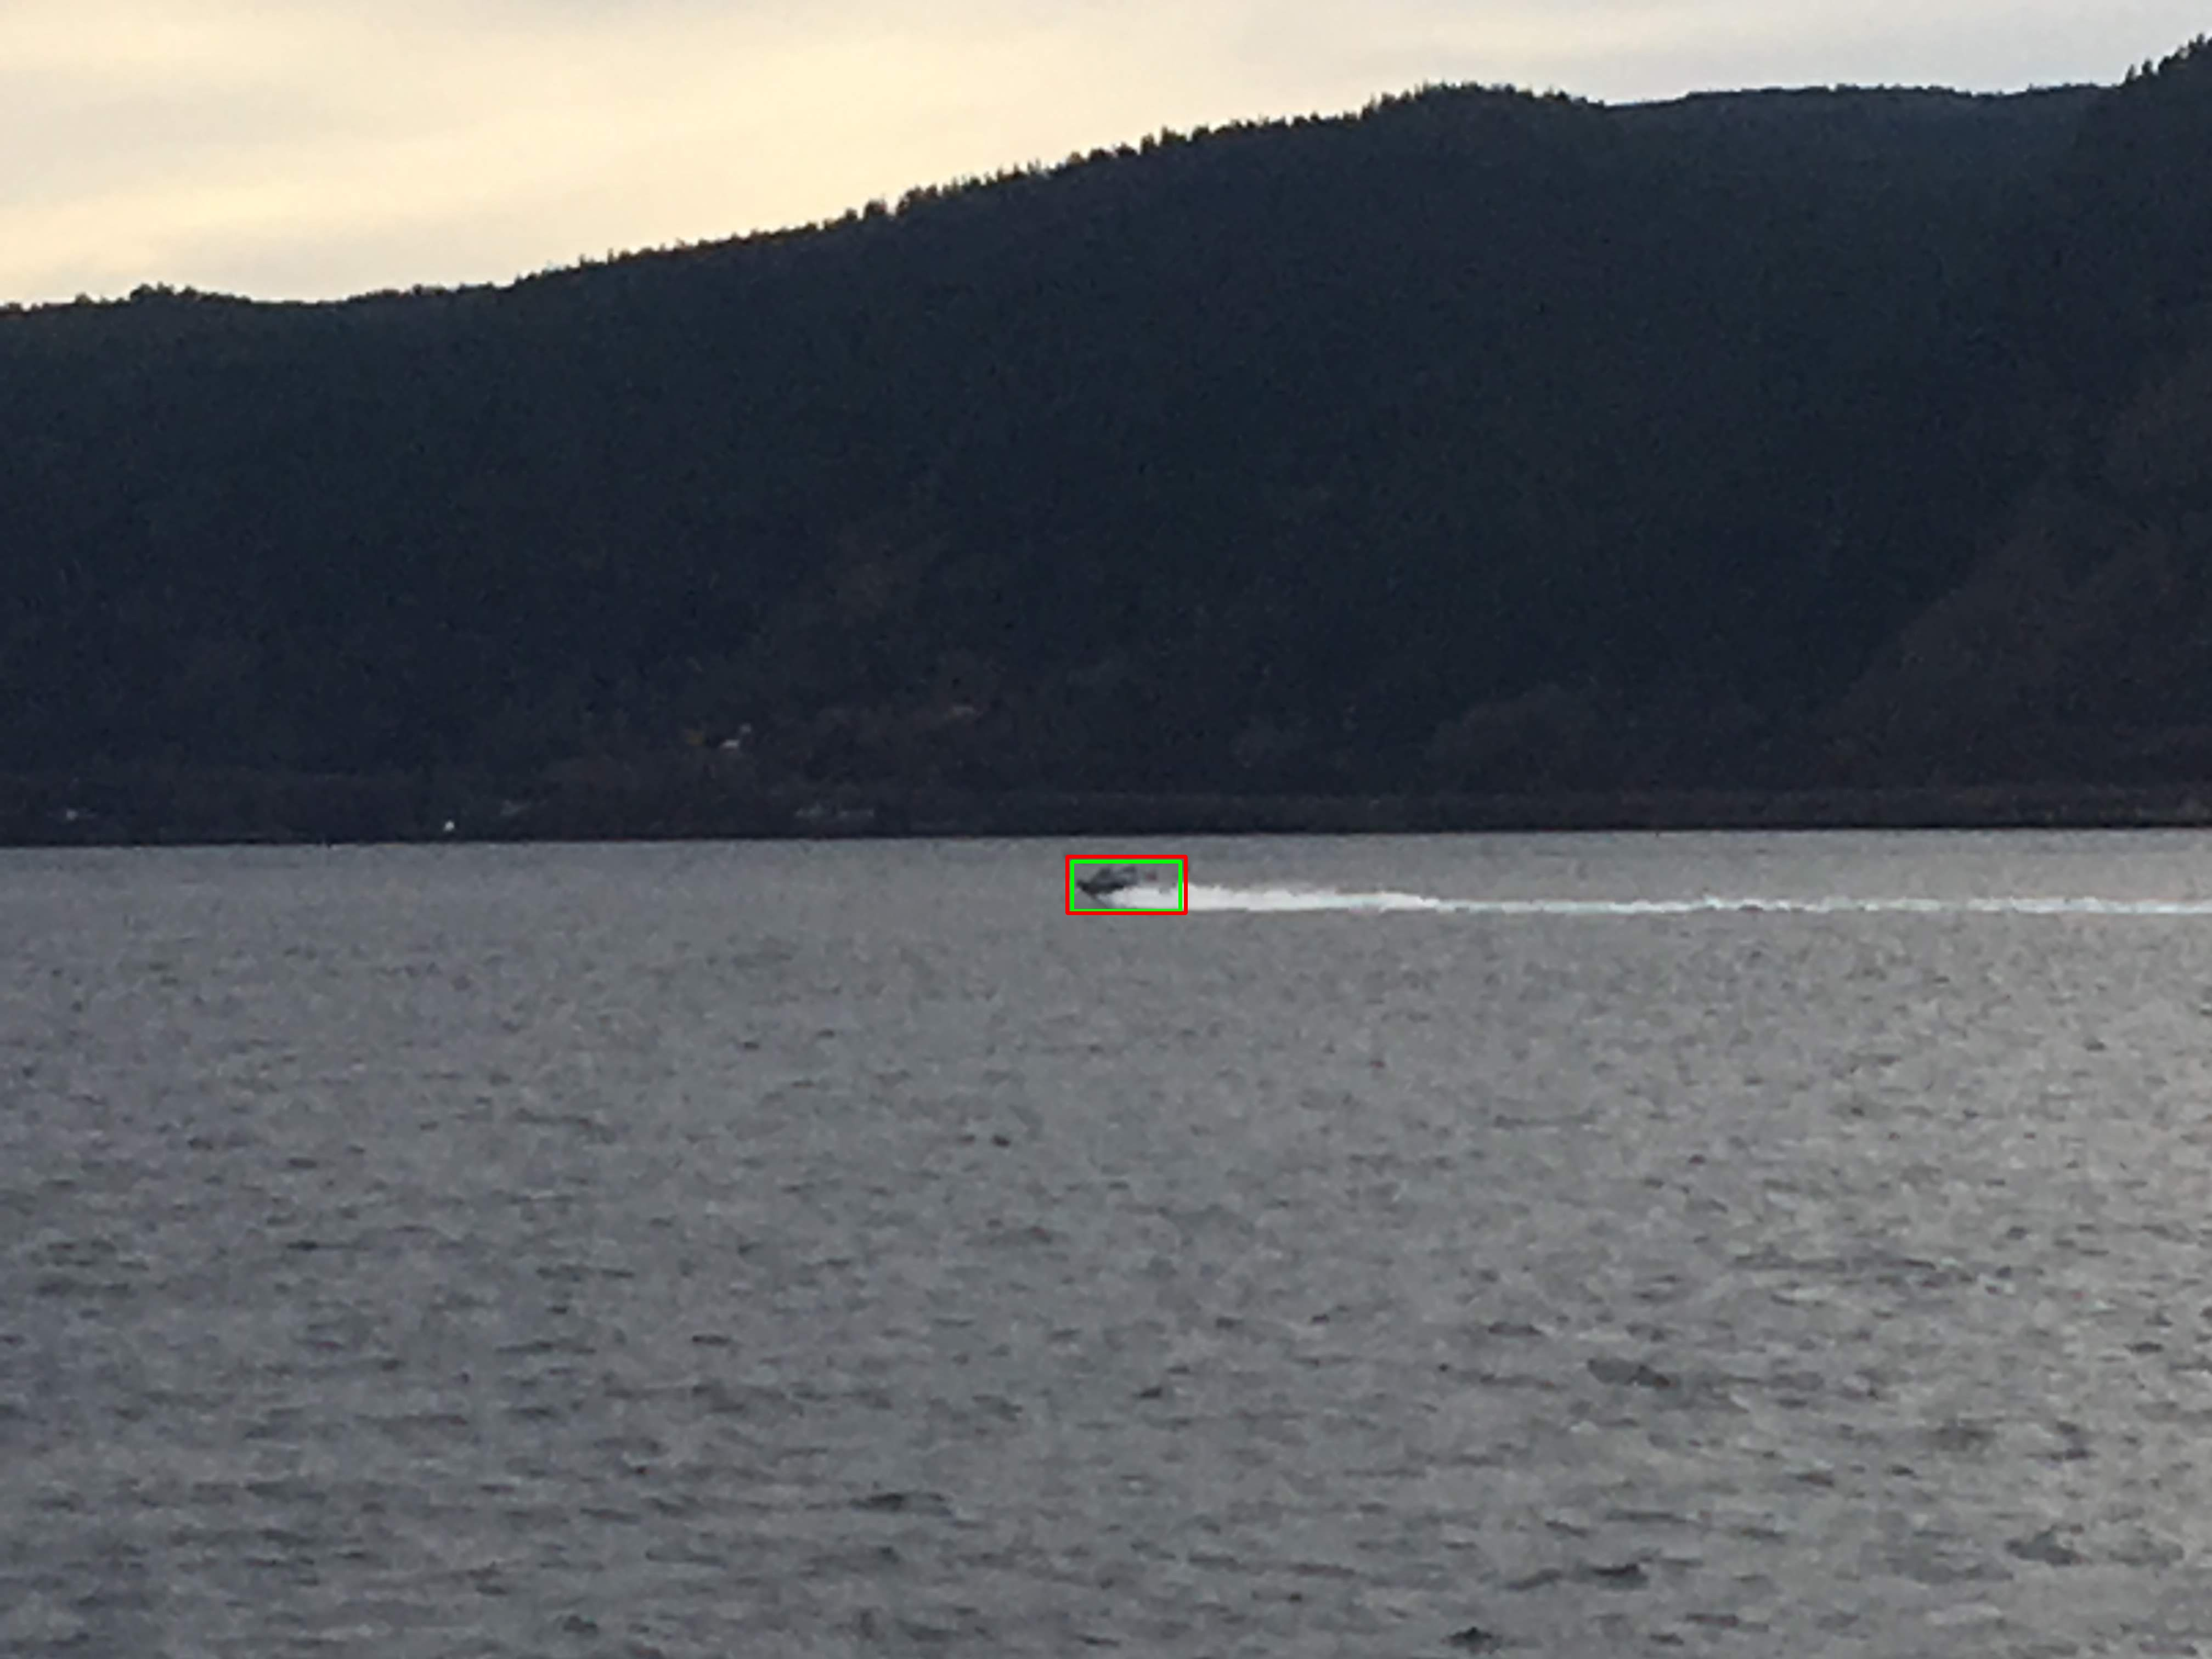
\includegraphics[width=.8\linewidth]{results/case_buildings/ssdtrf/ssd3/grov2/IMG_2325.jpg}
  \caption{SSD3}
  \label{fig:ex_trf_prec_rec_ssd}
\end{subfigure}
\caption{SSD2 and SSD3 example image}
\label{fig:ssd_trf_bigbox}
\end{figure}

There are examples where SSD2 detects boats correctly while SSD3 don't and vice versa. For example images of this behaviour see Appendix C, chapter \ref{sec_ssd3_better_trf} and \ref{sec_ssd2_better_trf}. In a few test images, SSD3 wrongly classifies buildings as boats, while SSD2 does not. This is counter-intuitive since the idea behind training SSD3 on buildings was to make it suppress these detections. An example of this is shown in figure \ref{fig:ssd3_misclassify}.

\begin{figure}[h!]
\begin{subfigure}{.5\textwidth}
  \centering
  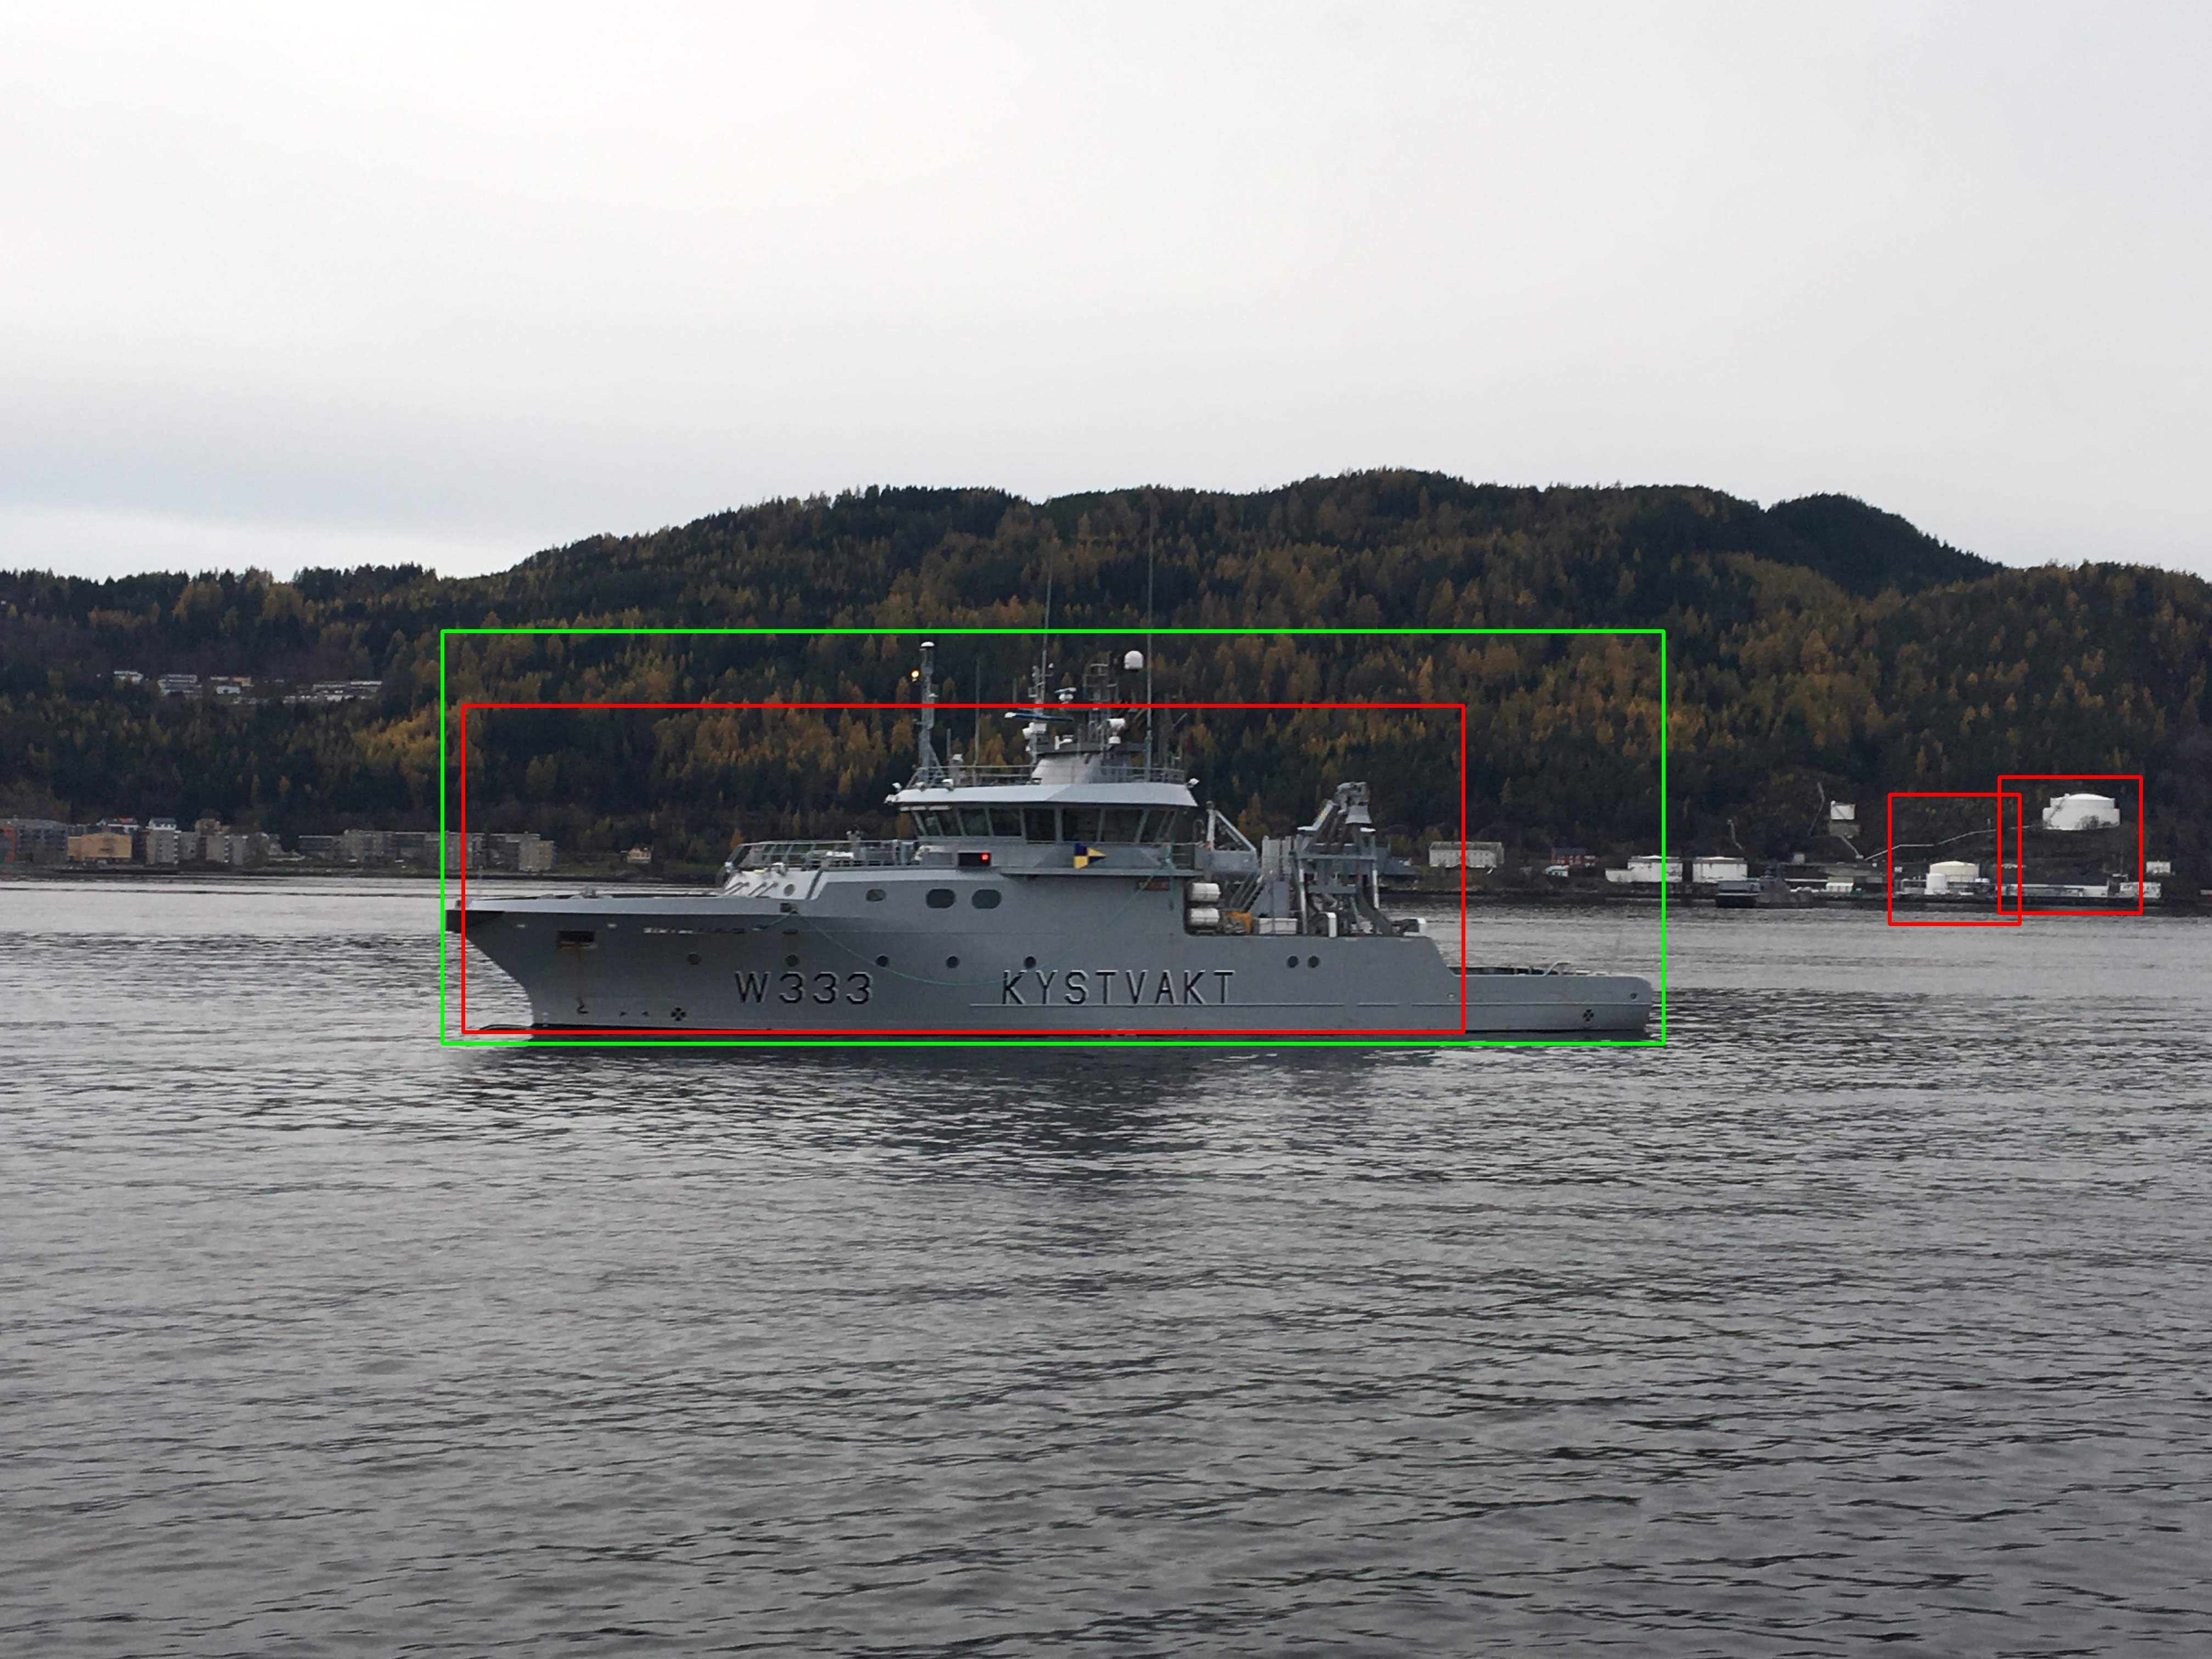
\includegraphics[width=0.8\linewidth]{results/case_buildings/ssdtrf/ssd2/grov3/IMG_2680.jpg}
  \caption{SSD2}
  \label{fig:ex_trf_prec_rec_yolo}
\end{subfigure}%
\begin{subfigure}{.5\textwidth}
  \centering
  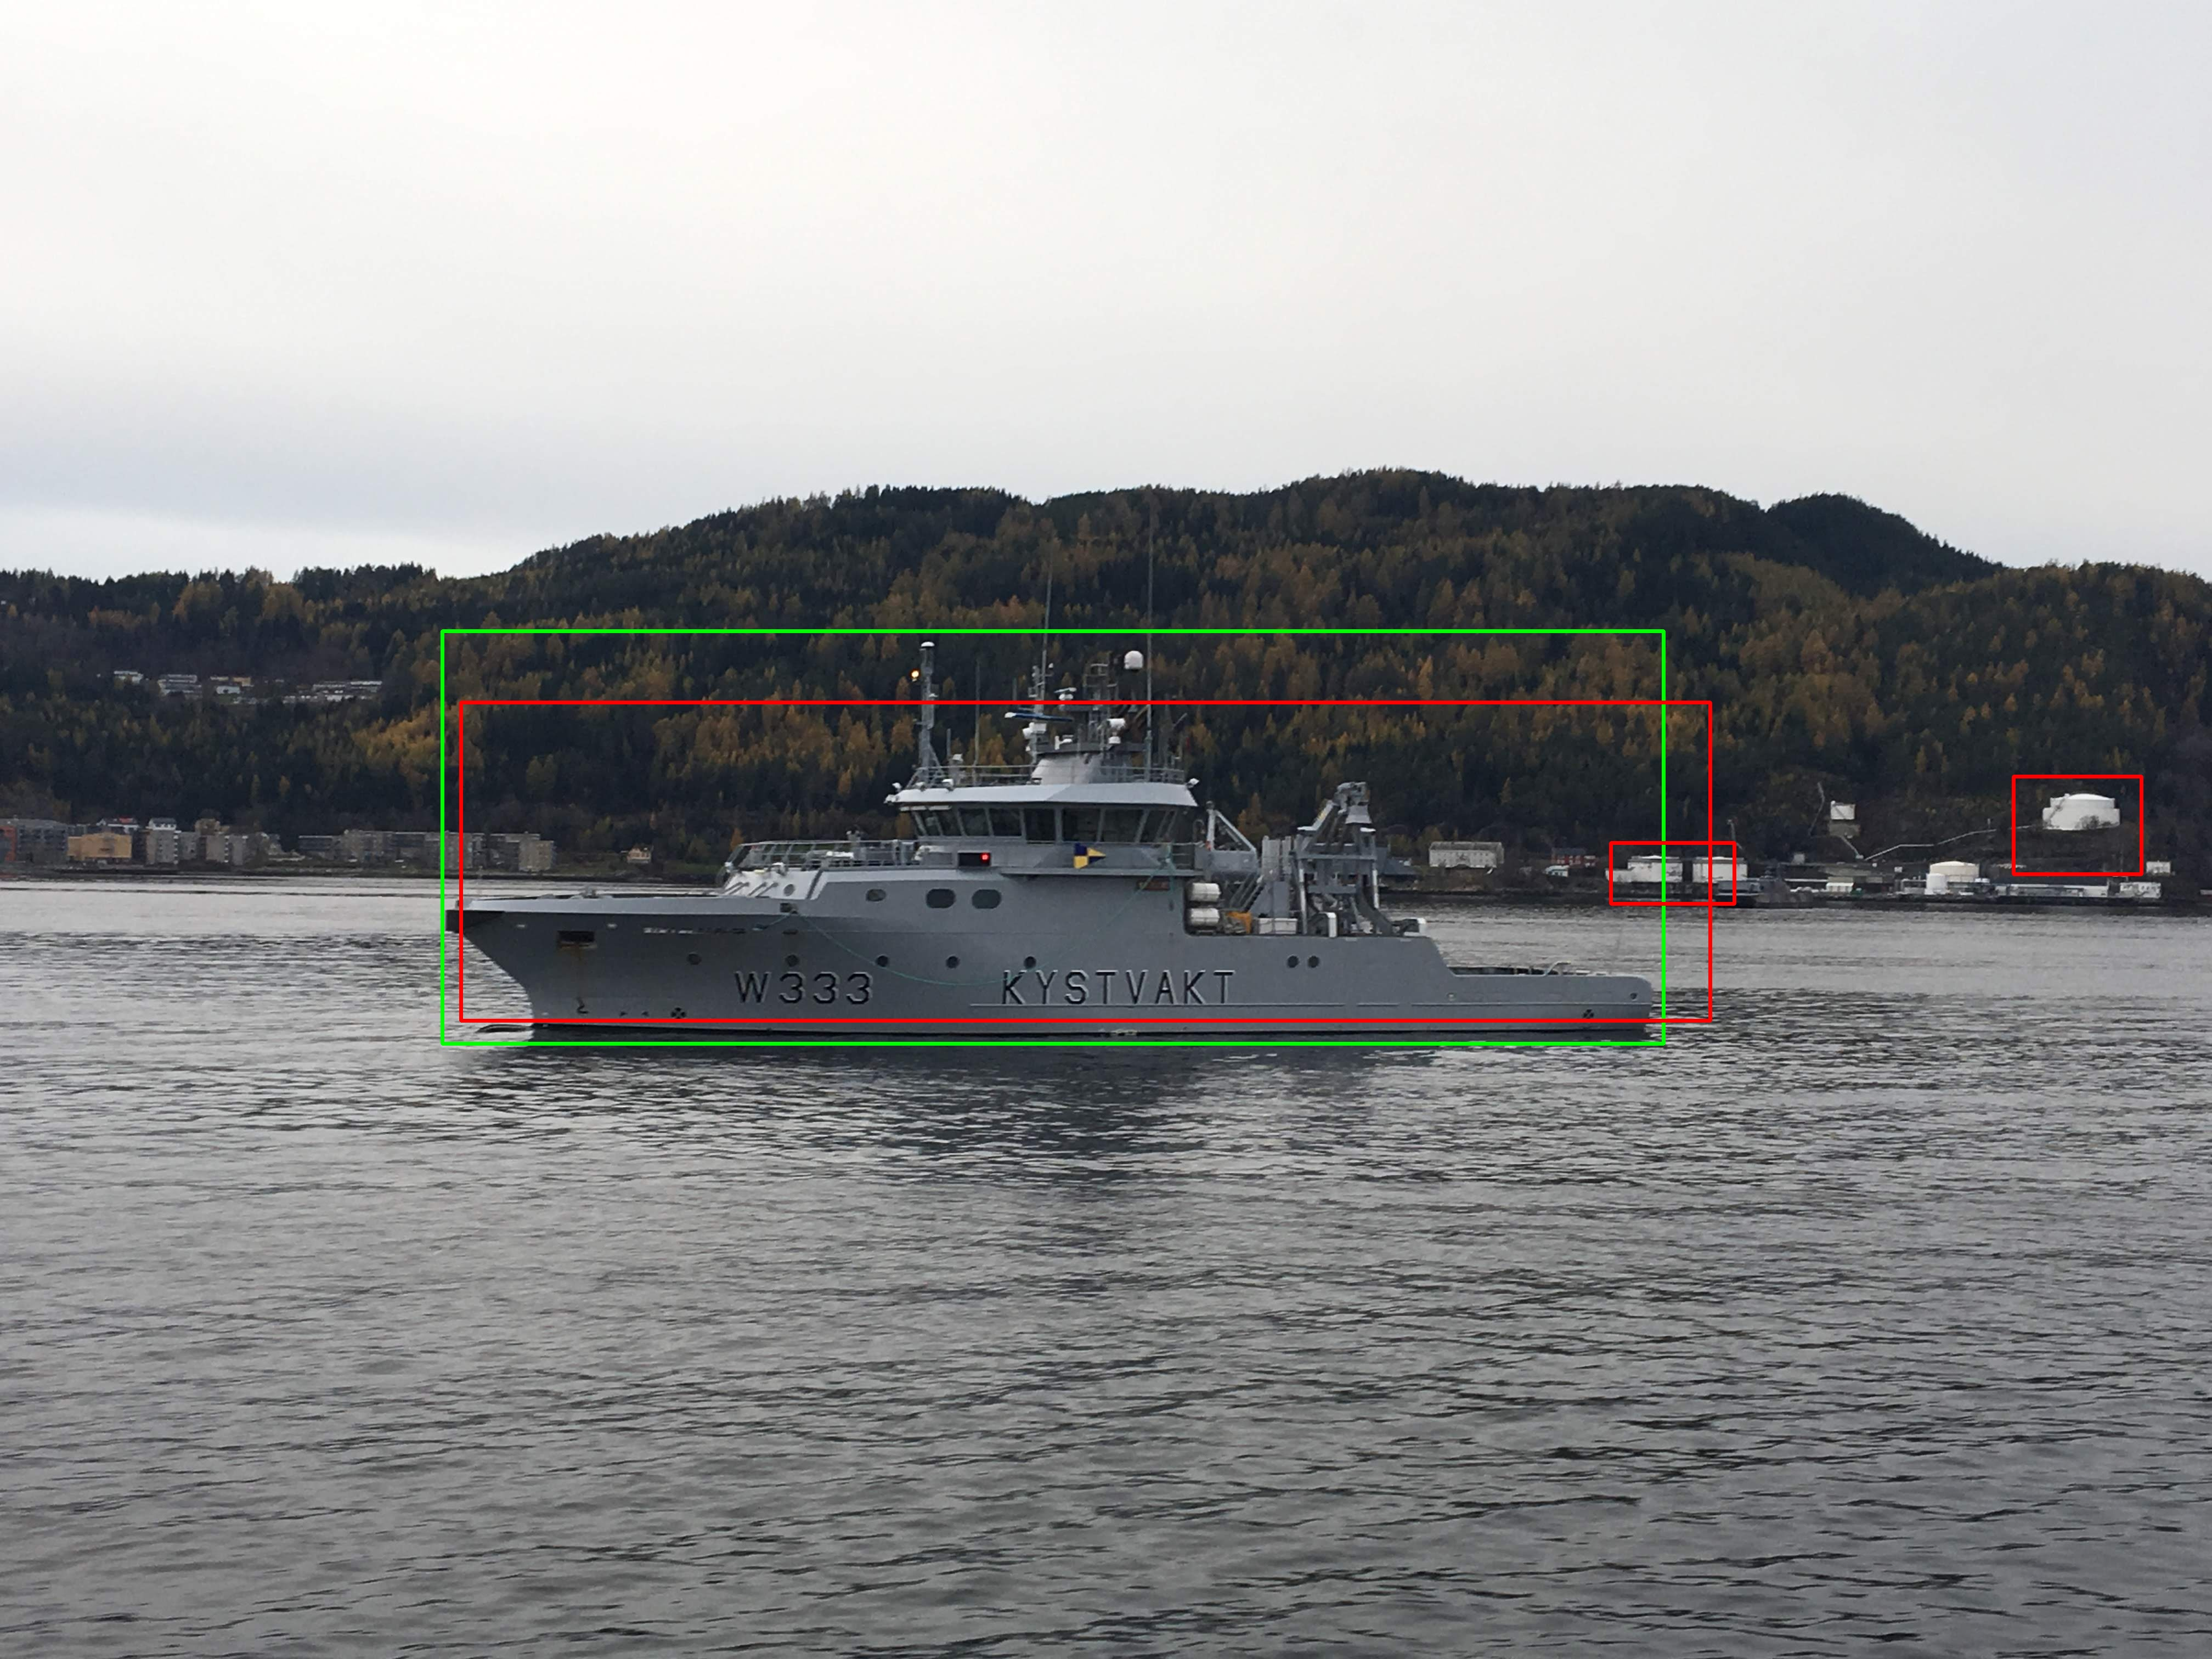
\includegraphics[width=.8\linewidth]{results/case_buildings/ssdtrf/ssd3/grov3/IMG_2680.jpg}
  \caption{SSD3}
  \label{fig:ex_trf_prec_rec_ssd}
\end{subfigure}
\caption{SSD3 misclassifies two buildings as boats}
\label{fig:ssd3_misclassify}
\end{figure}

In this figure \ref{fig:ssd3_misclassify} SSD3 does not detect the buildings as buildings, this will be discussed further in chapter \ref{sec:build_trf}.

\vspace{3mm}

\subsubsection{Yolo2 and Yolo3 on trf}

Yolo2 and Yolo3 both have outstanding results on trf, but Yolo2 has a few misclassifications that Yolo3 does not have. In figure \ref{fig:yolo2_misclassify} Yolo2 detects land as a boat, and in figure \ref{fig:Yolo3_better_trf} Yolo3 detects a boat that Yolo2 does not. There are not many examples where their performance differs much, but there are a few which makes Yolo3 a little more robust than Yolo2.

\begin{figure}[h!]
\begin{subfigure}{.5\textwidth}
  \centering
  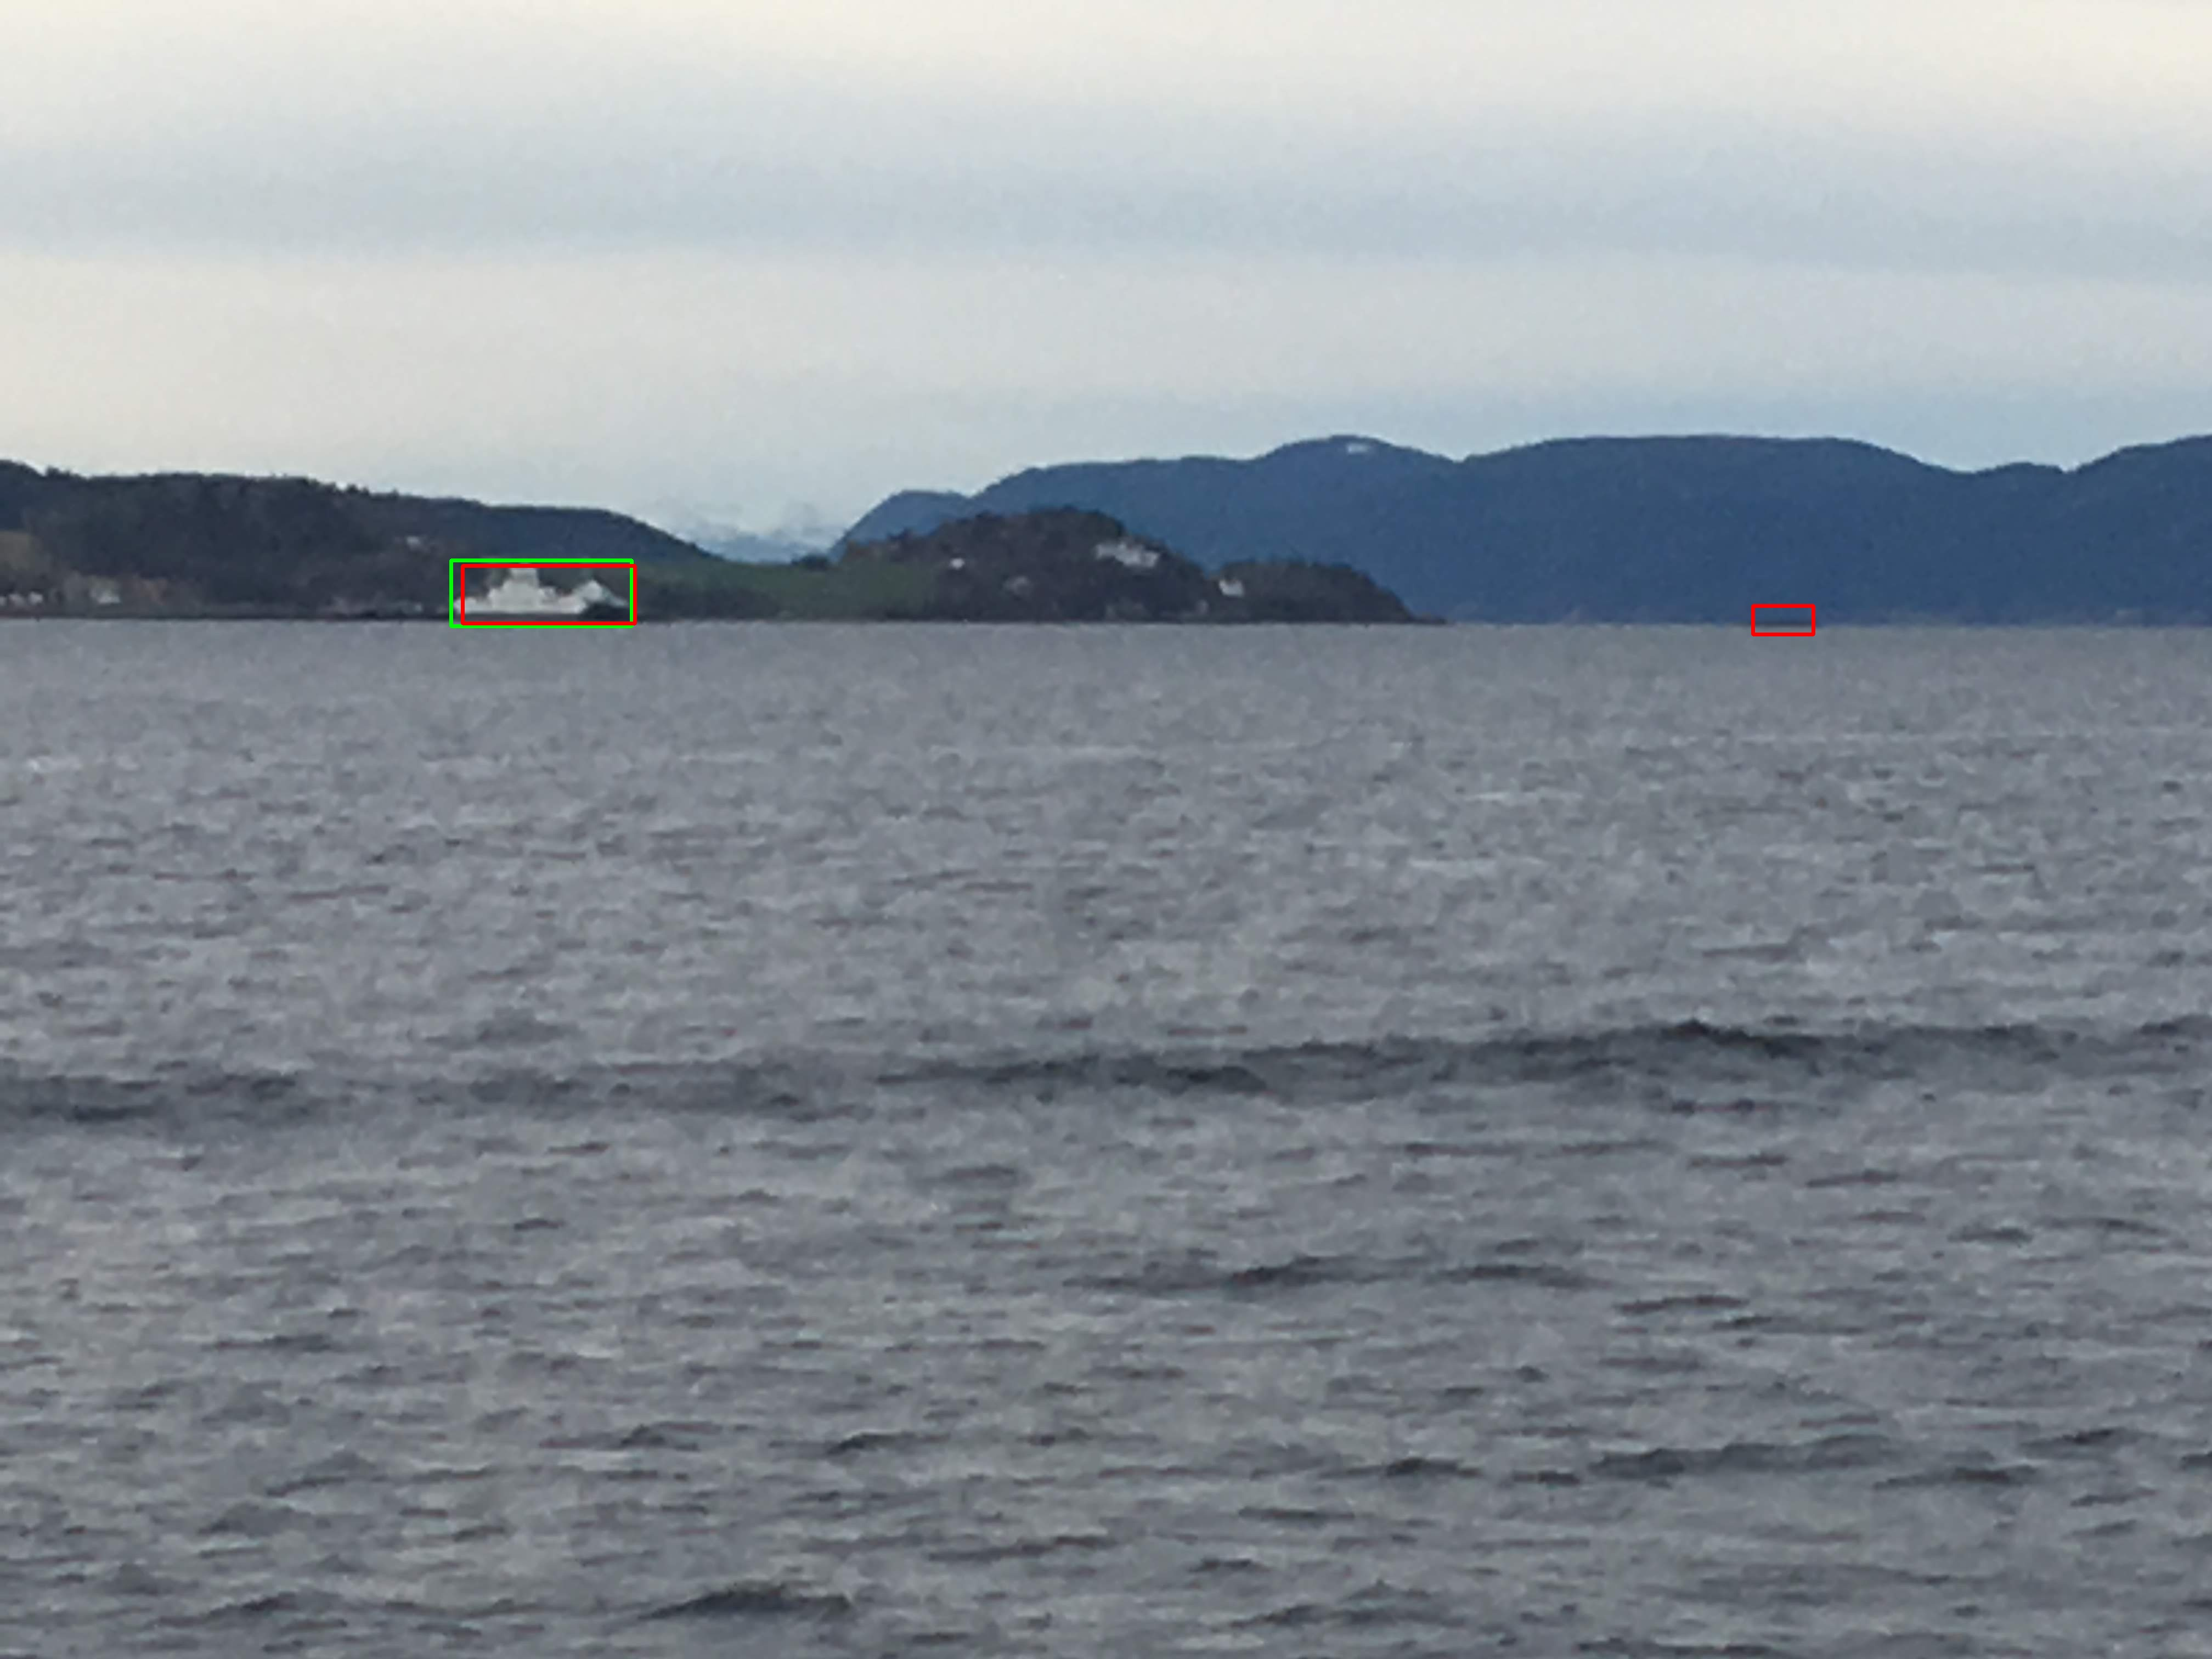
\includegraphics[width=0.8\linewidth]{results/case_buildings/yolotrf/Yolo2/IMG_2300.jpg}
  \caption{Yolo2}
  %\label{fig:ex_trf_prec_rec_yolo}
\end{subfigure}%
\begin{subfigure}{.5\textwidth}
  \centering
  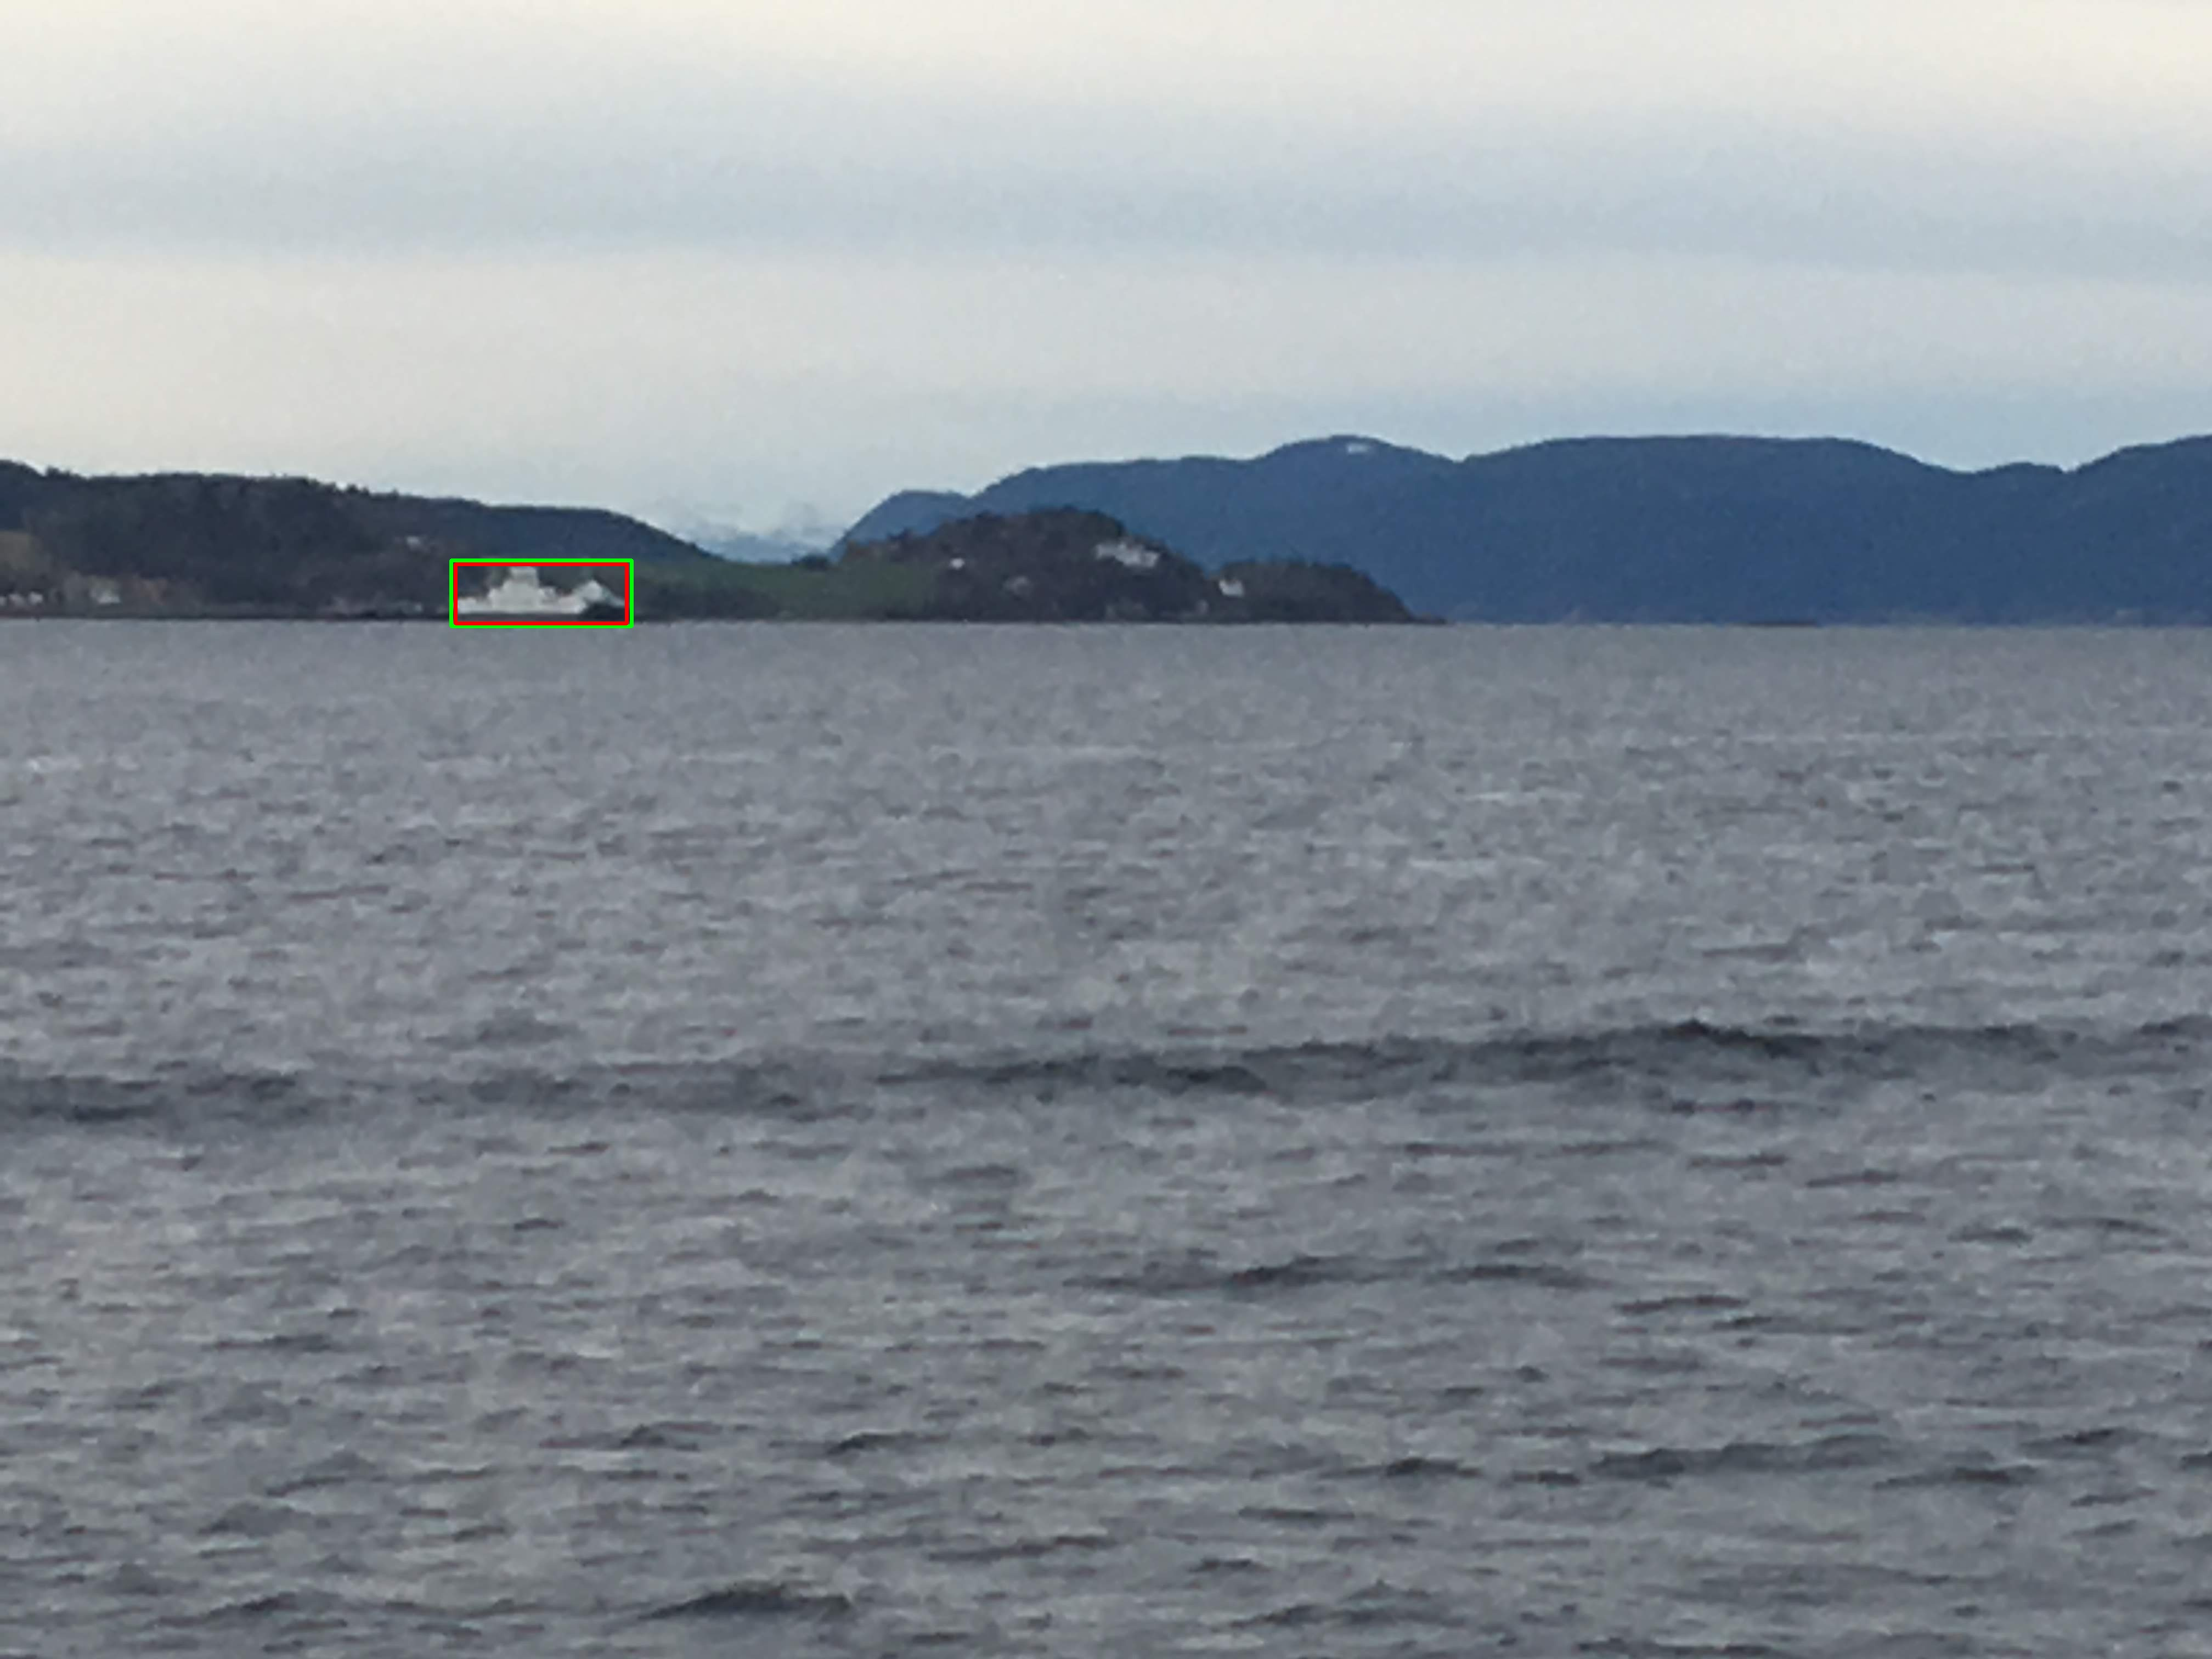
\includegraphics[width=.8\linewidth]{results/case_buildings/yolotrf/Yolo3/IMG_2300.jpg}
  \caption{Yolo3}
  %\label{fig:ex_trf_prec_rec_ssd}
\end{subfigure}
\caption{Yolo2 misclassifies land as boat}
\label{fig:yolo2_misclassify}
\end{figure}

\begin{figure}[h!]
\begin{subfigure}{.5\textwidth}
  \centering
  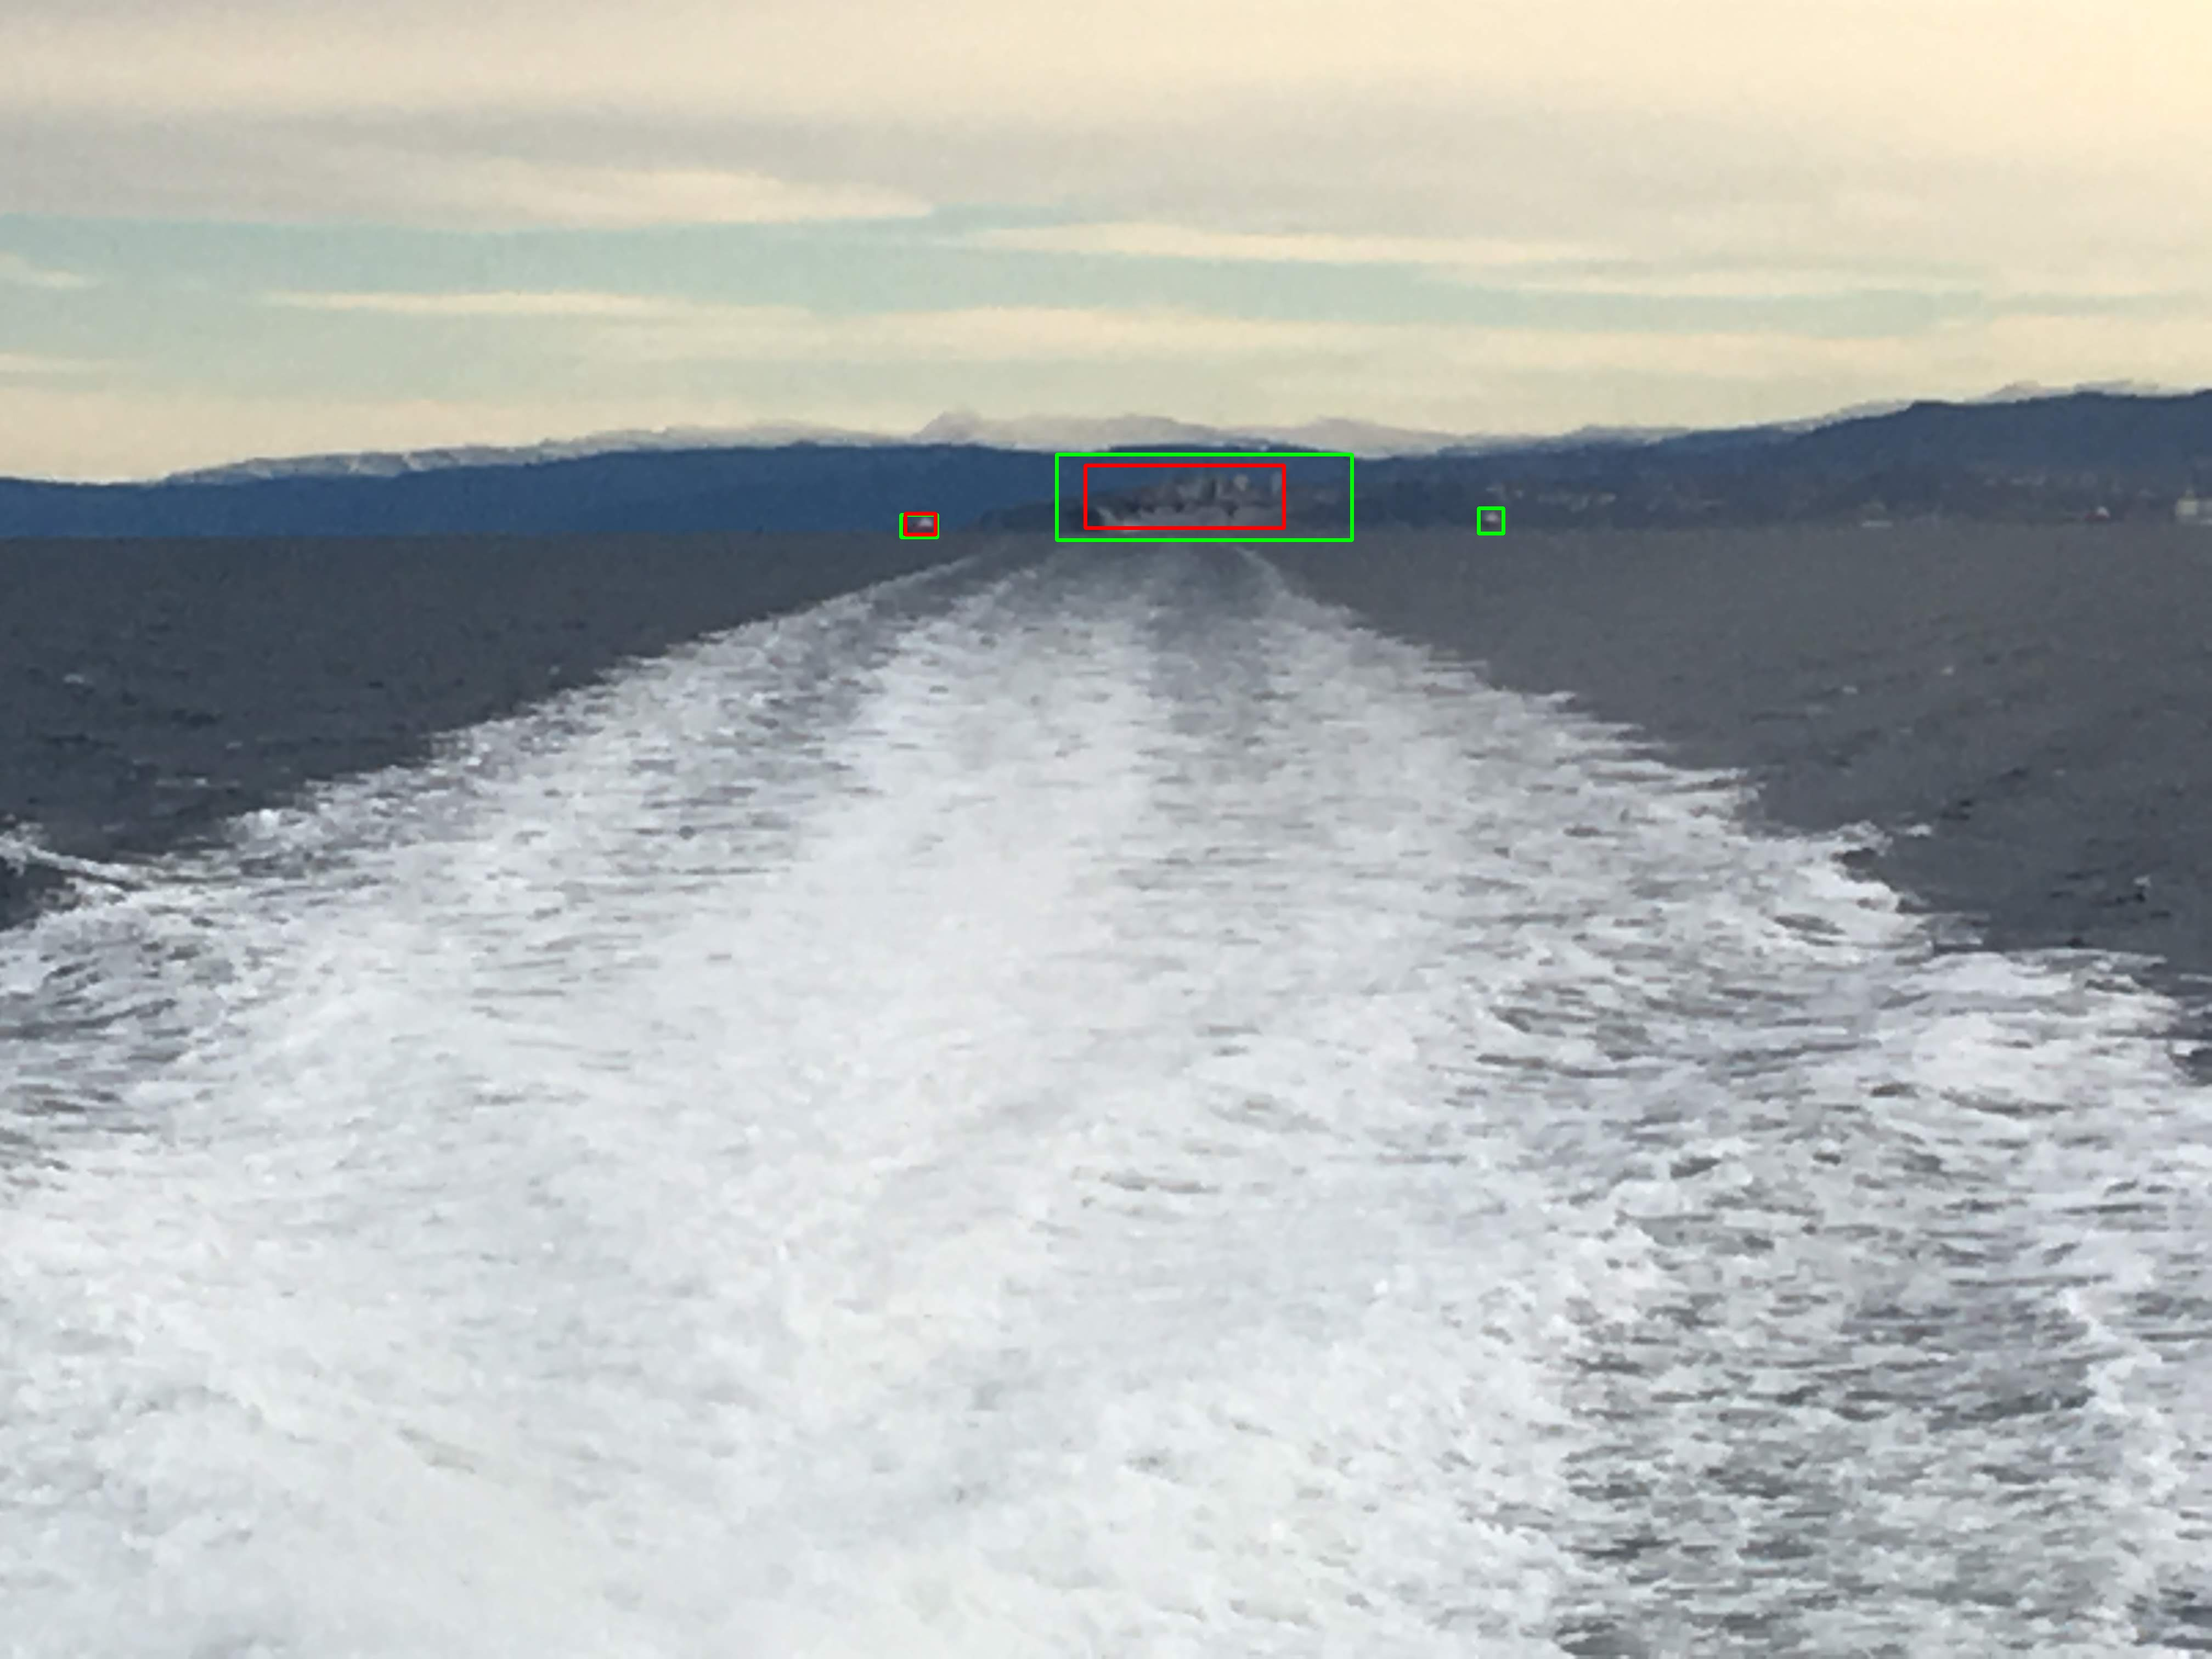
\includegraphics[width=0.8\linewidth]{results/case_buildings/yolotrf/Yolo2/IMG_2350.jpg}
  \caption{Yolo2}
  %\label{fig:ex_trf_prec_rec_yolo}
\end{subfigure}%
\begin{subfigure}{.5\textwidth}
  \centering
  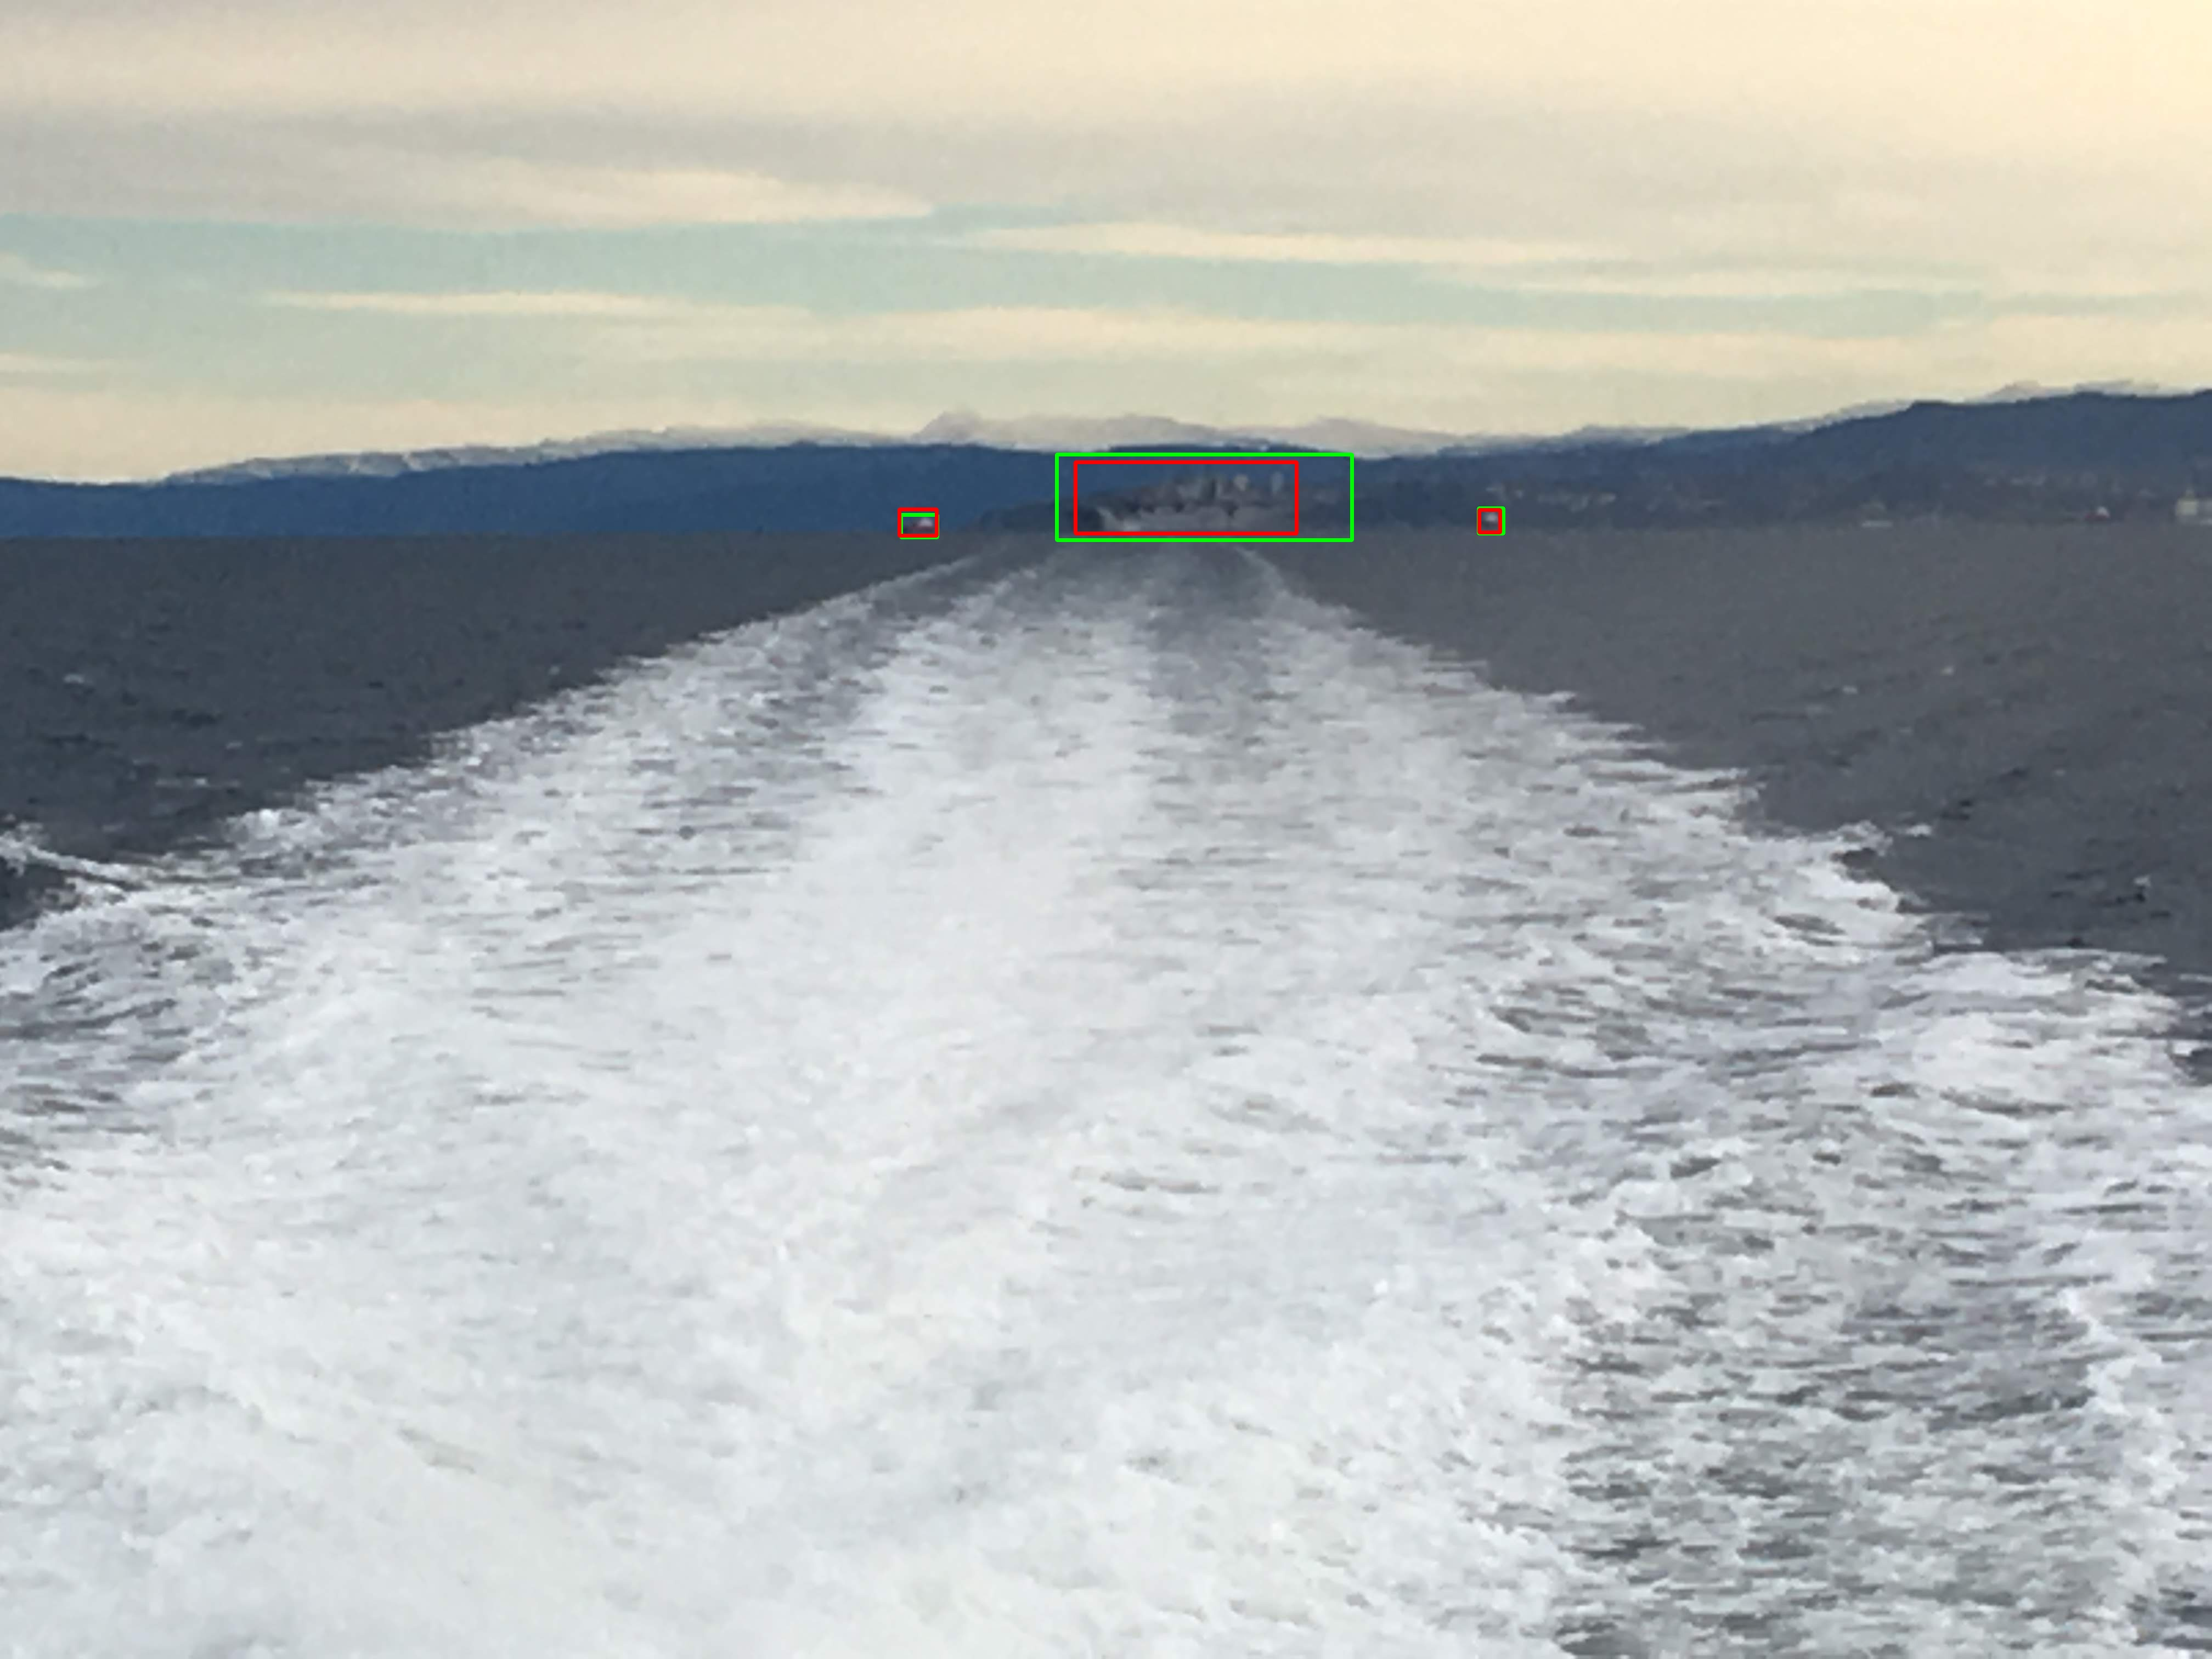
\includegraphics[width=.8\linewidth]{results/case_buildings/yolotrf/Yolo3/IMG_2350.jpg}
  \caption{Yolo3}
  %\label{fig:ex_trf_prec_rec_ssd}
\end{subfigure}
\caption{Yolo2 does not detect rightmost boat, Yolo3 does}
\label{fig:Yolo3_better_trf}
\end{figure}

\newpage
\clearpage

\section{Effect of training on moored boats testing for sailing boats}

Since Yolo3's results on trf are nearly perfect, as shown in figure \ref{fig:moor_trf} and suspicion of overtraining was raised, a case-study of how training on moored boats (bbnb) affect the results on detection of sailing boats (bc, bf, trf), was done. Since Yolo2's and Yolo3's results on trf are better than Yolo1's, without more training on the same data, it could imply that the good results are not connected to overtraining. This will be further discussed in \ref{dataset_divers}.


\begin{figure}[h!]
\begin{subfigure}{.5\textwidth}
  \centering
  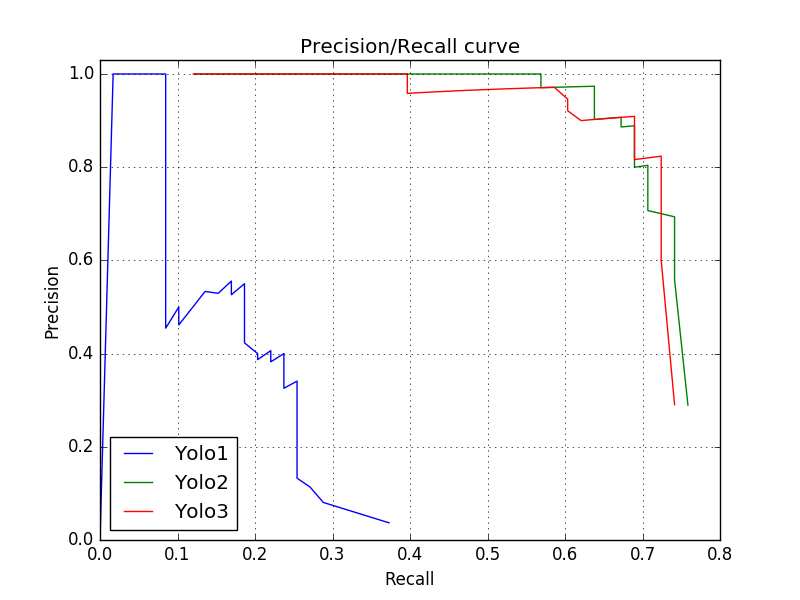
\includegraphics[width=0.8\linewidth]{results/case_tr_moor/prec_recall/bb.png}
  \caption{Yolo1, Yolo2 and Yolo3 on bbnb}
  \label{fig:moor_bb}
\end{subfigure}%
\begin{subfigure}{.5\textwidth}
  \centering
  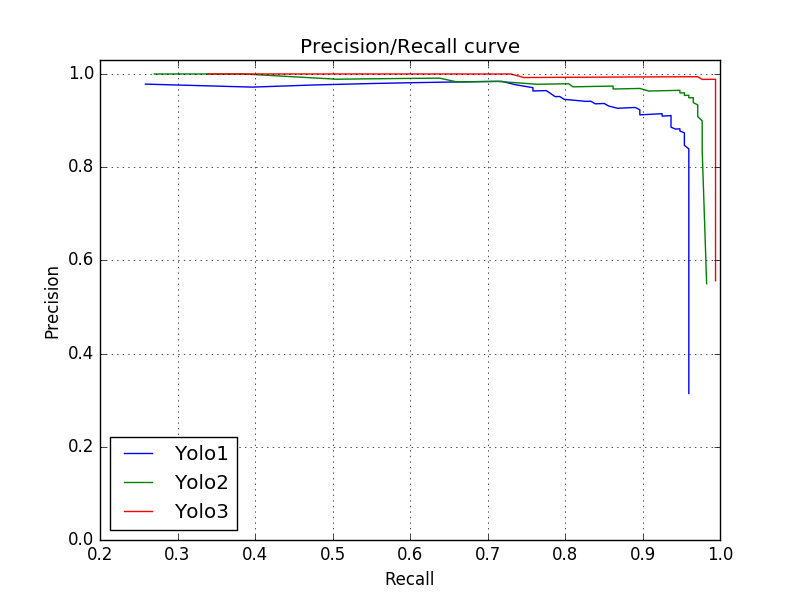
\includegraphics[width=.8\linewidth]{results/case_tr_moor/prec_recall/trf.png}
  \caption{Yolo1, Yolo2 and Yolo3 on trf}
  \label{fig:moor_trf}
\end{subfigure}

\begin{subfigure}{.5\textwidth}
  \centering
  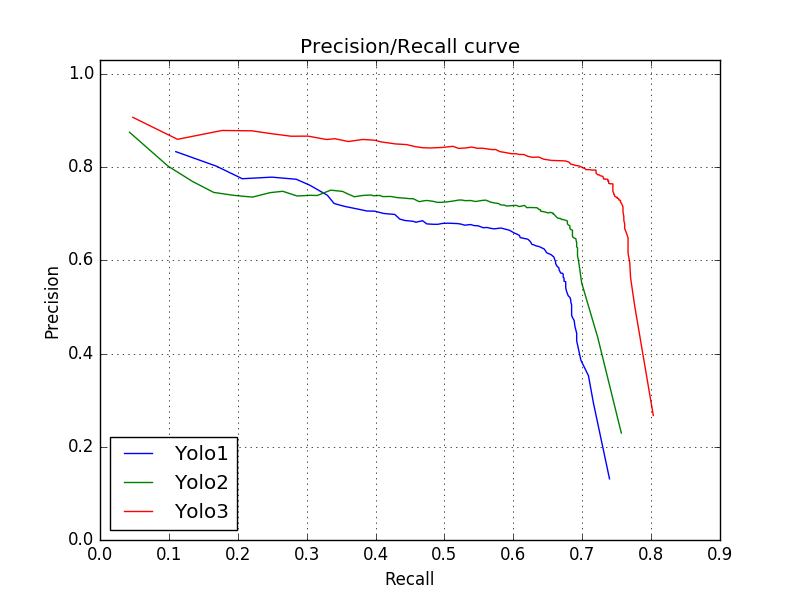
\includegraphics[width=0.8\linewidth]{results/case_tr_moor/prec_recall/bcbf.png}
  \caption{Yolo1, Yolo2 and Yolo3 on bc, bf}
  %\label{fig:moor_bcbf}
\end{subfigure}%
\begin{subfigure}{.5\textwidth}
  \centering
  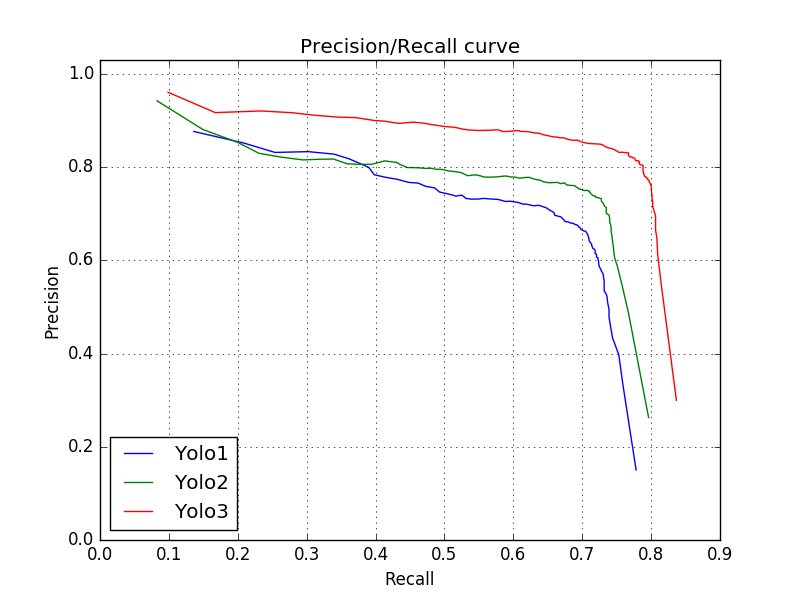
\includegraphics[width=.8\linewidth]{results/case_tr_moor/prec_recall/bcbftrf.png}
  \caption{Yolo1, Yolo2 and Yolo3 on bc, bf, trf}
  %\label{fig:moor_bcbftrf}
\end{subfigure}
\caption{Precision/recall curves for Yolo1, Yolo2, SSD1 and SSD2 on bb and on bc, bf, trf}
\label{fig:prec_rec_case_moor}

\end{figure}

In figure \ref{fig:prec_rec_case_moor} the precision/recall curves for Yolo1, Yolo2 and Yolo3 are plotted. In all the test cases are Yolo2 and Yolo3 better than Yolo1. While this is expected behavior when testing on bbnb, the results are not intuitive for the other test cases. 

\vspace{3mm}

Two clear differences between Yolo1 and Yolo2 were found while analyzing the results. The first one being that Yolo1 tends to overestimate the size of large ships, as shown in figure \ref{fig:yolo12_big}. More examples of this behavior can be seen in Appendix C, chapter \ref{sec:yolo1_big_box}

\begin{figure}[h!]
\begin{subfigure}{.5\textwidth}
  \centering
  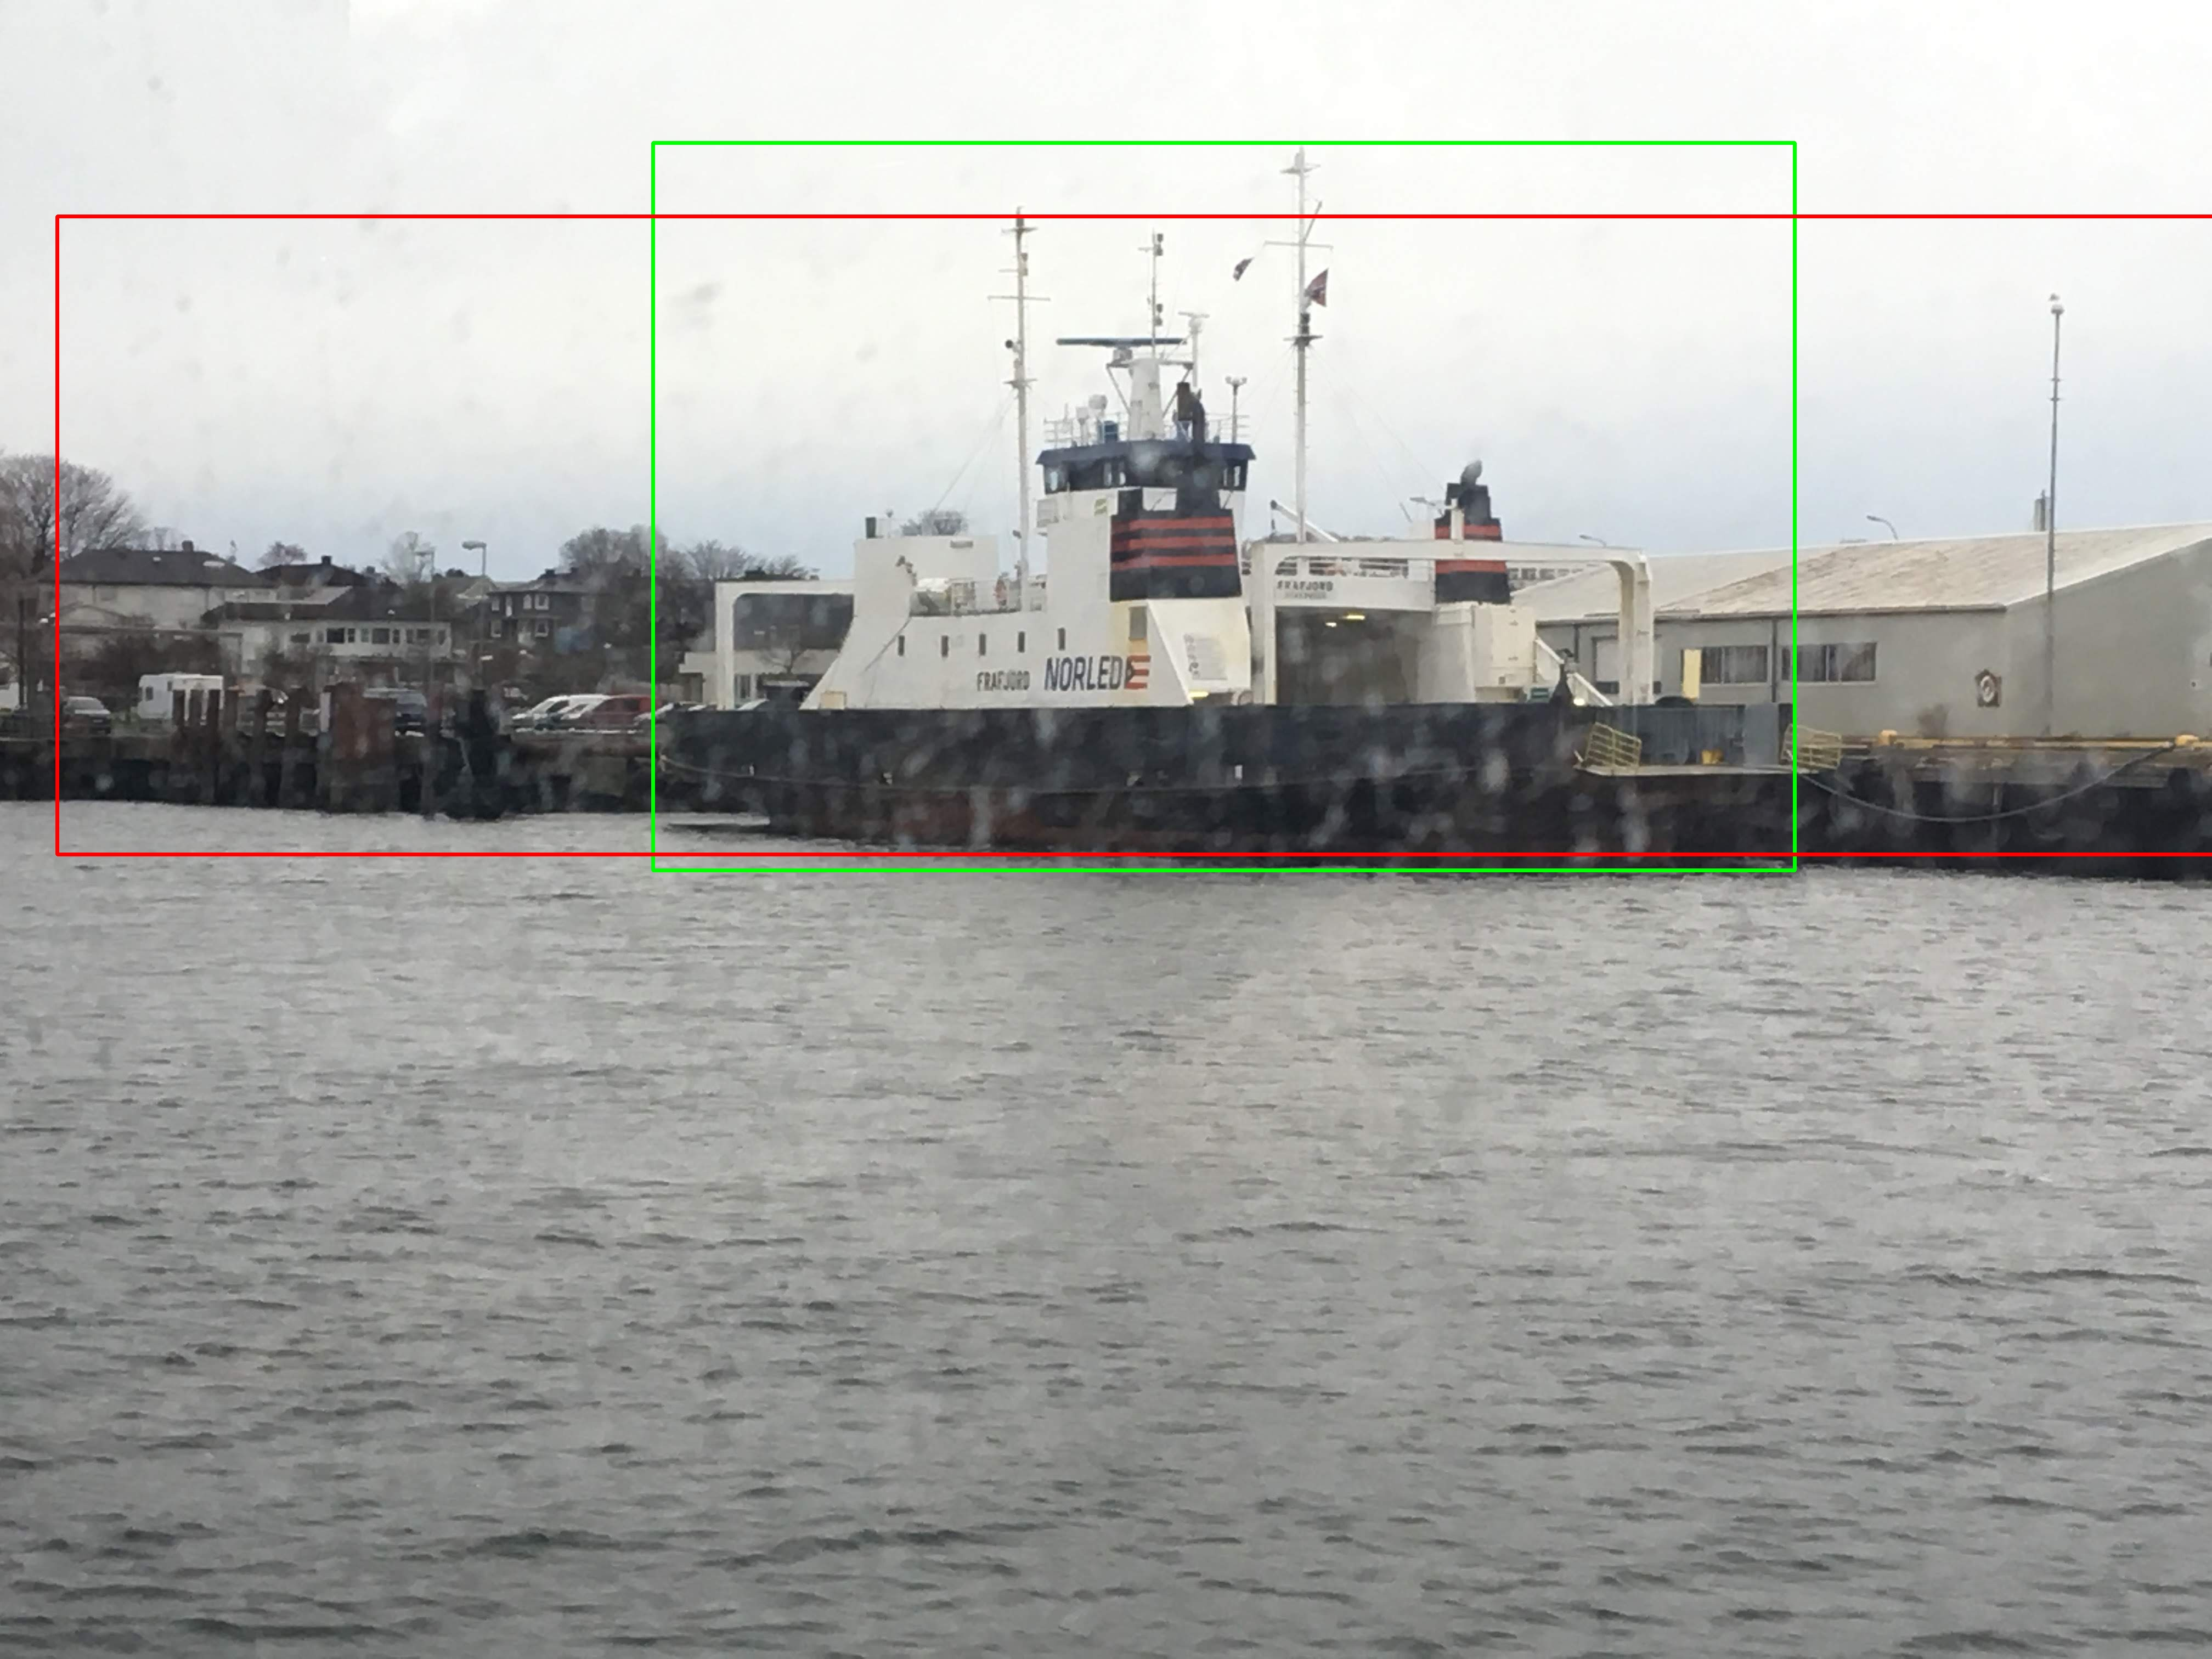
\includegraphics[width=0.8\linewidth]{results/case_tr_moor/yolo12/yolo1/big/IMG_2566.jpg}
  \caption{Yolo1}
  \label{fig:yolo1_big}
\end{subfigure}%
\begin{subfigure}{.5\textwidth}
  \centering
  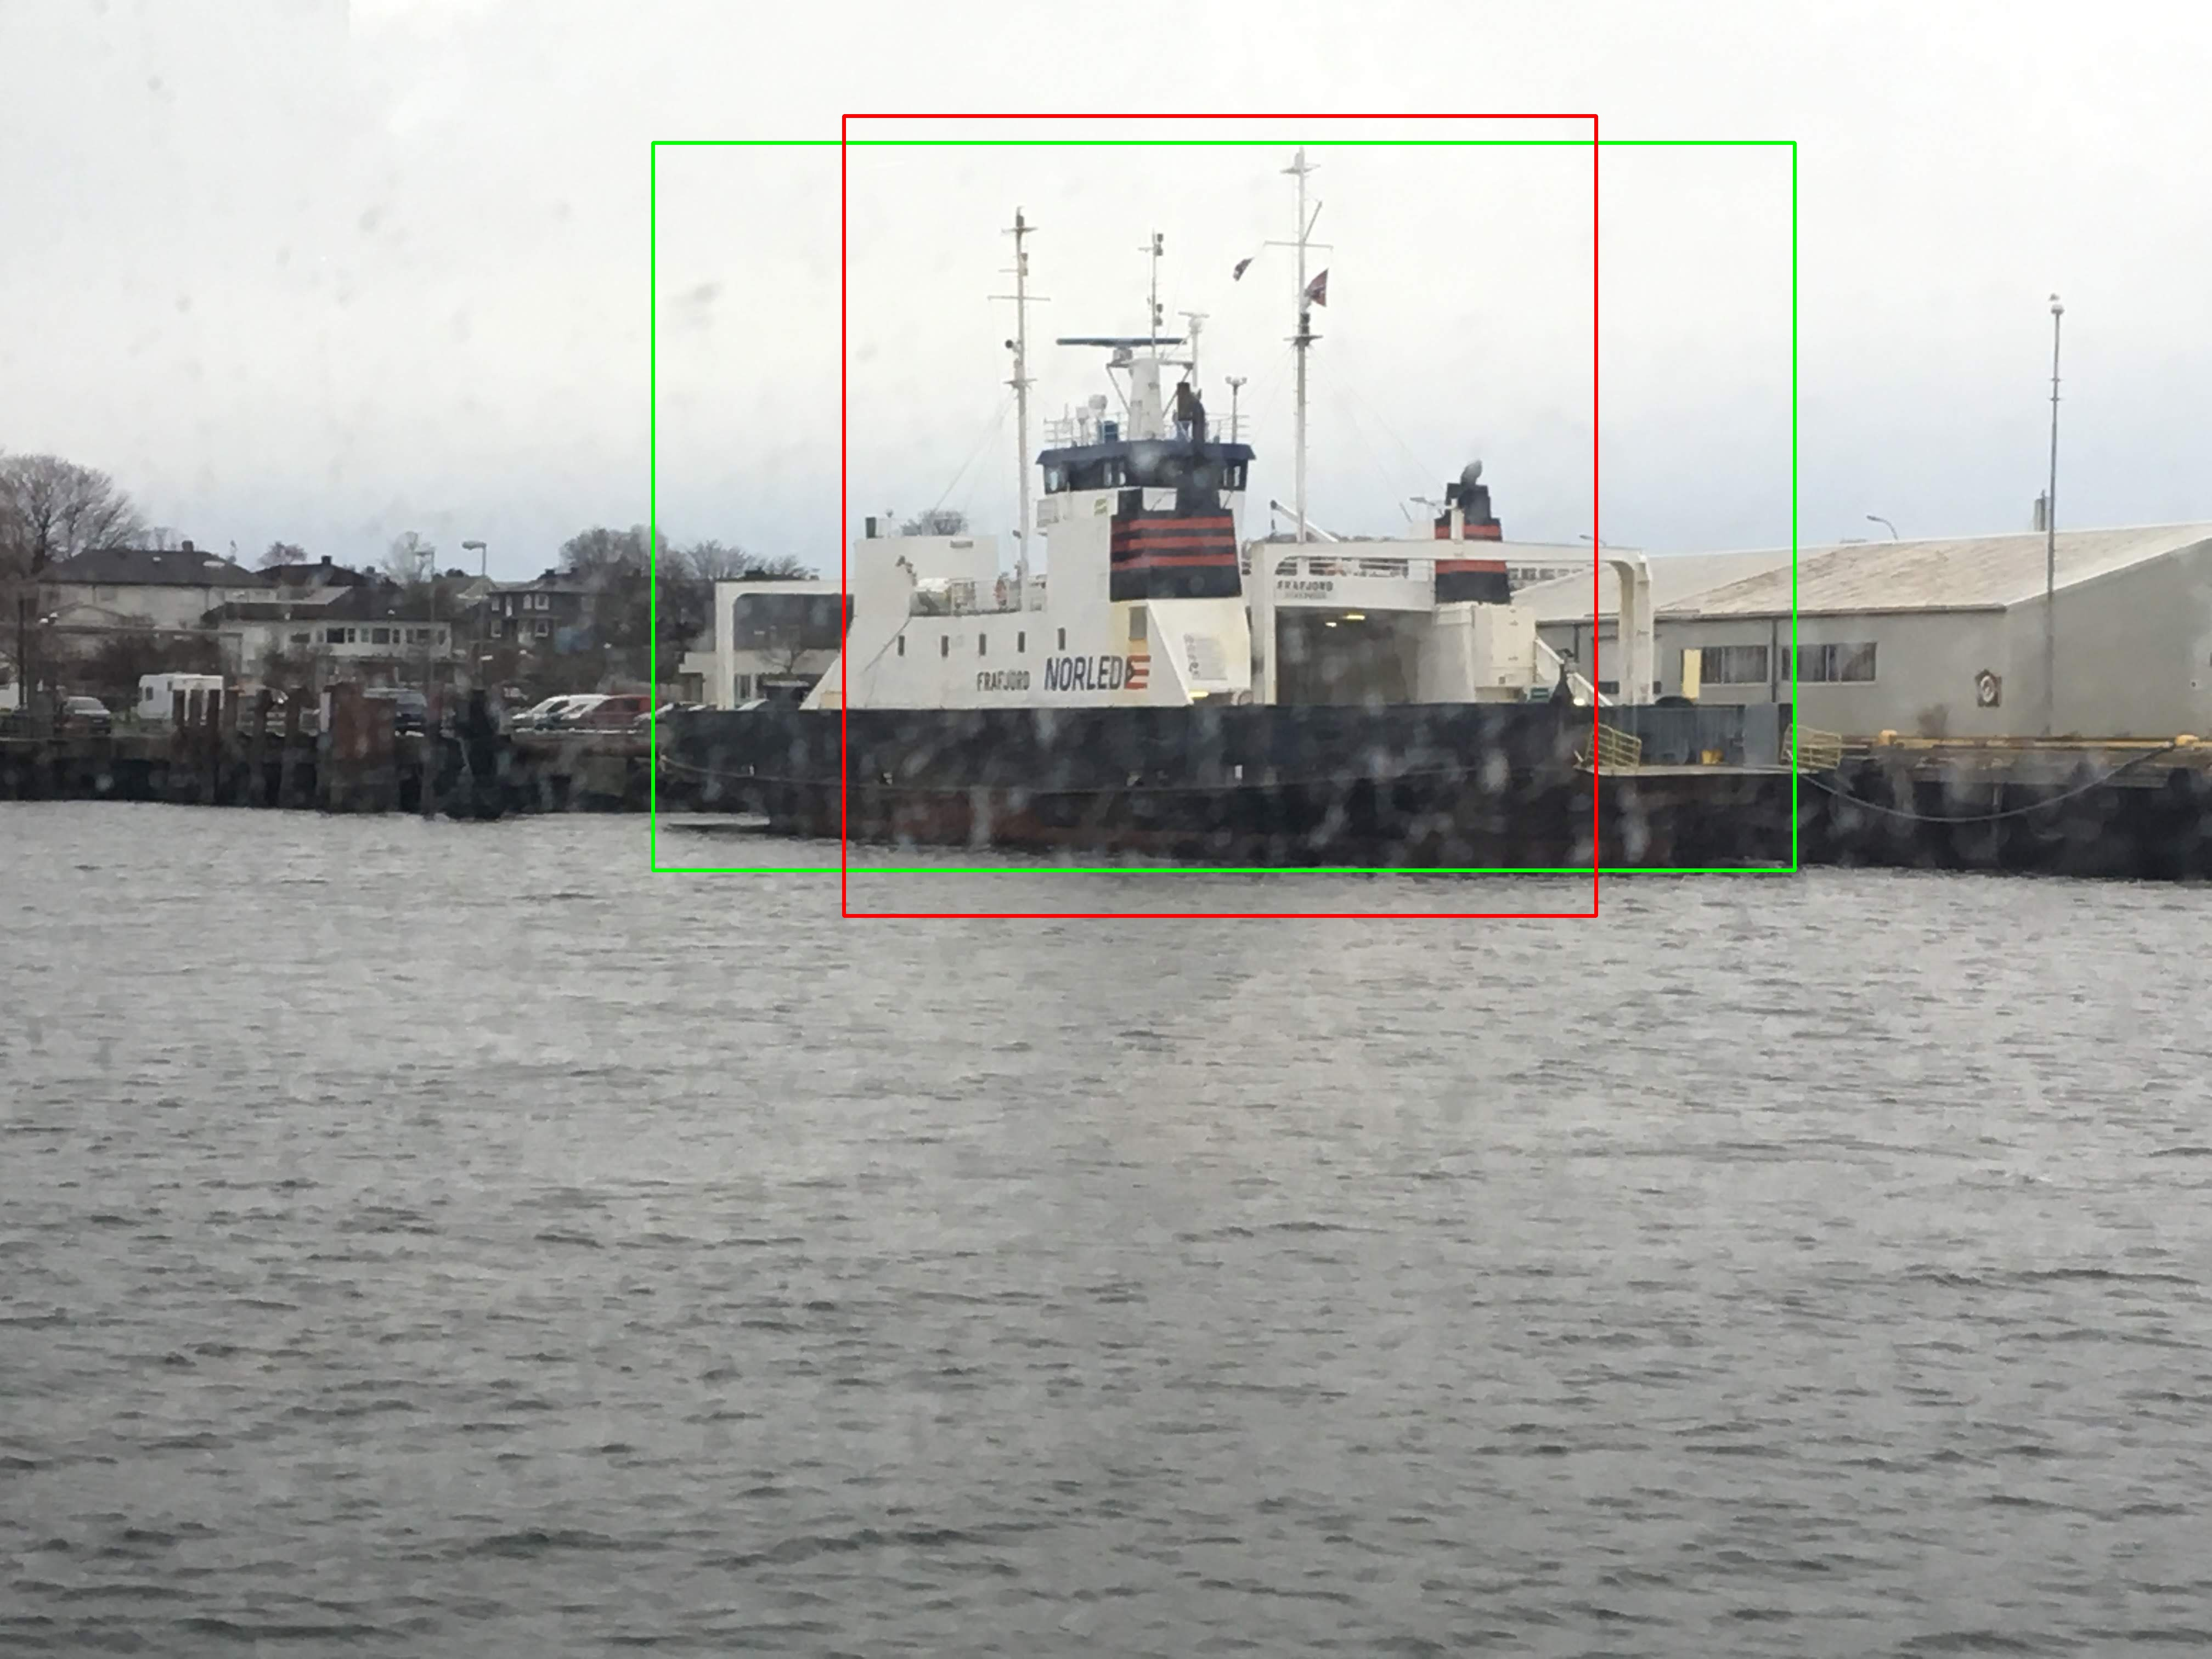
\includegraphics[width=.8\linewidth]{results/case_tr_moor/yolo12/yolo2/big/IMG_2566.jpg}
  \caption{Yolo2}
  \label{fig:yolo2_big}
\end{subfigure}
\caption{Example of Yolo1 over estimating size of ship}
\label{fig:yolo12_big}
\end{figure}

\newpage

Yolo1 also has a penchant to detect the same boat twice, where Yolo2 does not, as shown in figure \ref{fig:yolo12_multibox}. More examples of this behavior are shown in Appendix C, chapter \ref{sec:yolo1_multidetect}.

\begin{figure}[h!]
\begin{subfigure}{.5\textwidth}
  \centering
  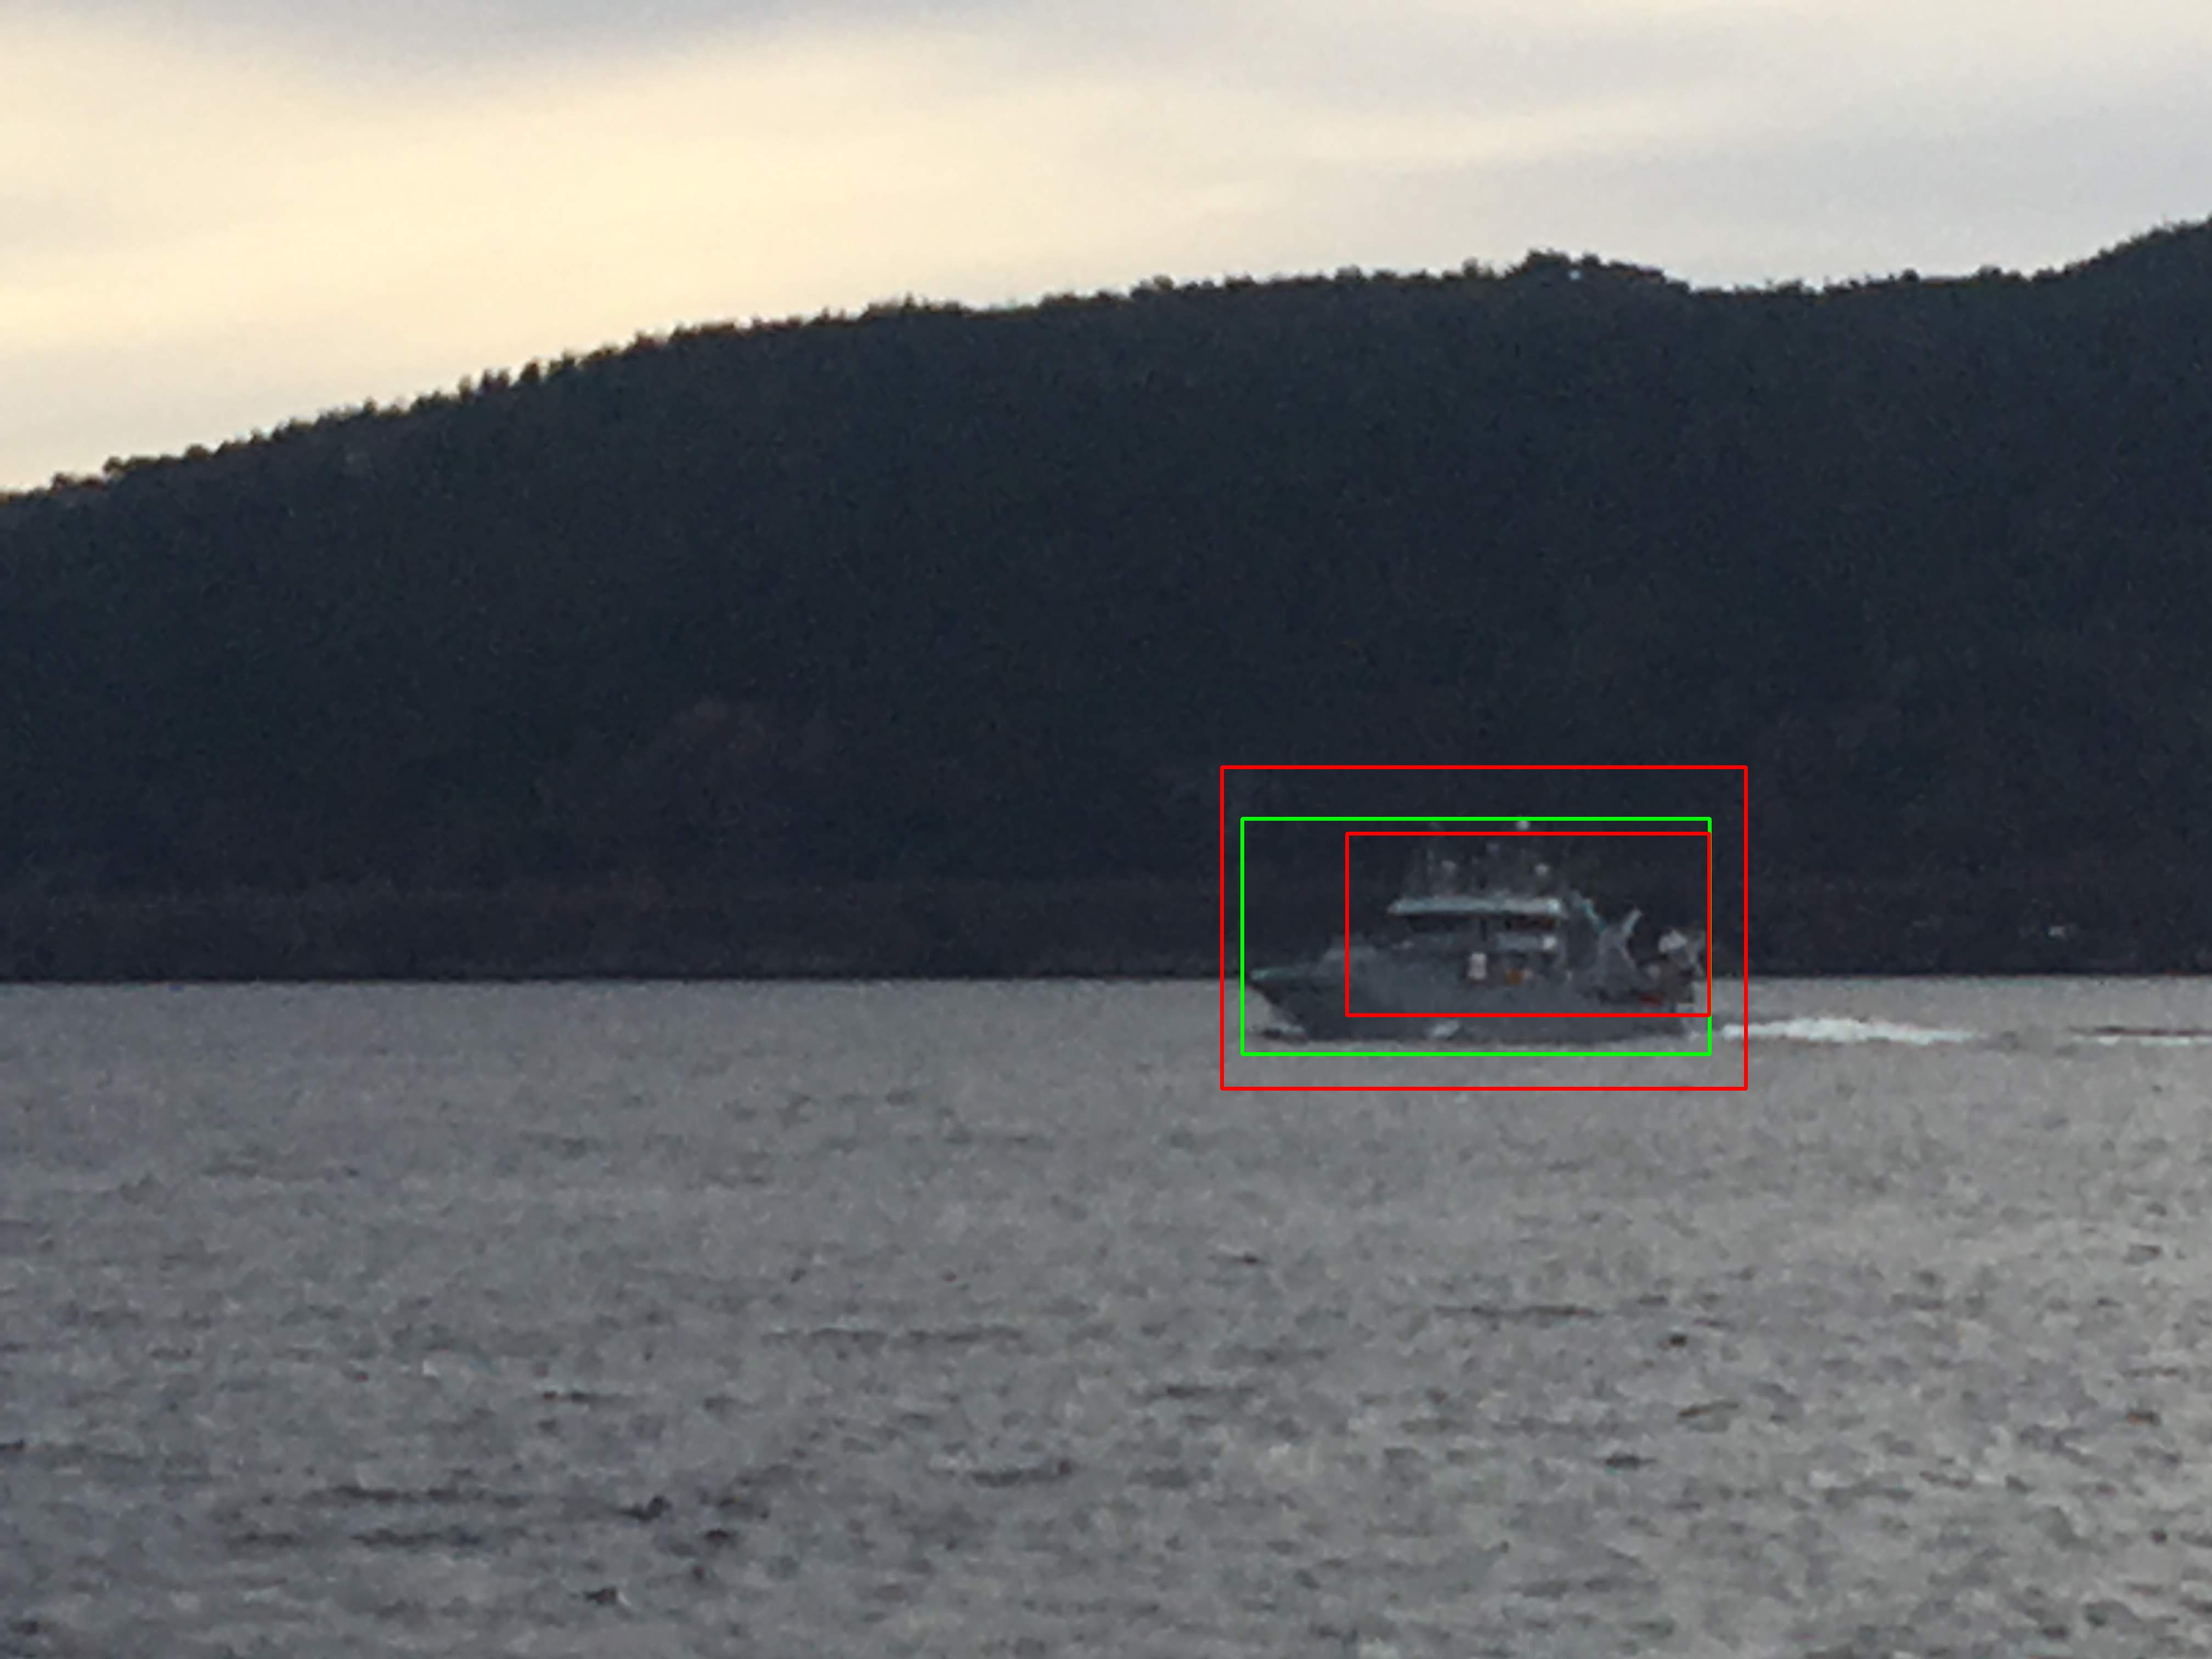
\includegraphics[width=0.8\linewidth]{results/case_tr_moor/yolo12/yolo1/2better/IMG_2269.jpg}
  \caption{Yolo1}
  \label{fig:yolo1_multibox}
\end{subfigure}%
\begin{subfigure}{.5\textwidth}
  \centering
  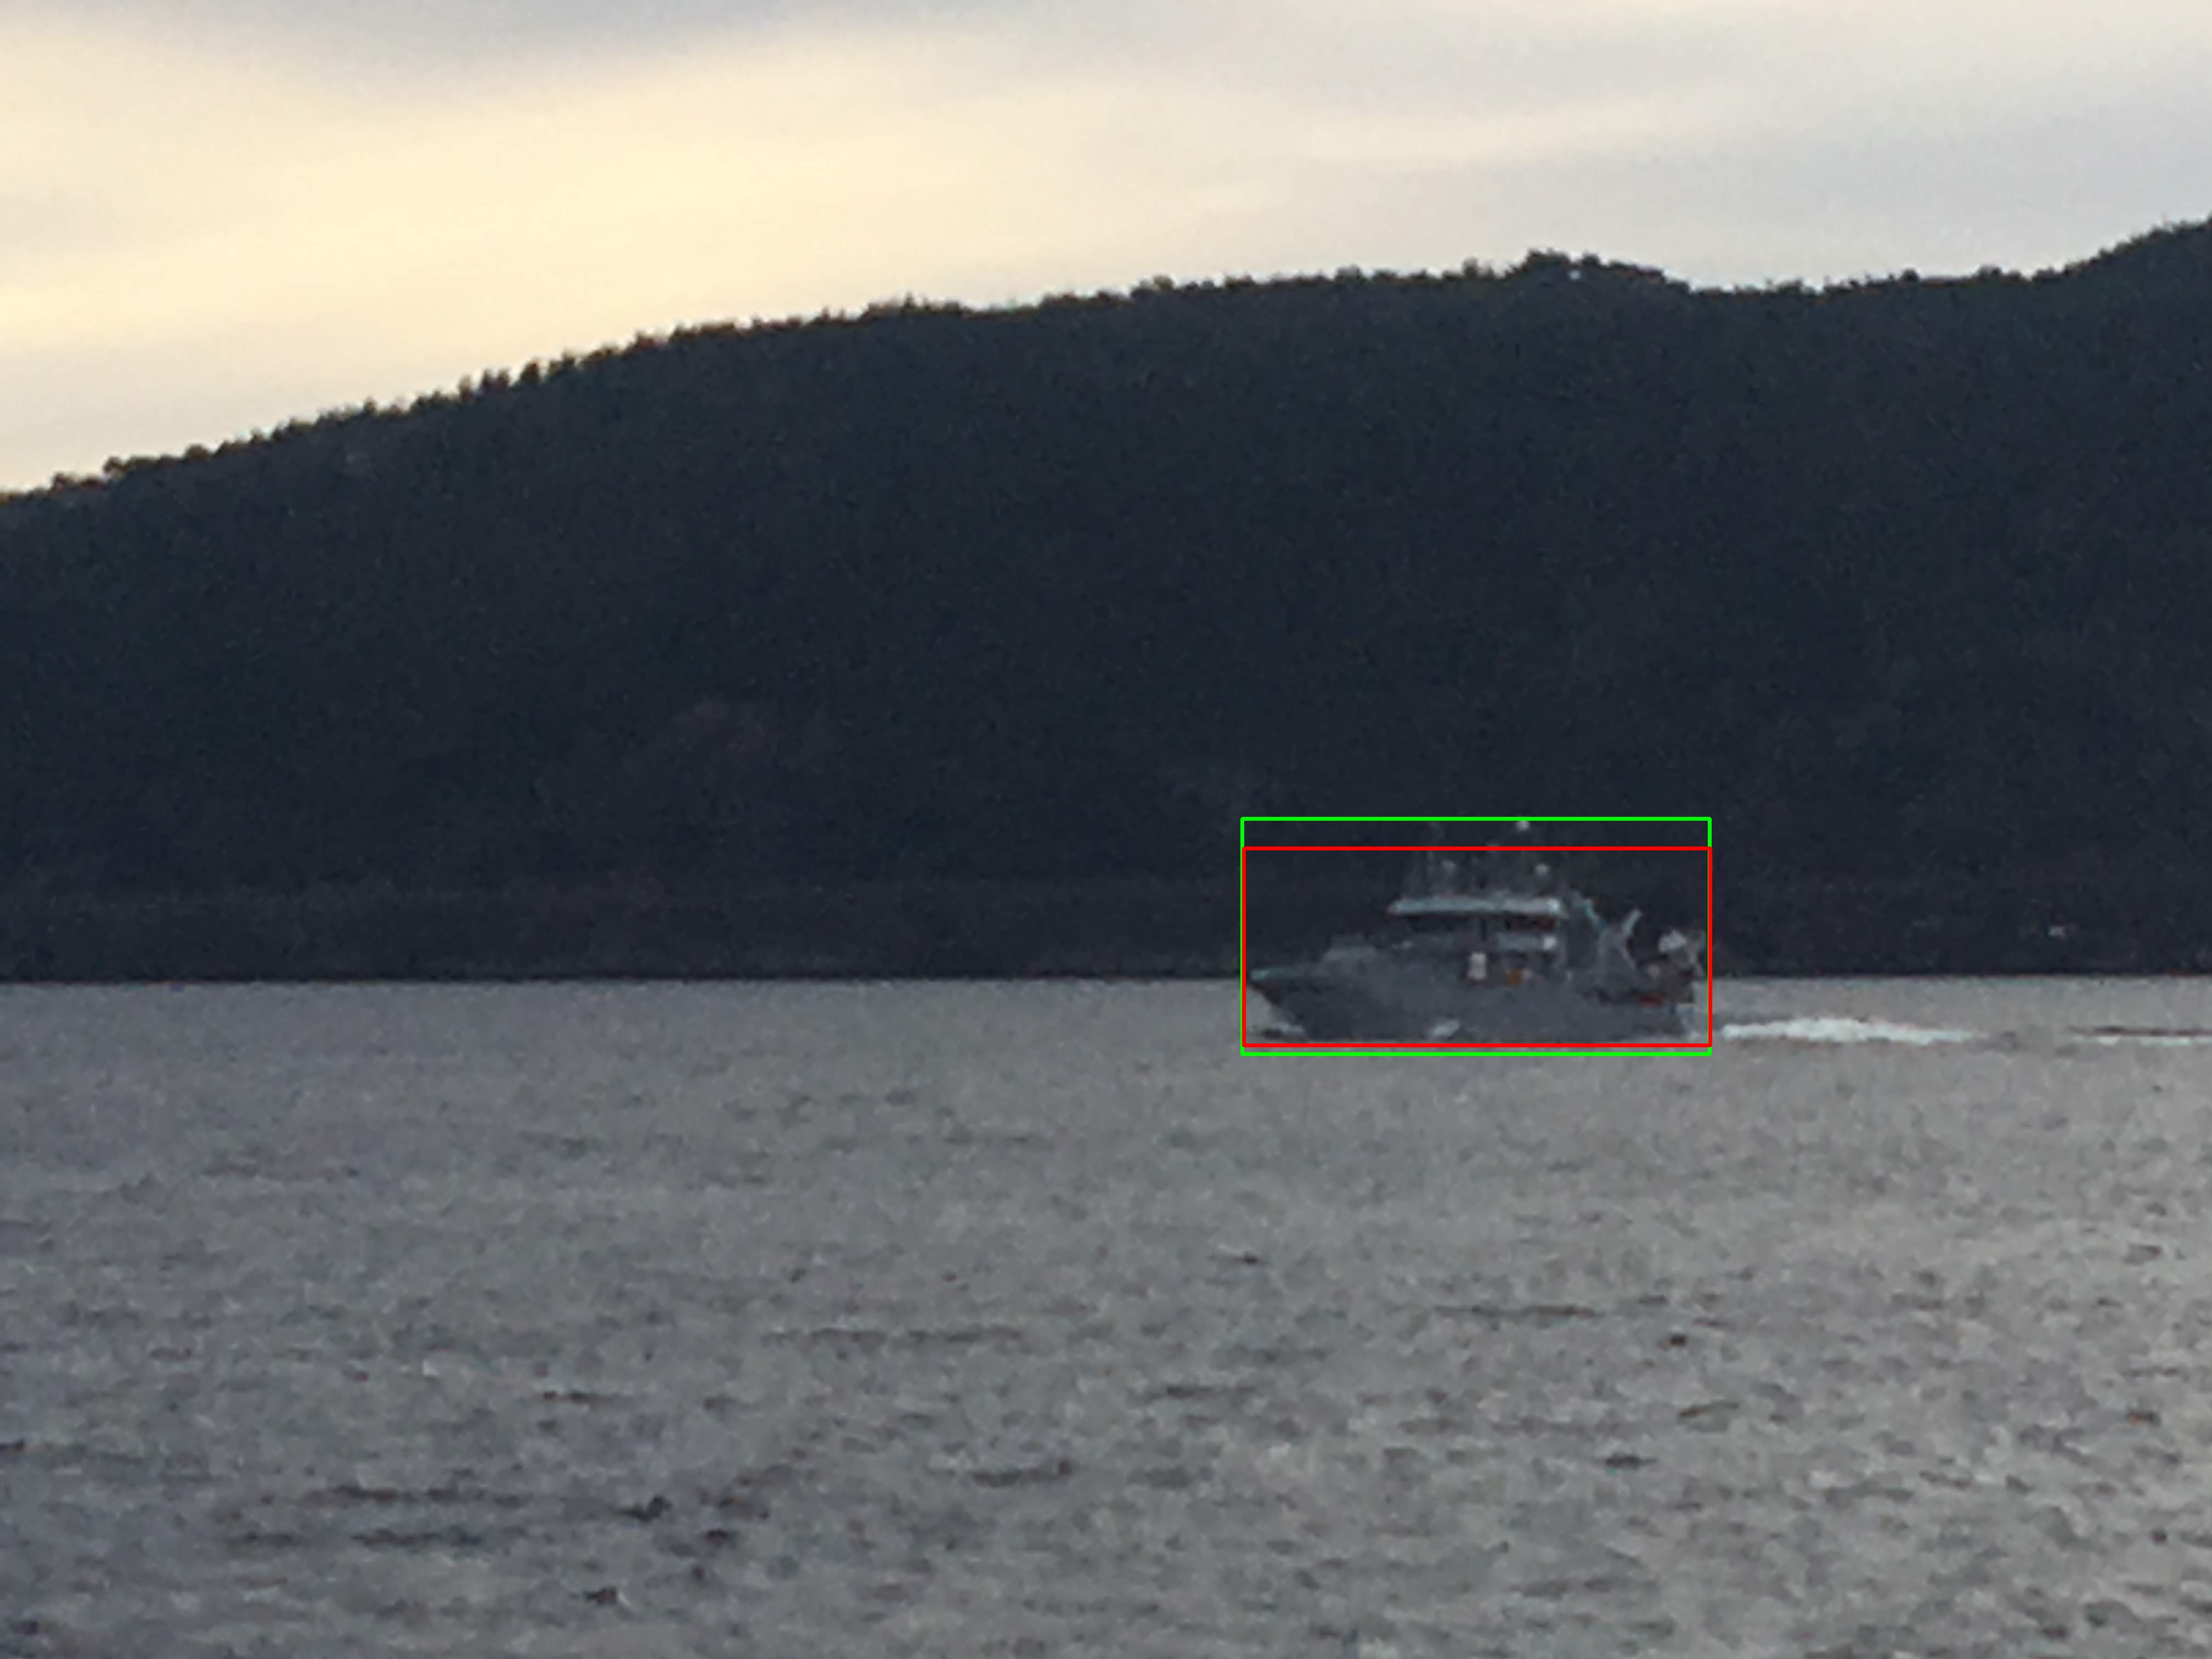
\includegraphics[width=.8\linewidth]{results/case_tr_moor/yolo12/yolo2/2better/IMG_2269.jpg}
  \caption{Yolo2}
  \label{fig:yolo2_multibox}
\end{subfigure}
\caption{Example of Yolo1 detecting same boat twice}
\label{fig:yolo12_multibox}
\end{figure}

\newpage

\section{Video streaks}
In \citep{Bohn2018} the issue of detection in data over time, such as e.g. video, is measured as \textit{streaks}. The goal is to make a detector that robustly detects boats in a video. This does not necessarily mean that the boat needs to be detected in every frame of a video since this can be solved e.g., by using a Markov chain as in \citep{Markov}. Still, the boat needs to be detected by some frequency, for the tracking algorithm to be able to track it. To implement a tracking algorithm is not a part of this project. However, an experiment on how well the detection algorithms work on video has been done. 

\vspace{3mm}

Three videos of boats in the Trondheim fjord has been captured, each approximately 20 seconds long. Yolo1 was run on each of them. The three videos are merged and available at \url{https://www.youtube.com/watch?v=kcirhao_PQc}. Frames from each of the videos are shown in figure \ref{fig:videos}.

\begin{figure}[h!]
\centering
\begin{subfigure}[b]{0.78\textwidth}
   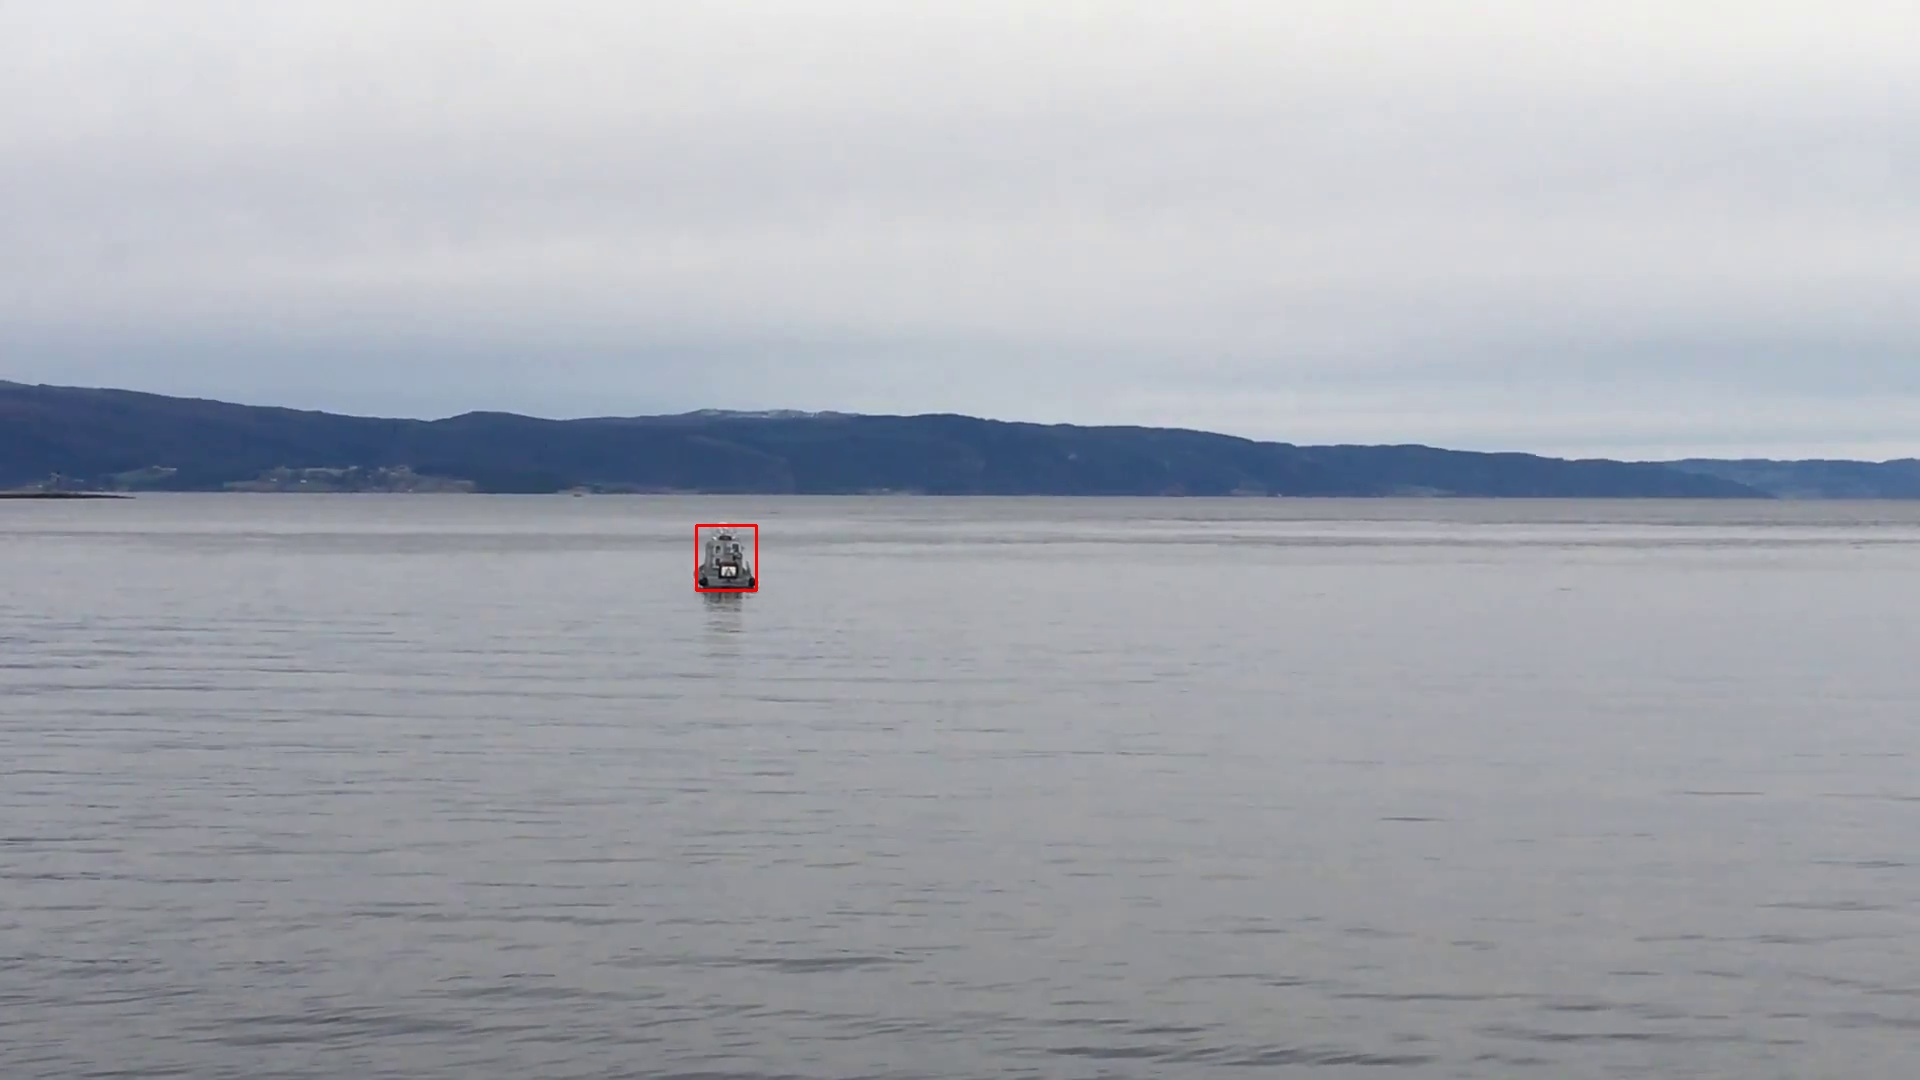
\includegraphics[width=1\linewidth]{results/video/video1/frame35.jpg}
   \caption{Video1}
   \label{fig:video1} 
\end{subfigure}

\begin{subfigure}[b]{0.78\textwidth}
   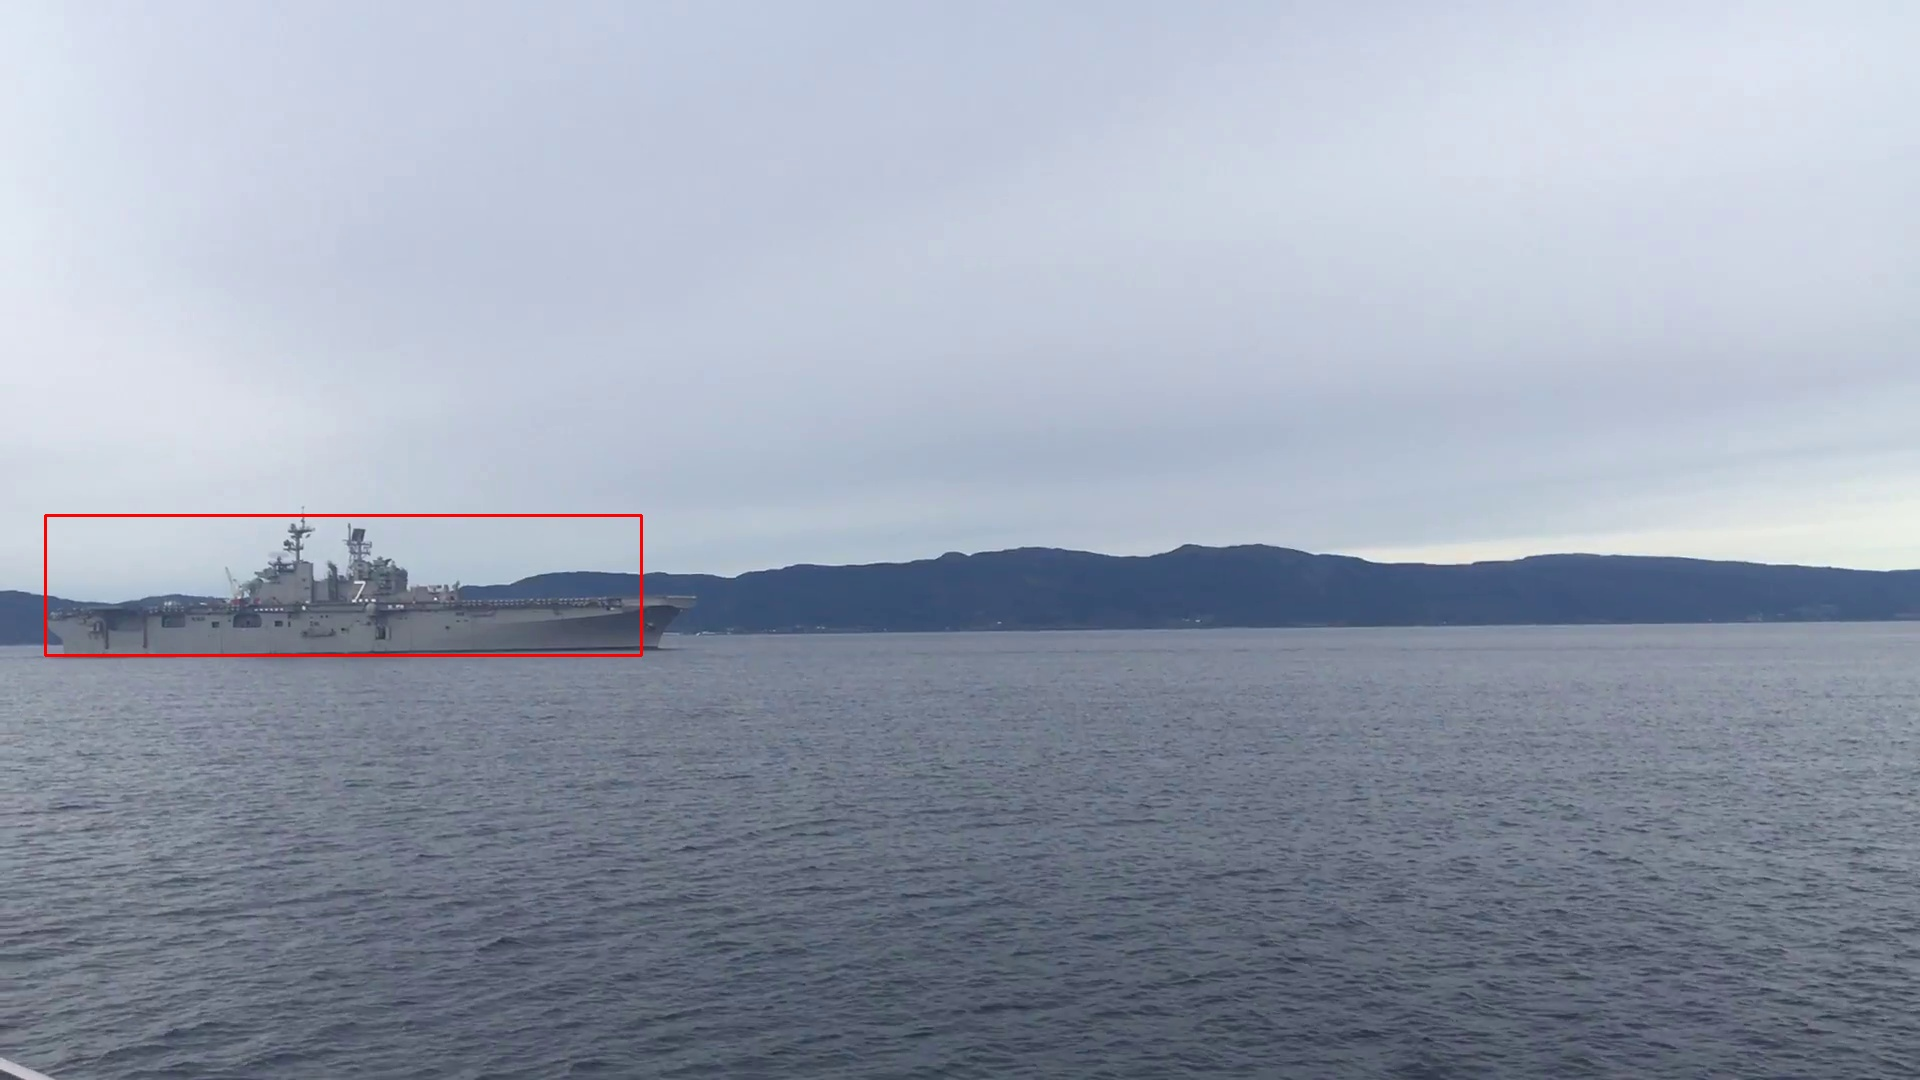
\includegraphics[width=1\linewidth]{results/video/video2/frame3.jpg}
   \caption{Video2}
   \label{fig:video2}
\end{subfigure}

\begin{subfigure}[b]{0.78\textwidth}
   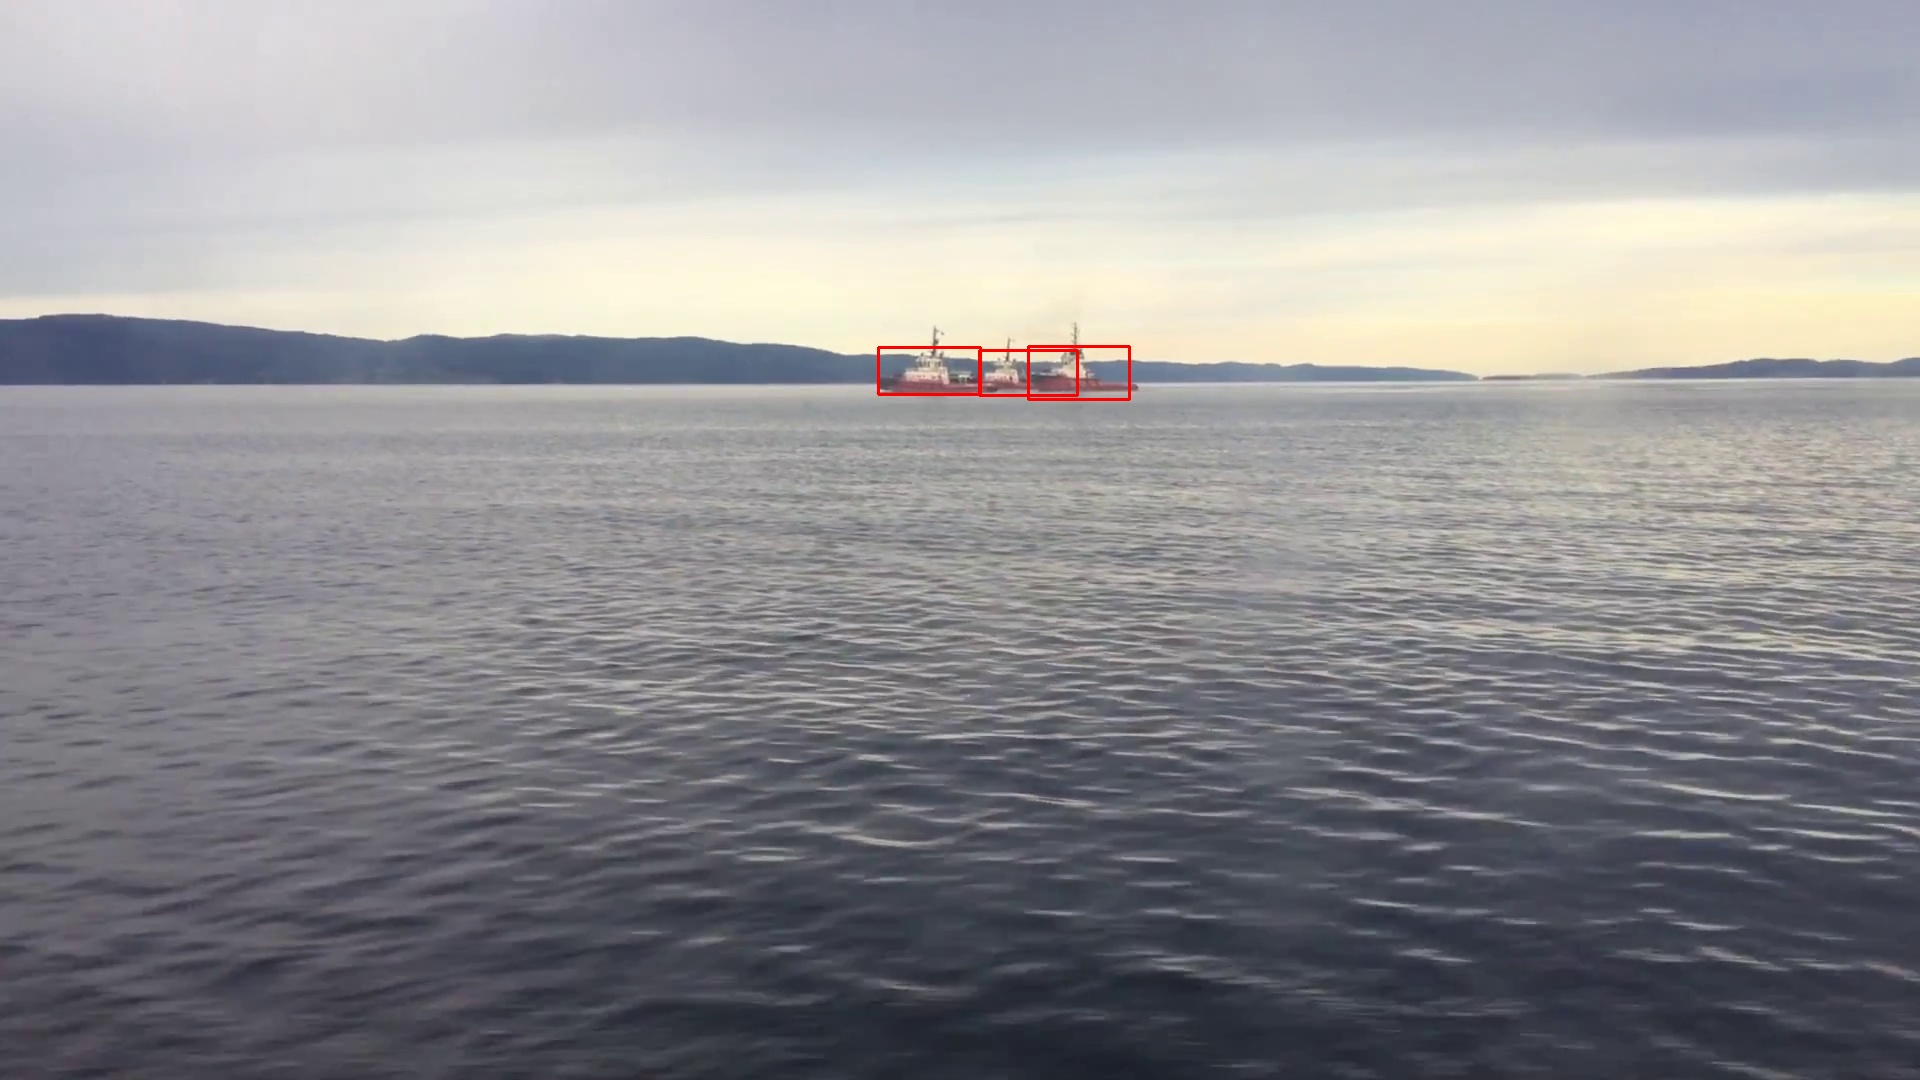
\includegraphics[width=1\linewidth]{results/video/video3/frame20.jpg}
   \caption{Video3}
   \label{fig:video3}
\end{subfigure}
\caption{Frames from video1, video2 and video3}
\label{fig:videos}
\end{figure}

\newpage

In video1 and video2 the boat is detected correctly in every frame. Thus streaks is not an issue in these videos. In both video1 and video2, there is only one boat present. In video3 there are three boats, where one of the boats passes behind another during the video. Yolo1 detects the boats in all frames where the boats are separated, as shown in figure \ref{fig:video3_sep}. When the third boat is behind the second, and beginning to emerge behind it, Yolo1 detects the two boats as one. This is shown in figure \ref{fig:video3_bigboat}. When the third boat is only slightly visible by human assessment, Yolo1 only detects two boats as shown in figure \ref{fig:video3_slightly}. 

\begin{figure}[h!]
\centering
\begin{subfigure}[b]{0.78\textwidth}
   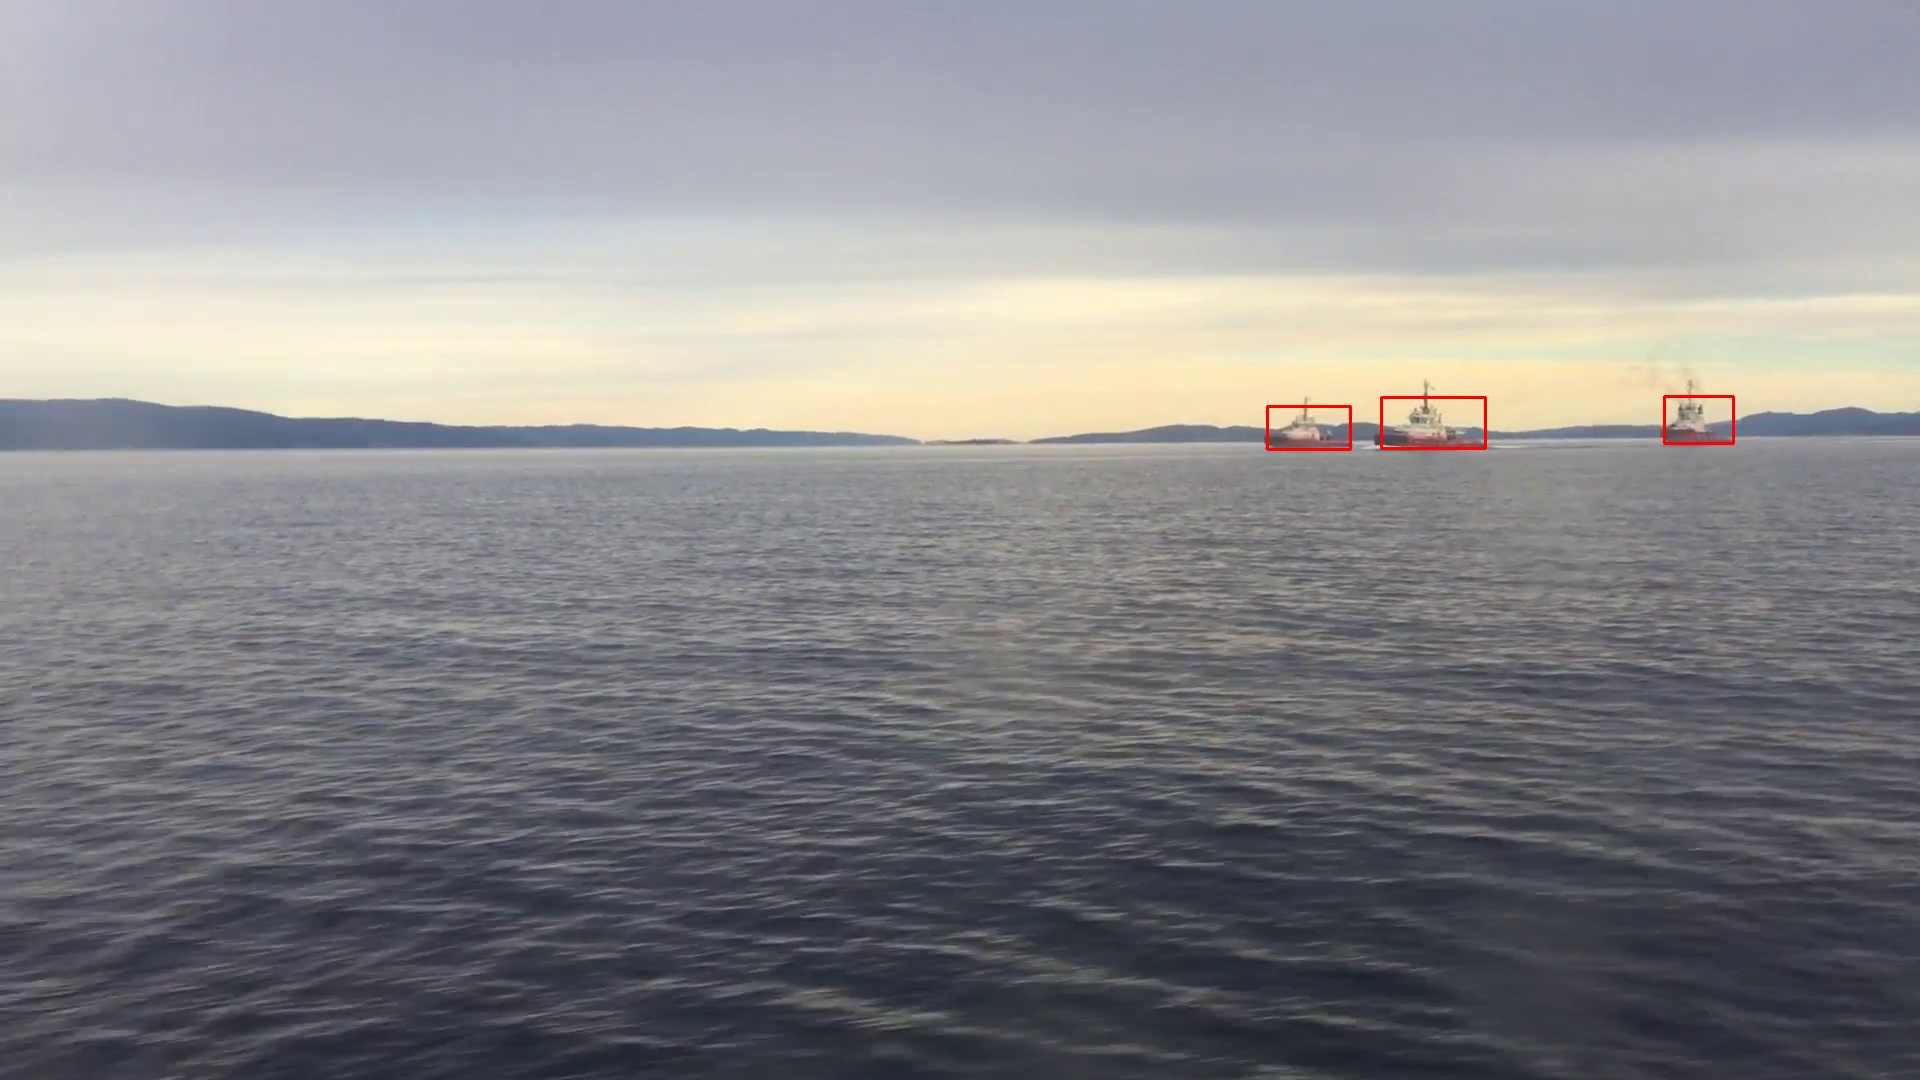
\includegraphics[width=1\linewidth]{results/video/video3/frame677.jpg}
   \caption{Three separated boats}
   \label{fig:video3_sep} 
\end{subfigure}

\begin{subfigure}[b]{0.78\textwidth}
   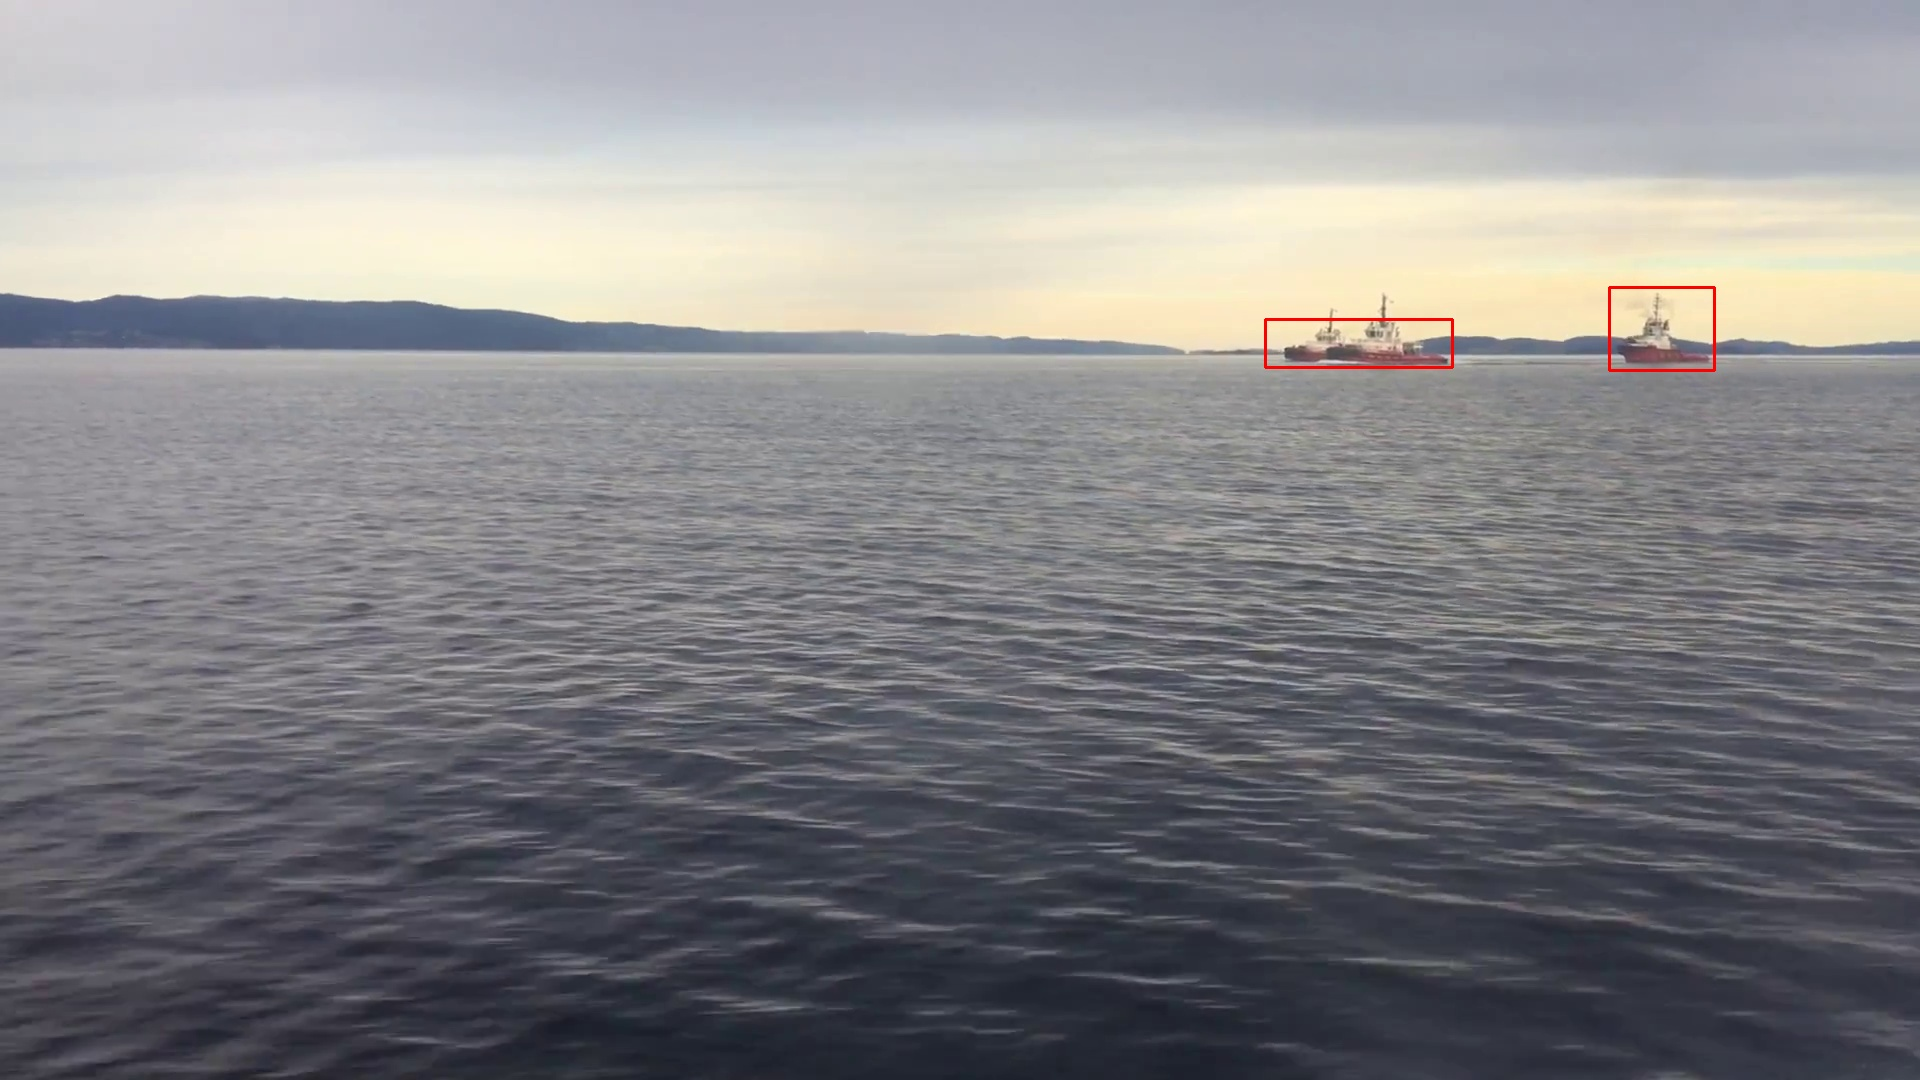
\includegraphics[width=1\linewidth]{results/video/video3/frame479.jpg}
   \caption{Part of third boat clearly visible}
   \label{fig:video3_bigboat}
\end{subfigure}

\begin{subfigure}[b]{0.78\textwidth}
   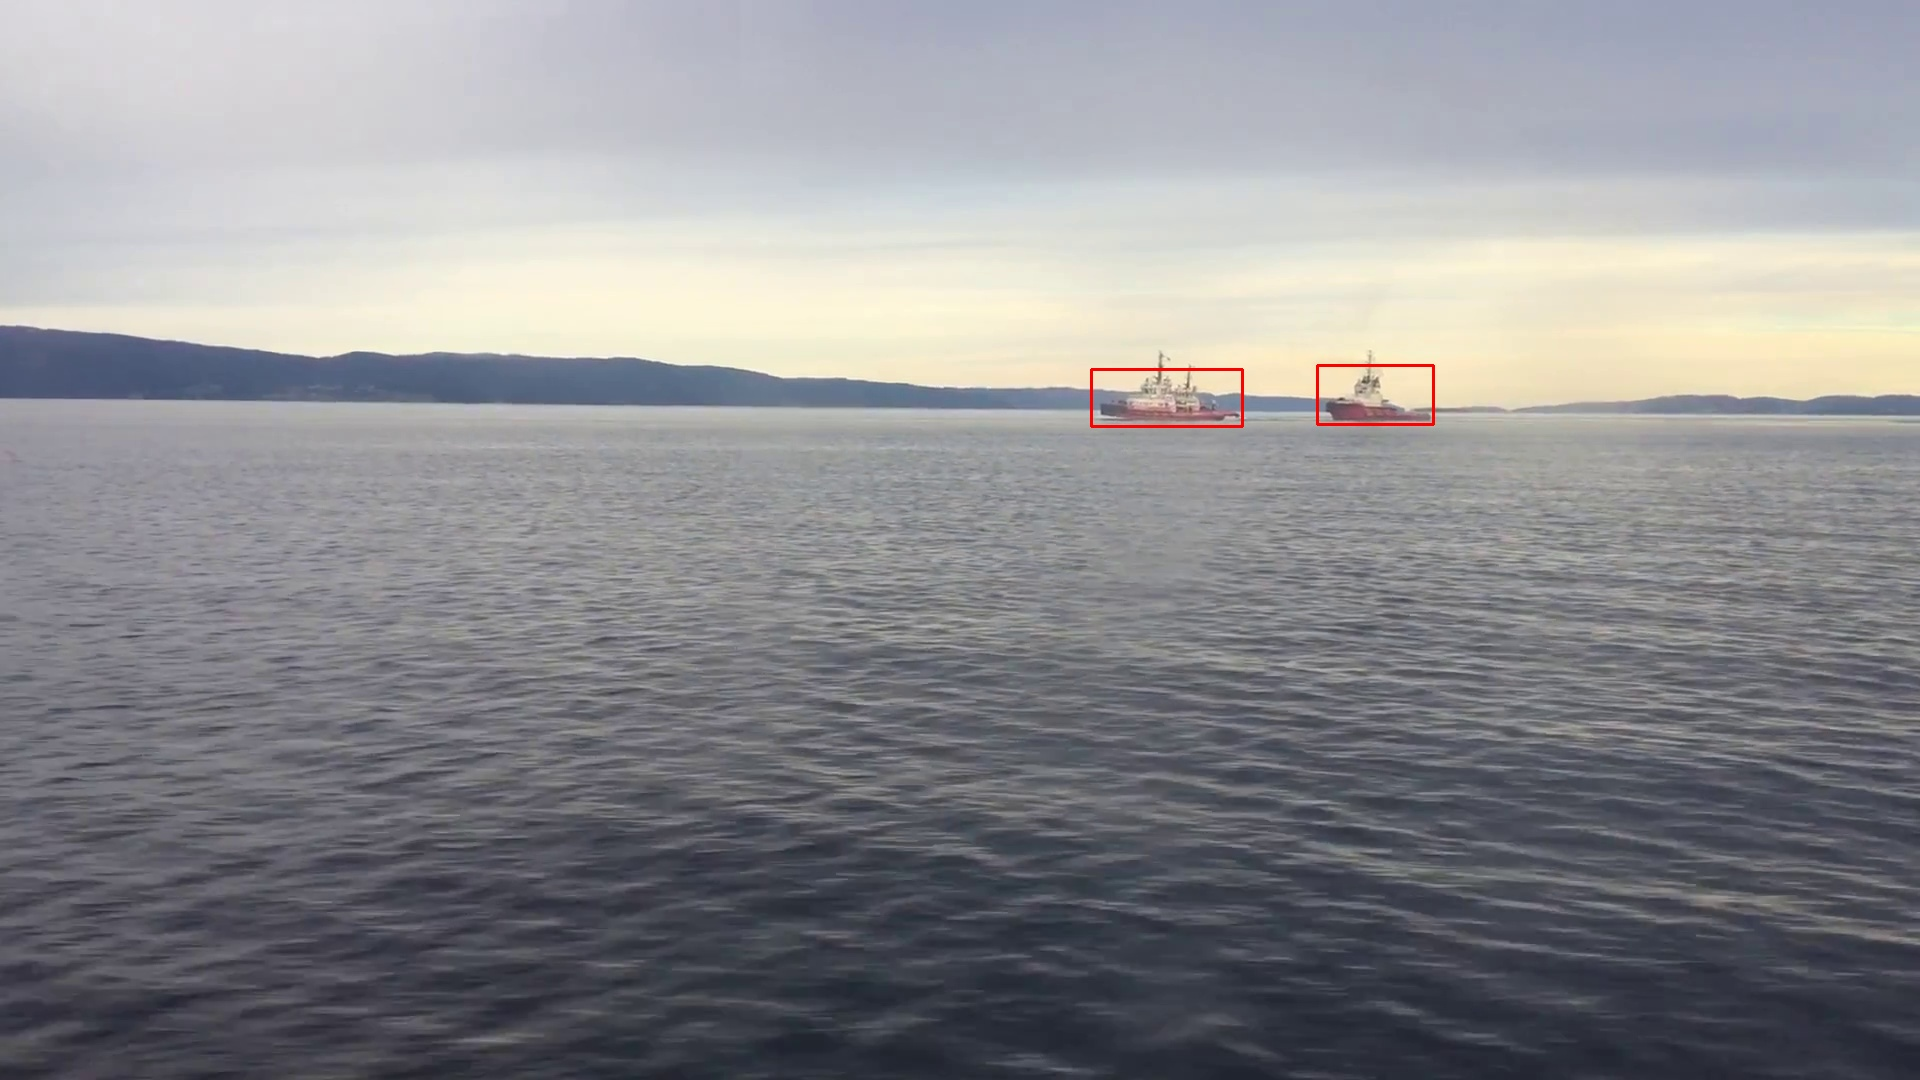
\includegraphics[width=1\linewidth]{results/video/video3/frame208.jpg}
   \caption{Third boat slightly visible}
   \label{fig:video3_slightly}
\end{subfigure}
\caption{Example frames from Video3}
\label{fig:video3}
\end{figure}

\newpage

In video3 all parts of boats are detected as boats, though two boats are classified as one big boat instead of two smaller ones when one is in the shadow of the other. This is a hard problem to solve for an object detector alone, and will be discussed further in chapter \ref{sec:boat_parts}. 


